\artpart{Operads in Categories}

\section{Background: $2$-monads and their Algebras}

\ngnoteil{insert something like: we assume basic familiarity with 2-categories, but still review $2$-monads stuff}
To investigate operads in $\cat$ we will make use of $2$-monads and their algebras, specifically the notion of pseudoalgebra for a $2$-monad. We assume familiarity with basic $2$-category theory, but cover the required definitions and theory related to $2$-monads here. For further reference, we refer the reader to \cite{BKP} and \cite{power-gen}.

\begin{Defi}[($2$-monad)]\label{Defi:2monad}
Let $\m{K}$ be a 2-category. A \emph{$2$-monad} on $\m{K}$ consists of
    \begin{itemize}
        \item a strict $2$-functor $T \colon \m{K} \rightarrow \m{K}$,
        \item a $2$-natural transformation $\mu \colon T^2 \Rightarrow T$,
        \item a $2$-natural transformation $\eta \colon \id_{\m{K}} \Rightarrow T$,
    \end{itemize}
satisfying the following axioms.
    \begin{itemize}
        \item The following diagram commutes.
        \[
            \xy
                (0,0)*+{T^3X}="00";
                (20,0)*+{T^2X}="10";
                (0,-15)*+{T^2X}="01";
                (20,-15)*+{TX}="11";
                {\ar^{T\mu_X} "00" ; "10"};
                {\ar^{\mu_x} "10" ; "11"};
                {\ar_{\mu_{TX}} "00" ;  "01"};
                {\ar_{\mu_X} "01" ; "11"};
            \endxy
        \]
        \item The following diagram commutes.
        \[
            \xy
                (0,0)*+{TX}="00";
                (20,0)*+{T^2X}="10";
                (40,0)*+{TX}="20";
                (20,-15)*+{TX}="11";
                %
                {\ar^{\eta_{TX}} "00" ; "10"};
                {\ar_{T\eta_X} "20" ; "10"};
                {\ar|{\mu_X} "10" ; "11"};
                {\ar_{\id_{TX}} "00" ; "11"};
                {\ar^{\id{TX}} "20" ; "11"};
            \endxy
        \]
\end{Defi}

\begin{Defi}[(Pseudoalgebra, $2$-monad version)]\label{Defi:pseudoalgebra}
Let $T \colon \m{K} \rightarrow \m{K}$ be a $2$-monad. A $T$-\textit{pseudoalgebra} consists of an object $X$, a $1$-cell $\alpha \colon TX \rightarrow X$ in $\m{K}$, and invertible $2$-cells of $\m{K}$
    \[
        \xy
            (0,0)*+{T^2X}="00";
            (20,0)*+{TX}="10";
            (0,-15)*+{TX}="01";
            (20,-15)*+{X}="11";
            {\ar^{T\alpha} "00" ; "10"};
            {\ar^{\alpha} "10" ; "11"};
            {\ar_{\mu_X} "00" ;  "01"};
            {\ar_{\alpha} "01" ; "11"};
            {\ar@{=>}^{\Phi} (10,-5.5) ; (10,-9.5)};
            (40,0)*+{X}="20";
            (52.5,-15)*+{TX}="31";
            (72.5,-15)*+{X}="41";
            {\ar_{\eta_X} "20" ; "31"};
            {\ar_{\alpha} "31" ; "41"};
            {\ar@/^1.5pc/^{1_X} "20" ; "41"};
            {\ar@{=>}^{\Phi_{\eta}} (54.5,-5.5) ; (54.5,-9.5)};
        \endxy
    \]

satisfying the following axioms.
    \begin{itemize}
        \item The following equality of pasting diagrams holds.
    \[
        \xy
            (5,0)*+{T^3X}="t3xl";
            (29,0)*+{T^2X}="t2xl1";
            (5,-17.5)*+{T^2X}="t2xl2";
            (24,-35)*+{TX}="txl1";
            (48,-17.5)*+{TX}="txl2";
            (48,-35)*+{X}="xl";
            (24,-17.5)*+{T^2X}="t2xl3";
            {\ar^{T^2\alpha} "t3xl" ; "t2xl1"};
            {\ar^{T\alpha} "t2xl1" ; "txl2"};
            {\ar^{\alpha} "txl2" ; "xl"};
            {\ar_{\mu_{TX}} "t3xl" ; "t2xl2"};
            {\ar_{\mu_X} "t2xl2" ; "txl1"};
            {\ar_{\alpha} "txl1" ; "xl"};
            {\ar_{T\mu_X} "t3xl" ; "t2xl3"};
            {\ar^{T\alpha} "t2xl3" ; "txl2"};
            {\ar_{\mu_X} "t2xl3" ; "txl1"};
            {\ar@{=>}_{T\Phi} (26,-6) ; (26,-10)};
            {\ar@{=>}^{\Phi} (36,-24) ; (36,-28)};
            (64,0)*+{T^3X}="t3xr";
            (88,0)*+{T^2X}="t2xr1";
            (64,-17.5)*+{T^2X}="t2xr2";
            (83,-35)*+{TX}="txr1";
            (107,-17.5)*+{TX}="txr2";
            (107,-35)*+{X}="xr";
            (88,-17.5)*+{TX}="txr3";
            {\ar^{T^2\alpha} "t3xr" ; "t2xr1"};
            {\ar^{T\alpha} "t2xr1" ; "txr2"};
            {\ar^{\alpha} "txr2" ; "xr"};
            {\ar_{\mu_{TX}} "t3xr" ; "t2xr2"};
            {\ar_{\mu_X} "t2xr2" ; "txr1"};
            {\ar_{\alpha} "txr1" ; "xr"};
            {\ar_{T\alpha} "t2xr2" ; "txr3"};
            {\ar_{\alpha} "txr3" ; "xr"};
            {\ar_{\mu_X} "t2xr1" ; "txr3"};
            {\ar@{=>}_{\Phi} (98,-15) ; (98,-19)};
            {\ar@{=>}^{\Phi} (85,-24) ; (85,-28)};
            {\ar@{=} (54,-20) ; (56,-20)};
        \endxy
    \]

    \item The following pasting diagram is an identity.
    \[
        \xy
            (0,0)*+{TX}="txl1";
            (15,-15)*+{T^2X}="t2x";
            (15,-30)*+{TX}="txl2";
            (35,-15)*+{TX}="txl3";
            (35,-30)*+{X}="xl";
            {\ar@/^1.7pc/^{1_{TX}} "txl1" ; "txl3"};
            {\ar@/_1.7pc/_{1_{TX}} "txl1" ; "txl2"};
            {\ar_{T\eta_X} "txl1" ; "t2x"};
            {\ar^{T\alpha} "t2x" ; "txl3"};
            {\ar_{\mu_X} "t2x" ; "txl2"};
            {\ar_{\alpha} "txl2" ; "xl"};
            {\ar^{\alpha} "txl3" ; "xl"};
            {\ar@{=>}^{T\Phi_\eta} (17,-5.5) ; (17,-9.5)};
            {\ar@{=>}^{\Phi} (25,-20.5) ; (25,-24.5)};
        \endxy
    \]

    \end{itemize}
\end{Defi}

Power's definition of a pseudoalgebra includes a third axiom relating to the unit of the $2$-monad \cite[Definition 2.4, Axiom 2.1]{power-gen}. However, following an argument of Marmolejo \cite[Lemma 9.1]{marm-doct} this extra axiom is redundant and is omitted here.

\begin{Defi}[(Strict algebra, $2$-monad version)]\label{Defi:strictalgebra}
Let $T \colon \m{K} \rightarrow \m{K}$ be a $2$-monad. A \textit{strict $T$-algebra} is a pseudoalgebra in which all of the isomorphisms $\Phi$ are identities.
\end{Defi}

\begin{Defi}[(Pseudomorphism, $2$-monad version)]\label{Defi:pseudomorphism}
Let $T$ be a $2$-monad and let $(X,\alpha,\Phi,\Phi_\eta)$, $(Y,\beta,\Psi,\Psi_\eta)$ be $T$-pseudoalgebras. A \textit{pseudomorphism} $(f, \bar{f})$ between these pseudoalgebras consists of a $1$-cell $f \colon X \rightarrow Y$ along with an invertible $2$-cell
    \[
        \xy
            (0,0)*+{TX}="00";
            (20,0)*+{TY}="10";
            (0,-15)*+{X}="01";
            (20,-15)*+{Y}="11";
            {\ar^{Tf} "00" ; "10"};
            {\ar^{\beta} "10" ; "11"};
            {\ar_{\alpha} "00" ; "01"};
            {\ar_{f} "01" ; "11"};
            {\ar@{=>}^{\bar{f}} (10,-5.5) ; (10,-9.5)};
        \endxy
    \]

satisfying the following axioms.
    \begin{itemize}
        \item The following equality of pasting diagrams holds.
                \[
        \xy
            (5,0)*+{T^2X}="t3xl";
            (29,0)*+{T^2Y}="t2xl1";
            (5,-17.5)*+{TX}="t2xl2";
            (24,-35)*+{TX}="txl1";
            (48,-17.5)*+{TY}="txl2";
            (48,-35)*+{Y}="xl";
            (24,-17.5)*+{TX}="t2xl3";
            {\ar^{T^2f} "t3xl" ; "t2xl1"};
            {\ar^{T\beta} "t2xl1" ; "txl2"};
            {\ar^{\beta} "txl2" ; "xl"};
            {\ar_{\mu_X} "t3xl" ; "t2xl2"};
            {\ar_{\alpha} "t2xl2" ; "txl1"};
            {\ar_{f} "txl1" ; "xl"};
            {\ar^{T\alpha} "t3xl" ; "t2xl3"};
            {\ar^{Tf} "t2xl3" ; "txl2"};
            {\ar_{\alpha} "t2xl3" ; "txl1"};
            {\ar@{=>}^{T\bar{f}} (24,-6) ; (24,-10)};
            {\ar@{=>}^{\bar{f}} (36,-24) ; (36,-28)};
            {\ar@{=>}^{\Phi} (13.5,-15.5) ; (13.5,-19.5)};
            (64,0)*+{T^2X}="t3xr";
            (88,0)*+{T^2Y}="t2xr1";
            (64,-17.5)*+{TX}="t2xr2";
            (83,-35)*+{TX}="txr1";
            (107,-17.5)*+{TY}="txr2";
            (107,-35)*+{Y}="xr";
            (88,-17.5)*+{TX}="txr3";
            {\ar^{T^2f} "t3xr" ; "t2xr1"};
            {\ar^{T\beta} "t2xr1" ; "txr2"};
            {\ar^{\beta} "txr2" ; "xr"};
            {\ar_{\mu_{X}} "t3xr" ; "t2xr2"};
            {\ar_{\alpha} "t2xr2" ; "txr1"};
            {\ar_{f} "txr1" ; "xr"};
            {\ar_{Tf} "t2xr2" ; "txr3"};
            {\ar_{\beta} "txr3" ; "xr"};
            {\ar_{\mu_Y} "t2xr1" ; "txr3"};
            {\ar@{=>}_{\Psi} (98,-15) ; (98,-19)};
            {\ar@{=>}^{\bar{f}} (85,-24) ; (85,-28)};
            {\ar@{=} (54,-20) ; (56,-20)};
        \endxy
    \]
    %redraw with tikzpicture
    \item The following equality of pasting diagrams holds.
            \[
                        \xy
            (0,0)*+{X}="00";
            (20,0)*+{Y}="10";
            (0,-20)*+{TX}="01";
            (20,-20)*+{TY}="11";
            (10,-35)*+{X}="02";
            (30,-35)*+{Y}="12";
            {\ar^{f} "00" ; "10"};
            {\ar@/^1.5pc/^{1_Y} "10" ; "12"};
            {\ar_{\eta_X} "00" ; "01"};
            {\ar_{\eta_Y} "10" ; "11"};
            {\ar_{Tf} "01" ; "11"};
            {\ar_{\alpha} "01" ; "02"};
            {\ar_{f} "02" ; "12"};
            {\ar^{\beta} "11" ; "12"};
            {\ar@{=>}^{\bar{f}} (15,-25.5) ; (15,-29.5)};
            {\ar@{=>}^{\Psi_{\eta}} (25,-17) ; (25,-21)};
            (50,0)*+{X}="30";
            (70,0)*+{Y}="40";
            (50,-20)*+{TX}="31";
            (60,-35)*+{X}="32";
            (80,-35)*+{Y}="42";
            {\ar^{f} "30" ; "40"};
            {\ar_{\eta_X} "30" ; "31"};
            {\ar_{\alpha} "31" ; "32"};
            {\ar_{f} "32" ; "42"};
            {\ar@/^1.5pc/^{1_X} "30" ; "32"};
            {\ar@/^1.5pc/^{1_Y} "40" ; "42"};
            {\ar@{=>}^{\Phi_{\eta}} (55,-17) ; (55,-21)};
        \endxy
        \]
        %redraw with tikzpicture

\end{itemize}
\end{Defi}

\begin{Defi}[(Strict morphism, $2$-monad verison)]\label{Defi:strictmorphism}
Let $T$ be a $2$-monad and let $(X,\alpha,\Phi,\Phi_\eta)$ and $(Y,\beta,\Psi,\Psi_\eta)$ be $T$-pseudoalgebras. A \textit{strict morphism} $(f, \bar{f})$ consists of a pseudomorphism in which $\bar{f}$ is an identity.
\end{Defi}

\begin{rem}
The strict algebras and strict morphisms are exactly the same as algebras and morphisms for the underlying monad on the underlying category of $\m{K}$.
\end{rem}

\begin{Defi}[($T$-transformation, $2$-monad version)]\label{Defi:Ttrans}
Let $(f, \overline{f}), (g, \overline{g}) \colon X \rightarrow Y$ be pseudomorphisms of $T$-algebras. A \textit{$T$-transformation} consists of a $2$-cell $\gamma \colon f \Rightarrow g$ such that the following equality of pasting diagrams holds.
    \[
        \xy
            (0,0)*+{TX}="00";
            (30,0)*+{TY}="10";
            (0,-20)*+{X}="01";
            (30,-20)*+{Y}="11";
            {\ar@/^1.5pc/^{Tf} "00" ; "10"};
            {\ar_{Tg} "00" ; "10"};
            {\ar^{\beta} "10" ; "11"};
            {\ar_{\alpha} "00" ; "01"};
            {\ar_{g} "01" ; "11"};
            {\ar@{=>}^{T \gamma} (13.5,5.5) ; (13.5,1.5)};
            {\ar@{=>}^{\overline{g}} (13.5,-8) ; (13.5,-12)};
            (60,0)*+{TX}="x00";
            (90,0)*+{TY}="x10";
            (60,-20)*+{X}="x01";
            (90,-20)*+{Y}="x11";
            {\ar^{Tf} "x00" ; "x10"};
            {\ar^{\beta} "x10" ; "x11"};
            {\ar_{\alpha} "x00" ; "x01"};
            {\ar^{f} "x01" ; "x11"};
            {\ar@/_1.5pc/_{g} "x01" ; "x11"};
            {\ar@{=>}^{\gamma} (75,-21.5) ; (75,-25.5)};
            {\ar@{=>}^{\overline{f}} (75,-8) ; (75,-12)};
            {\ar@{=} (42.75,-10) ; (46.75,-10)};
        \endxy
    \]
    %redraw with tikzpicture

\end{Defi}

There are many different possible choices of 2-categories in which the objects are some kind of algebra over a $2$-monad $T$.
Here are the two that will be the most important for us.

\begin{Defi}[(2-categories of algebras, $2$-monad version)]\label{Defi:2cat-of-algs}
Let $T$ be a $2$-monad.
\begin{itemize}
\item The $2$-category $T\mbox{-}\mb{Alg}_{s}$ consists of strict $T$-algebras, strict morphisms, and $T$-transformations.
\item The $2$-category $\mb{Ps}\mbox{-}T\mbox{-}\mb{Alg}$ consists of $T$-pseudoalgebras, pseudomorphisms, and $T$-transformations.
\end{itemize}
\end{Defi}

\section{\texorpdfstring{$\Lambda$}{L}-Operads in Cat as $2$-monads}

This section begins our study of algebras over a $\Lambda$-operad $P$ in $\mb{Cat}$.
This theory blends together standard results in both $2$-monad theory\ngnote{lack codescent, bkp} and operad theory\ngnote{may geometry of iterated loops}.

\begin{conv}[(Sets and discrete categories)]\label{conv:set-disc}
Throughout the rest of this text, $\Lambda$ will be an action in the category of sets.
By abuse of notation, any set $S$ will be identified with the discrete, small category $dS$ with object set $S$.
In this way, we also view any action operad $\Lambda$ as an operad in $\mb{Cat}$, and we view any group $G$ as a discrete, strict monoidal category.
\end{conv}

\begin{conv}[(Group actions on categories)]\label{conv:group-act-cat}
A group action on a category is meant in the strict sense, not in the up-to-isomorphism sense.
Thus if $G$ acts on $C$, the equations
\begin{align*}
g \cdot (h \cdot x) & = (gh) \cdot x,\\
1 \cdot x & = x
\end{align*}
hold for all $x$, where $x$ is allowed to be either an object or morphism of $C$.
\end{conv}


\begin{rem}[($\Lambda$-operads in $\mb{Cat}$)]\label{rem:lop-in-cat}
Here we explicitly describe the structure of a $\Lambda$-operad $P$ in $\mb{Cat}$, following \cref{rem:sec8-in-V}.
\ngnoteil{details plz}
\end{rem}

\begin{Defi}[(Pseudoalgebra, $\Lambda$-operad version)]\label{def:ps-alg-lop}
Let $P$ be a $\Lambda$-operad. A \textit{pseudoalgebra} for $P$ consists of: 
    \begin{itemize}
        \item a category $X$,
        \item a family of functors
            \[
                \left(\alpha_n \colon \coeq{P}{X}{\Lambda}{n} \rightarrow X \right)_{n \in \mathbb{N}},
            \]
        \item for each $n, k_1, \ldots, k_n \in \mathbb{N}$, a natural isomorphism $\phi_{k_1, \ldots, k_n}$ (corresponding, via Conventions \ref{conv_coeq}) to a natural isomorphism
            \[
                \xy
                    (0,0)*+{\scriptstyle P_n \times \prod_{i=1}^n \left(P_{k_i} \times X^{k_i}\right)}="00";
                    (0,-10)*+{\scriptstyle P_n \times \prod_{i=1}^n P_{k_i} \times X^{\Sigma k_i}}="01";
                    (0,-20)*+{\scriptstyle P_{\Sigma k_i} \times X^{\Sigma k_i}}="02";
                    (60,-20)*+{\scriptstyle X}="12";
                    (60,0)*+{\scriptstyle P_n \times X^n}="11";
                    {\ar_{} "00" ; "01"};
                    {\ar^{1 \times \prod \tilde{\alpha}_{k_i}} "00" ; "11"};
                    {\ar^{\tilde{\alpha}_n} "11" ; "12"};
                    {\ar_{\mu^P \times 1} "01" ; "02"};
                    {\ar_>>>>>>>>>>>>>>>>>>>{\tilde{\alpha}_{\Sigma k_i}} "02" ; "12"};
                    {\ar@{=>}^{\tilde{\phi}_{k_1, \ldots, k_n}} (30,-8) ; (30,-12)};
                \endxy
            \]

               \item and a natural isomorphism $\phi_{\eta}$ corresponding to a natural isomorphism
            \[
                \xy
                    (0,0)*+{X}="00";
                    (0,-15)*+{1 \times X}="x10";
                    (0,-30)*+{P(1) \times X}="10";
                    (30,-30)*+{X}="11";
                    {\ar_{\eta^P \times 1} "x10" ; "10"};
                    {\ar_{\tilde{\alpha}_1} "10" ; "11"};
                    {\ar^{1} "00" ; "11"};
                    {\ar_{\cong} "00" ; "x10"};
                    {\ar@{=>}^{\tilde{\phi}_\eta} (10,-18) ; (10,-22)};
                \endxy
            \]

    \end{itemize}
satisfying the following axioms.
    \begin{itemize}
        \item For all $n, k_i, m_{ij} \in \mathbb{N}$, the following equality of pasting diagrams holds.
            \[
                \xy
                    (0,0)*+{\scriptstyle P_n \times \prod_i\left(P_{k_i} \times \prod_j \left(P_{m_{ij}} \times X^{m_{ij}}\right)\right)}="00";
                    (60,0)*+{\scriptstyle P_n \times \prod_i \left(P_{k_i} \times X^{k_i}\right)}="10";
                    (0,-30)*+{\scriptstyle P_{\Sigma k_i} \times \prod_i\prod_j\left(P_{m_{ij}} \times X^{m_{ij}}\right)}="02";
                    (30,-50)*+{\scriptstyle P_{\Sigma\Sigma m_{ij}} \times X^{\Sigma \Sigma m_{ij}}}="04";
                    (80,-20)*+{\scriptstyle P_n \times X^n}="12";
                    (80,-50)*+{\scriptstyle X}="14";
                    {\ar^>>>>>>>>>>>>>>{1 \times \prod\left(1 \times \prod \tilde{\alpha}_{m_ij}\right)} "00" ; "10"};
                    {\ar^{1 \times \prod \tilde{\alpha}_{k_i}} "10" ; "12"};
                    {\ar^{\tilde{\alpha}_n} "12" ; "14"};
                    {\ar_{\mu^P \times 1} "00" ; "02"};
                    {\ar_{\mu^P \times 1} "02" ; "04"};
                    {\ar_{\tilde{\alpha}_{\Sigma\Sigma m_{ij}}} "04" ; "14"};
                    (30,-20)*+{\scriptstyle P_n \times \prod_i\left(P_{\Sigma m_{ij}} \times X^{\Sigma m_{ij}}\right)}="22";
                    {\ar^{\mu^P \times 1} "00" ; "22"};
                    {\ar^{1 \times \prod \tilde{\alpha}_{\Sigma m_{ij}}} "22" ; "12"};
                    {\ar^{\mu^P \times 1} "22" ; "04"};
                    (0,-70)*+{\scriptstyle P_n \times \prod_i\left(P_{k_i} \times \prod_j \left(P_{m_{ij}} \times X^{m_{ij}}\right)\right)}="b00";
                    (50,-70)*+{\scriptstyle P_n \times \prod_i \left(P_{k_i} \times X^{k_i}\right)}="b10";
                    (0,-100)*+{\scriptstyle P_{\Sigma k_i} \times \prod_i\prod_j\left(P_{m_{ij}} \times X^{m_{ij}}\right)}="b02";
                    (20,-120)*+{\scriptstyle P_{\Sigma\Sigma m_{ij}} \times X^{\Sigma \Sigma m_{ij}}}="b04";
                    (80,-90)*+{\scriptstyle P_n \times X^n}="b12";
                    (80,-120)*+{\scriptstyle X}="b14";
                    {\ar^>>>>>>>>>{1 \times \prod\left(1 \times \prod \tilde{\alpha}_{m_ij}\right)} "b00" ; "b10"};
                    {\ar^{1 \times \prod \tilde{\alpha}_{k_i}} "b10" ; "b12"};
                    {\ar^{\tilde{\alpha}_n} "b12" ; "b14"};
                    {\ar_{\mu^P \times 1} "b00" ; "b02"};
                    {\ar_{\mu^P \times 1} "b02" ; "b04"};
                    {\ar_{\tilde{\alpha}_{\Sigma\Sigma m_{ij}}} "b04" ; "b14"};
                    (50,-100)*+{\scriptstyle P_{\Sigma k_i} \times X^{\Sigma k_i}}="b22";
                    {\ar_{\mu^P \times 1} "b10" ; "b22"};
                    {\ar^>>>>>>>>>>>>>>>>{1 \times \prod\prod \tilde{\alpha}_{m_{ij}}} "b02" ; "b22"};
                    {\ar^{\tilde{\alpha}_{\Sigma k_i}} "b22" ; "b14"};
                    {\ar@{=>}^{1 \times \prod_i \tilde{\phi}_{m_{i1}, \ldots, m_{ik_{i}}}} (35,-8) ; (35,-12)};
                    {\ar@{=>}^{\tilde{\phi}_{\Sigma m_{1j}, \ldots, \Sigma m_{nj}}} (50,-33) ; (50,-37)};
                    {\ar@{=>}^{\tilde{\phi}_{k_1,\ldots,k_n}} (60,-92) ; (60,-96)};
                    {\ar@{=>}^{\tilde{\phi}_{m_{11}, \ldots, m_{nk_n}}} (30,-108) ; (30,-112)};
                    {\ar@{=} (45,-58) ; (45,-62)};
                \endxy
            \]

%Redraw in tikzpicture
        \item Each pasting diagram of the following form is an identity.
            \[
                \xy
                    (0,0)*+{P_n \times X^n}="00";
                    (12,-12)*+{P_n \times (1 \times X)^n}="11";
                    (24,-24)*+{P_n \times (P_1 \times X)^n}="22";
                    (60,-24)*+{P_n \times X^n}="32";
                    (60,-48)*+{X}="34";
                    (24,-36)*+{P_n \times P_1^n \times X^n}="23";
                    (24,-48)*+{P_n \times X^n}="24";
                    {\ar@/^2.5pc/^{1} "00" ; "32"};
                    {\ar^{\tilde{\alpha}_n} "32" ; "34"};
                    {\ar^{\cong} "00" ; "11"};
                    {\ar^>>>{1 \times \left(\eta^P \times 1\right)^n} "11" ; "22"};
                    {\ar^>>>>>>{1 \times \tilde{\alpha}_1^n} "22" ; "32"};
                    {\ar@/_3pc/_{1} "00" ; "24"};
                    {\ar_{\cong} "22" ; "23"};
                    {\ar_{\mu^P \times 1} "23" ; "24"};
                    {\ar_{\tilde{\alpha}_n} "24" ; "34"};
                    {\ar@{=>}^{1 \times \tilde{\phi}_\eta^n} (32,-8) ; (32,-12)};
                    {\ar@{=>}^{\tilde{\phi}_{1,\ldots,1}} (40,-34) ; (40,-38)};
                \endxy
            \]
    \end{itemize}

\end{Defi}

\begin{rem}
\ngnoteil{reread this, and resolve whatever issue it is addressing}
  The requirement in \cref{def:ps-alg} of a natural isomorphism $\varphi_\eta$ is to induce a natural isomorphism $\tilde{\varphi}_\eta$. This requirement is really of a natural isomorphism
    \[
      \xy
        (0,0)*+{1 \times_{\Lambda(1)} X}="a";
        (0,-20)*+{P(1) \times_{\Lambda(1)} X}="b";
        (25,-20)*+{X}="c";
        %
        {\ar_{\eta^P \times_{\Lambda(1)} 1} "a" ; "b"};
        {\ar_<<<<<{\alpha_1} "b" ; "c"};
        {\ar "a" ; "c"};
        %
        {\ar@{=>}^{\varphi_\eta} (10,-11) ; (7,-14)};
      \endxy
    \]
  where $1 \times_{\Lambda(1)} X$ is the coequalizer of the trivial right action of $\Lambda(1)$ on $1$ and the usual left action of $\Lambda(1)$ on $X$. This induces a natural isomorphism
    \[
      \xy
        (0,0)*+{1 \times X}="a";
        (0,-20)*+{P(1) \times X}="b";
        (25,-20)*+{X}="c";
        %
        {\ar_{\eta^P \times 1} "a" ; "b"};
        {\ar_<<<<<<{\tilde{\alpha}_1} "b" ; "c"};
        {\ar "a" ; "c"};
        %
        {\ar@{=>}^{\tilde{\varphi}_\eta} (10,-11) ; (7,-14)};
      \endxy
    \]
  which can be whiskered with the isomorphism $X \rightarrow 1 \times X$. We make the convention of referring to this whiskered natural isomorphism as $\tilde{\varphi}_\eta$, since no confusion will arise in practice.
\end{rem}

\begin{Defi}[(Strict algebra, $\Lambda$-operad version)]\label{Defi:strictalgebra-lop}
Let $P$ be a $\Lambda$-operad. A \textit{strict algebra} for $P$ consists of a pseudoalgebra in which all of the isomorphisms $\phi$ are identities.
\end{Defi}

\begin{Defi}[(Pseudomorphism, $\Lambda$-operad version)]\label{Defi:pseudomorphism-lop}
Let $(X, \alpha_n,\phi,\phi_\eta)$ and $(Y, \beta_n,\psi,\psi_{\eta})$ be pseudoalgebras for a $\Lambda$-operad $P$. A \textit{pseudomorphism} of $P$-pseudoalgebras consists of: 
    \begin{itemize}
        \item a functor $f \colon X \rightarrow Y$
        \item for each $n \in \mathbb{N}$, a natural isomorphism $f_n$ (corresponding, via Conventions \ref{conv_coeq}) to a natural isomorphism
            \[
                \xy
                    (0,0)*+{P_n \times X^n}="00";
                    (20,0)*+{X}="10";
                    (0,-15)*+{P_n \times Y^n}="01";
                    (20,-15)*+{Y}="11";
                    {\ar^>>>>>{\tilde{\alpha}_n} "00" ; "10"};
                    {\ar^{f} "10" ; "11"};
                    {\ar_{1 \times f^n} "00" ; "01"};
                    {\ar_>>>>>{\tilde{\beta}_n} "01" ; "11"};
                    {\ar@{=>}^{\overline{f}_n} (10,-5.5) ; (10,-9.5)};
                \endxy
            \]

        \end{itemize}
satisfying the following axioms.
    \begin{itemize}
        \item The following equality of pasting diagrams holds.
            \[
                \xy
                    (0,0)*+{\scriptstyle P_n \times \prod_i (P_{k_i} \times X^{k_i})}="00";
                    (50,0)*+{\scriptstyle P_n \times \prod_i (P_{k_i} \times Y^{k_i})}="10";
                    (0,-25)*+{\scriptstyle P_{\Sigma k_i} \times X^{\Sigma k_i}}="01";
                    (50,-25)*+{\scriptstyle P_{\Sigma k_i} \times Y^{\Sigma k_i}}="11";
                    (75,-15)*{\scriptstyle P_n \times Y^n}="21";
                    (75,-40)*+{\scriptstyle Y}="22";
                    (25,-40)*+{\scriptstyle X}="02";
                    {\ar^{1 \times \prod(1 \times f^{k_i})} "00" ; "10"};
                    {\ar^{1 \times \prod \tilde{\beta}_{k_i}} "10" ; "21"};
                    {\ar_{\mu^P \times 1} "00" ; "01"};
                    {\ar_{\tilde{\alpha}_{\Sigma k_i}} "01" ; "02"};
                    {\ar_{f} "02" ; "22"};
                    {\ar^{1 \times f^{\Sigma k_i}} "01" ; "11"};
                    {\ar_{\tilde{\beta}_{\Sigma k_i}} "11" ; "22"};
                    {\ar_{\mu^P \times 1} "10" ; "11"};
                    {\ar^{\tilde{\beta}_n} "21" ; "22"};
                    {\ar@{=>}^{\overline{f}_n} (37.5,-30.5) ; (37.5,-34.5)};
                    {\ar@{=>}^{\tilde{\psi}_{k_1,\ldots,k_n}} (57.5,-16.5) ; (57.5,-20.5)};
                    (0,-55)*+{\scriptstyle P_n \times \prod_i (P_{k_i} \times X^{k_i})}="b00";
                    (50,-55)*+{\scriptstyle P_n \times \prod_i (P_{k_i} \times Y^{k_i})}="b10";
                    (0,-80)*+{\scriptstyle P_{\Sigma k_i} \times X^{\Sigma k_i}}="b01";
                    (25,-70)*+{\scriptstyle P_n \times X^n}="b11";
                    (75,-70)*{\scriptstyle P_n \times Y^n}="b21";
                    (75,-95)*+{\scriptstyle Y}="b22";
                    (25,-95)*+{\scriptstyle X}="b02";
                    {\ar^{1 \times \prod(1 \times f^{k_i})} "b00" ; "b10"};
                    {\ar^{1 \times \prod \tilde{\beta}_{k_i}} "b10" ; "b21"};
                    {\ar_{\mu^P \times 1} "b00" ; "b01"};
                    {\ar_{\tilde{\alpha}_{\Sigma k_i}} "b01" ; "b02"};
                    {\ar_{f} "b02" ; "b22"};
                    {\ar^{\tilde{\beta}_n} "b21" ; "b22"};
                    {\ar^{1 \times \prod \tilde{\alpha}_{k_i}} "b00" ; "b11"};
                    {\ar^{1 \times f^n} "b11" ; "b21"};
                    {\ar_{\tilde{\alpha}_n} "b11" ; "b02"};
                    {\ar@{=>}^{\overline{f}_n} (50,-80.5) ; (50,-84.5)};
                    {\ar@{=>}^{1 \times \prod\overline{f}_{k_i}} (37.5,-60.5) ; (37.5,-64.5)};
                    {\ar@{=>}^{\tilde{\phi}_{k_1,\ldots,k_n}} (9,-72) ; (9,-76)};
                    {\ar@{=} (37.5,-45.5) ; (37.5,-49.5)};
                \endxy
            \]
            \item The following equality of pasting diagrams holds.
                \[
                    \xy
                        (0,0)*+{X}="00";
                        (20,0)*+{Y}="10";
                        (0,-15)*+{1 \times X}="01";
                        (20,-15)*+{1 \times Y}="11";
                        (0,-30)*+{P_1 \times X}="02";
                        (20,-30)*+{P_1 \times Y}="12";
                        (20,-45)*+{X}="r02";
                        (40,-45)*+{Y}="r12";
                        {\ar^{f} "00" ; "10"};
                        {\ar@/^2pc/^{1} "10" ; "r12"};
                        {\ar_{\cong} "00" ; "01"};
                        {\ar_{\eta^P \times 1} "01" ; "02"};
                        {\ar_{\tilde{\alpha}_1} "02" ; "r02"};
                        {\ar^{1 \times f} "01" ; "11"};
                        {\ar^{1 \times f} "02" ; "12"};
                        {\ar^{\tilde{\beta}_1} "12" ; "r12"};
                        {\ar_{\cong} "10" ; "11"};
                        {\ar_{\eta^P \times 1} "11" ; "12"};
                        {\ar_{f} "r02" ; "r12"};
                        {\ar@{=>}^{\overline{f}_1} (20,-35.5) ; (20,-39.5)};
                        {\ar@{=>}^{\tilde{\psi}_{\eta}} (30,-20) ; (30,-24)};
                        (60,0)*+{X}="x00";
                        (80,0)*+{Y}="x10";
                        (60,-15)*+{1 \times X}="x01";
                        (60,-30)*+{P_1 \times X}="x02";
                        (80,-45)*+{X}="xr02";
                        (100,-45)*+{Y}="xr12";
                        {\ar^{f} "x00" ; "x10"};
                        {\ar@/^2pc/^{1} "x10" ; "xr12"};
                        {\ar_{\cong} "x00" ; "x01"};
                        {\ar_{\eta^P \times 1} "x01" ; "x02"};
                        {\ar_{\tilde{\alpha}_1} "x02" ; "xr02"};
                        {\ar_{f} "xr02" ; "xr12"};
                        {\ar@/^2pc/^{1} "x00" ; "xr02"};
                        {\ar@{=>}^{\tilde{\phi}_\eta} (70,-20) ; (70,-24)};
                        {\ar@{=} (45,-22.5) ; (49,-22.5)};
                    \endxy
                \]
    \end{itemize}
\end{Defi}

\begin{Defi}[(Strict morphism, $\Lambda$-operad version)]\label{Defi:strictmorphism-lop}
Let $(X, \alpha_n,\phi,\phi_\eta)$ and $(Y, \beta_n,\psi,\psi_{\eta})$ be pseudoalgebras for a $\Lambda$-operad $P$. A \textit{strict morphism} of $P$-pseudoalgebras consists of a pseudomorphism in which all of the isomorphisms $\overline{f}_{n}$ are identities.
\end{Defi}

\begin{rem}[(Insert description here)]
A strict algebra for a $\Lambda$-operad $P$ in $\mb{Cat}$ is precisely the same thing as an algebra for $P$ considered as an operad in the \textit{category} of small categories and functors. A strict morphism between strict algebras is then just a map of $P$-algebras in the standard sense. We could also consider the notion of a lax algebra for an operad, or a lax morphism of algebras, simply by considering natural transformations in place of isomorphisms in the definitions.

In \cref{def:ps-morph} of a pseudomorphism we did not originally make it clear that the isomorphisms $\overline{f}_n$ should satisfy an equivariance condition. This was highlighted in Remark 2.22 of Rubin's thesis \cite{rubin-thesis}. Similarly, this is also explicity stated as Definition 2.23 of \cite{guillou_symmetric}, as mentioned in \cite{guillou_multiplicative}. That we don't include an explicit equivariance axiom is due to Conventions \ref{conv_coeq}. In \cref{def:ps-morph} we require the existence of natural isomorphisms $f_n$ in order to induce corresponding natural isomorphisms $\overline{f}_n$. That the $\overline{f}_n$ are induced by the $f_n$ corresponds to the fact that the $\overline{f}_n$ satisfy an equivariance condition, namely that for $(\sigma, g, x_1, \ldots, x_n) \in P(n) \times \Lambda(n) \times X^n$, we have
  \[
    \left(\overline{f}_n\right)_{\left(\sigma \cdot g, x_1, \ldots, x_n\right)} = \left(\overline{f}_n\right)_{\left(\sigma,x_{g^{-1}(1)},\ldots,x_{g^{-1}(n)}\right)}.
  \]
\end{rem}

\begin{Defi}[($P$-transformation, $\Lambda$-operad version)]\label{Defi:Ptrans}
Let $P$ be a $\Lambda$-operad and let $f, g \colon (X, \alpha, \phi, \phi_\eta) \rightarrow (Y, \beta, \psi, \psi_\eta)$ be pseudomorphisms of $P$-pseudoalgebras. A \textit{$P$-transformation} is then a natural transformation $\gamma \colon f \Rightarrow g$ such that the following equality of pasting diagrams holds, for all $n$.
    \[
        \xy
            (0,0)*+{P_n \times X^n}="00";
            (30,0)*+{P_n \times Y^n}="10";
            (0,-20)*+{X}="01";
            (30,-20)*+{Y}="11";
            {\ar@/^1.5pc/^{1 \times f^n} "00" ; "10"};
            {\ar_{1 \times g^n} "00" ; "10"};
            {\ar^{\tilde{\beta}_n} "10" ; "11"};
            {\ar_{\tilde{\alpha}_n} "00" ; "01"};
            {\ar_{g} "01" ; "11"};
            {\ar@{=>}^{1 \times \gamma^n} (13.5,5.5) ; (13.5,1.5)};
            {\ar@{=>}^{\overline{g}_n} (13.5,-8) ; (13.5,-12)};
            (60,0)*+{P_n \times X^n}="x00";
            (90,0)*+{P_n \times Y^n}="x10";
            (60,-20)*+{X}="x01";
            (90,-20)*+{Y}="x11";
            {\ar^{1 \times f^n} "x00" ; "x10"};
            {\ar^{\tilde{\beta}_n} "x10" ; "x11"};
            {\ar_{\tilde{\alpha}_n} "x00" ; "x01"};
            {\ar^{f} "x01" ; "x11"};
            {\ar@/_1.5pc/_{g} "x01" ; "x11"};
            {\ar@{=>}^{\gamma} (75,-21.5) ; (75,-25.5)};
            {\ar@{=>}^{\overline{f}_n} (75,-8) ; (75,-12)};
            {\ar@{=} (42.75,-10) ; (46.75,-10)};
        \endxy
    \]
\end{Defi}

We can form various $2$-categories using these cells.

\begin{Defi}[(2-categories of algebras, $\Lambda$-operad version)]\label{Defi:2cat-of-algs-lop}
Let $P$ be a $\Lambda$-operad.
\begin{itemize}
\item The $2$-category $P\mbox{-}\mb{Alg}_{s}$ consists of strict $P$-algebras, strict morphisms, and $P$-transformations.
\item The $2$-category $\mb{Ps}\mbox{-}P\mbox{-}\mb{Alg}$ consists of $P$-pseudoalgebras, pseudomorphisms, and $P$-transformations.
\end{itemize}
\end{Defi}

Our main result in this section is the following, showing that one can consider algebras and higher cells, in either strict or pseudo strength, using either the operadic or $2$-monadic incarnation of a $\Lambda$-operad $P$. This extends \cref{op=monad1}.

\begin{thm}\label{thm:2monad=op}
Let $P$ be a $\Lambda$-operad in $\mb{Cat}$.
\begin{itemize}
\item There is an isomorphism of $2$-categories
    \[
        P\mbox{-}\mb{Alg}_{s} \cong \underline{P}\mbox{-}\mb{Alg}_{s}.
    \]
\item There is an isomorphism of $2$-categories
    \[
        \mb{Ps}\mbox{-}P\mbox{-}\mb{Alg} \cong \mb{Ps}\mbox{-}\underline{P}\mbox{-}\mb{Alg}
    \]
    extending the one above.
\end{itemize}
\end{thm}
\begin{proof}
\ngnoteil{hopefully shorten}
We begin by noting that we suppress the difference between $2$-cells $\Gamma$ and those $\tilde{\Gamma}$ as in Conventions \ref{conv_coeq}, implicitly always using $2$-cells defined on a coequalizer which are appropriately equivariant with respect to the group actions involved.

A proof of the first statement follows from our proof of the second by inserting identities where appropriate. Thus we begin by constructing a $2$-functor $R \colon \mb{Ps}\mbox{-}\underline{P}\mbox{-}\mb{Alg} \rightarrow \mb{Ps}\mbox{-}P\mbox{-}\mb{Alg}$. We map a $\underline{P}$-pseudoalgebra $(X,\alpha,\Phi,\Phi_\eta)$ to the following $P$-pseudoalgebra on the same category $X$. First we define the functor $\alpha_n$ to be the composite
    \[
        \xy
            (0,0)*+{\alpha_n \colon \coeq{P}{X}{\Lambda}{n}}="00";
            (35,0)*+{\underline{P}(X)}="10";
            (55,0)*+{X.}="20";
            {\ar@{^{(}->} "00" ; "10"};
            {\ar^{\alpha} "10" ; "20"};
        \endxy
    \]
The isomorphisms $\phi_{k_1,\ldots,k_n}$ are defined using $\Phi$ as in the following diagram

    \[
        \xy
            (-10,0)*+{\scriptstyle P_n \times \prod_{i=1}^n\left(P_{k_i} \times X^{k_i}\right)}="00";
            (30,0)*+{\scriptstyle P_n \times \prod_i \left( P_{k_i} \times_{\Lambda_{k_i}} X^{k_i} \right)}="10";
            (60,0)*+{\scriptstyle P_n \times \underline{P}(X)^n}="20";
            (90,0)*+{\scriptstyle P_n \times X^n}="30";
            (-10,-20)*+{\scriptstyle P_n \times \prod_{i} P_{k_i} \times X^{\Sigma k_I}}="01";
            (-10,-40)*+{\scriptstyle P_{\Sigma k_i} \times X^{\Sigma k_{i}}}="02";
            (60,-10)*+{\scriptstyle P_n \times_{\Lambda_n} \underline{P}(X)^n}="21";
            (60,-20)*+{\scriptstyle \underline{P}^2(X)}="22";
            (90,-10)*+{\scriptstyle P_n \times_{\Lambda_n} X^n}="31";
            (90,-20)*+{\scriptstyle \underline{P}(X)}="32";
            (30,-40)*+{\scriptstyle P_{\Sigma k_i} \times_{\Lambda_{\Sigma k_i}} X^{\Sigma k_i}}="12";
            (60,-40)*+{\scriptstyle \underline{P}(X)}="23";
            (90,-40)*+{\scriptstyle X}="33";
            {\ar "00" ; "10"};
            {\ar "00" ; "01"};
            {\ar_{\mu^P \times 1} "01" ; "02"};
            {\ar@{^{(}->} "10" ; "20"};
            {\ar "20" ; "21"};
            {\ar^{1 \times \alpha^n} "20" ; "30"};
            {\ar "30" ; "31"};
            {\ar@{^{(}->} "21" ; "22"};
            {\ar^{\underline{P}\alpha} "22" ; "32"};
            {\ar@{^{(}->} "31" ; "32"};
            {\ar_{\mu_X} "22" ; "23"};
            {\ar_{\alpha} "23" ; "33"};
            {\ar^{\alpha} "32" ; "33"};
            {\ar "02" ; "12"};
            {\ar@{^{(}->} "12" ; "23"};
            {\ar@{=>}^{\Phi} (75,-28) ; (75,-32)};
        \endxy
    \]

whilst $\Phi_\eta$ is simply sent to itself, since the composition of $\alpha$ with the composite of the coequalizer and inclusion map from $P(1) \times X$ into $\underline{P}(X)$ is just $\tilde{\alpha_1}$. Checking the axioms here is most easily done on components and it can easily seen that the axioms required of this data to be a $P$-pseudoalgebra are precisely those that they satisfy by virtue of $X$ being a $\underline{P}$-pseudoalgebra.

For a $1$-cell $(f,\overline{f}) \colon (X, \alpha) \rightarrow (Y, \beta)$, we send $f$ to itself whilst sending $\overline{f}$ to the obvious family of isomorphisms, as follows.
    \[
        \xy
            (-30,0)*+{P(n) \times X^n}="-10";
            (-30,-15)*+{P(n) \times Y^n}="-11";
            (0,0)*+{\coeq{P}{X}{\Lambda}{n}}="00";
            (30,0)*+{\underline{P}(X)}="10";
            (60,0)*+{X}="20";
            (0,-15)*+{\coeq{P}{Y}{\Lambda}{n}}="01";
            (30,-15)*+{\underline{P}(Y)}="11";
            (60,-15)*+{Y}="21";
            {\ar@{^{(}->} "00" ; "10"};
            {\ar^{\alpha} "10" ; "20"};
            {\ar_{1 \times f^n} "00" ; "01"};
            {\ar_{\underline{P}f} "10" ; "11"};
            {\ar^{f} "20" ; "21"};
            {\ar@{^{(}->} "01" ; "11"};
            {\ar_{\beta} "11" ; "21"};
            {\ar "-10" ; "00"};
            {\ar "-11" ; "01"};
            {\ar_{1 \times f^n} "-10" ; "-11"};
            {\ar@{=>}^{\overline{f}} (45,-5.5) ; (45,-9.5)};
        \endxy
    \]

It is easy to check that the above data satisfy the axioms for being a pseudomorphism of $P$-pseudoalgebras, following from the axioms for $(f,\overline{f})$ being a pseudomorphism of $\underline{P}$-pseudoalgebras. A $\underline{P}$-transformation $\gamma \colon (f, \bar{f}) \Rightarrow (g, \bar{g})$ immediately gives a $P$-transformation $\bar{\gamma}$ between the families of isomorphisms we previously defined, with the components of $\bar{\gamma}$ being precisely those of $\gamma$. It is then easily shown that $R$ is a $2$-functor.

For there to be an isomorphism of $2$-categories, we require an inverse to $R$, namely a $2$-functor $S \colon \mb{Ps}\mbox{-}P\mbox{-}\mb{Alg} \rightarrow \mb{Ps}\mbox{-}\underline{P}\mbox{-}\mb{Alg}$. Now assume that $(X, \alpha_n, \phi_{\underline{k}_i}, \phi_\eta)$ is a $P$-pseudoalgebra. We will give the same object $X$ a $\underline{P}$-pseudoalgebra structure. We can induce a functor $\alpha \colon \underline{P}(X) \rightarrow X$ by using the universal property of the coproduct.
    \[
        \xy
            (-30,0)*+{P(n) \times X^n}="-10";
            (0,0)*+{\coeq{P}{X}{\Lambda}{n}}="00";
            (30,0)*+{\underline{P}(X)}="10";
            (30,-15)*+{X}="11";
            {\ar "-10" ; "00"};
            {\ar^{\alpha_n} "00" ; "11"};
            {\ar@{^{(}->} "00" ; "10"};
            {\ar^{\exists ! \alpha} "10" ; "11"};
            {\ar_{\tilde{\alpha}_n} "-10" ; "11"};
        \endxy
    \]

Of course, this can be induced using either $\alpha_n$ or $\tilde{\alpha}_n$, each giving the same functor $\alpha$ by uniqueness. The components of the isomorphism $\Phi \colon \alpha \circ \underline{P}(\alpha) \Rightarrow \alpha \circ \mu_X$ can be given as follows. Let $\left|\underline{x}_i\right|$ denote the number of objects in the list $\underline{x}_i$. Then define the component of $\Phi$ at the object
    \[
        \left[p;\left[q_1;\underline{x}_1\right],\ldots,\left[q_n;\underline{x}_n\right]\right]
    \]
to be the component of $\phi_{\left|\underline{x}_1\right|, \ldots, |\underline{x}_n|}$ at the same object. To make this clearer, consider the object $[p;[q_1;x_{11}],[q_2;x_{21},x_{22}],[q_3;x_{31}]]$. The component of $\Phi$ at this object is given by the component of $\phi_{1,2,1}$ at the same object. The isomorphism $\phi_\eta$ is again sent to itself.

Now given a $1$-cell $f$ with structure $2$-cells $\overline{f}_n$ we define a $1$-cell $(F,\overline{F})$ with underlying $1$-cell $f$ and structure $2$-cell $\overline{F}$ with components
    \[
        \overline{F}_{[p;x_1, \ldots, x_n]} := \left(\overline{f}_{n}\right)_{(p;x_1,\ldots,x_n)}.
    \]
For example, the component of $\overline{F}$ at the object $[p;x_1,x_2,x_3]$ would be the component of $f_3$ at the object $(p;x_1,x_2,x_3)$.

The mapping for $2$-cells is just the identity as before. These mappings again constitute a $2$-functor in the obvious way and from how they are defined it is also clear that this is an inverse to $R$.
\end{proof}

\begin{rem}\label{rem:lop-alg-E}
Every category $C$ determines an endomorphism operad $\mathcal{E}_C$ in $\mb{Cat}$ by defining
\[
\mathcal{E}_C(n) = [C^n, C],
\]
where the square brackets indicate the functor category.
While $\mathcal{E}_C$ is naturally a symmetric operad, it can be given the structure of a $\Lambda$-operad for any action operad $(\Lambda, \pi)$ using $\pi^*$ from \cref{prop:pbaop}.
The reader can verify that strict $P$-algebra structures are in bijection with strict maps of $\Lambda$-operads $P \to \mathcal{E}_C$, and pseudo-$P$-algebra structures are in bijection with pseudomorphisms of $\Lambda$-operads $P \to \mathcal{E}_C$.
It is possible to develop analogues of \cref{lem:alg=map} and \cref{cor:pi-star}, but we do not pursue this line of research here.

%Another interpretation of pseudoalgebras can be given in terms of pseudomorphisms of operads. Algebras for an operad $P$ can be identified with a morphism of operads $F \colon P \rightarrow \mathcal{E}_X$, where $\mathcal{E}_X$ is the endomorphism operad (\cref{endoalg}). We can similarly define pseudomorphisms for a $\cat$-enriched $\Lambda$-operad and identify pseudoalgebras with pseudomorphisms into the endomorphism operad.
%
%If $P$, $Q$ are $\Lambda$-operads then a \textit{pseudomorphism} of $\Lambda$-operads $F \colon P \rightarrow Q$ consists of a family of $\Lambda$-equivariant functors
%            \[
%                \left(F_n \colon P(n) \rightarrow Q(n)\right)_{n \in \mathbb{N}}
%            \]
%together with isomorphisms instead of the standard algebra axioms. For example, the associativity isomorphism has the following form.
%            \[
%                \xy
%                    (0,0)*+{\scriptstyle P(n) \times \prod_i P(k_i)}="00";
%                    (35,0)*+{\scriptstyle Q(n) \times \prod_i Q(k_i)}="10";
%                    (0,-15)*+{\scriptstyle P(\Sigma k_i)}="01";
%                    (35,-15)*+{\scriptstyle Q(\Sigma k_i)}="11";
%                    {\ar^{F_n \times \prod_i F_{k_i}} "00" ; "10"};
%                    {\ar^{\mu^Q} "10" ; "11"};
%                    {\ar_{\mu^P} "00" ; "01"};
%                    {\ar_{F_{\Sigma k_i}} "01" ; "11"};
%                    {\ar@{=>}^{\psi_{k_1,\ldots,k_n}} (15,-5.5) ; (15,-9.5)};
%                \endxy
%            \]
%
%These isomorphisms are then required to satisfy their own axioms, and these ensure that we have a weak map of $2$-monads $\underline{P} \Rightarrow \underline{Q}$. In particular, one can show that a pseudomorphism from $P$ into the endomorphism operad $\mathcal{E}_X$ produces pseudoalgebras for the operad $P$ using the closed structure on $\mb{Cat}$. While abstractly pleasing, we do not pursue this argument any further here.
\end{rem}

We finish this section by studying a special case of algebras over a $\Lambda$-operad in $\mb{Cat}$ that we call $\Lambda$-monoidal categories.
These generalize the various kinds of monoidal categories (plain, symmetric, and braided) to any action operad $\Lambda$.
In order to define $\Lambda$-monoidal categories, we must first construct the operads for which they will be algebras.

%\section{Transferring Operads and \texorpdfstring{$\Lambda$}{L}-Monoidal Categories}
%
%\ngnoteil{start here}
%
%\begin{rem}
%I moved this here for
%now.
%\end{rem}
%
%We have seen (\cref{op=monad1}) that given any $\Lambda$-operad $P$ there is an induced monad $\underline{P} \colon \m{C} \rightarrow \m{C}$ and that the category of algebras for the operad $P$ is isomorphic to the category of algebras for the monad $\underline{P}$, following \cite{maygeom}. Now we are considering $\Lambda$-operads in $\cat$, the induced monad associated to an operad of this sort can be shown to be a $2$-monad (see \cite{KS} for background on $2$-monads) and we will proceed to show that the notions of pseudoalgebra for both the operad and the associated $2$-monad correspond precisely, i.e., there is an isomorphism of $2$-categories between the $2$-category with either strict or pseudo-level cells defined operadically and the $2$-category with either strict or pseudo-level cells defined $2$-monadically.
%
%
%
%The associated monad $\underline{P}$ acquires the structure of a $2$-functor as follows. We define $\underline{P}$ on categories much like before as  the coproduct
%    \[
%        \underline{P}(X) = \coprod_n \coeq{P}{X}{\Lambda}{n},
%    \]
%whose objects will be written as equivalence classes $[p;x_1,\ldots,x_n]$ where $p \in P(n)$ and each $x_i \in X$, sometimes written as $[p;\underline{x}]$ when there is no confusion. On functors we define $\underline{P}$ in a similar way, exactly as with functions of sets. Given a natural transformation $\alpha \colon f \Rightarrow g$ we define a new natural transformation $\underline{P}(\alpha)$ as follows. The component of $\underline{P}(\alpha)$ at the object
%    \[
%        [p;x_1,\ldots,x_n]
%    \]
%is given by the morphism
%    \[
%        [1_p;\alpha_{x_1},\ldots,\alpha_{x_n}]
%    \]
%in $\underline{P}(X)$.
%It is a simple observation that this constitutes a $2$-functor, and that the components of the unit and multiplication are functors and are $2$-natural.
%
%
%
%
%First we will set out some conventions and definitions.
%\begin{conv}\label{conv_coeq}
%We will identify maps $\alpha_n \colon \coeq{P}{X}{\Lambda}{n} \rightarrow X$ with maps $\tilde{\alpha}_n \colon P(n) \times X^n \rightarrow X$ which are equivariant with respect to the $\Lambda$-actions via the universal property of the coequalizer. The coequalizer in $\mb{Cat}$ also has a $2$-dimensional aspect to its universal property, so that a natural transformation $\Gamma \colon \alpha_{n} \Rightarrow \beta_{n}$ between functors as above determines and is determined by a transformation $\tilde{\Gamma} \colon \tilde{\alpha}_{n} \Rightarrow \tilde{\beta}_{n}$ with the property that the two possible whiskerings of $\tilde{\Gamma}$ with the two functors $P(n) \times \Lambda(n) \times X^{n} \rightarrow P(n) \times X^{n}$ are equal.
%
%Note also that in the following definitions we will often write the composite
%    \[
%        P(n) \times \prod_{i=1}^n \left(P(k_i) \times X^{k_i}\right) \rightarrow P(n) \times \prod_{i=1}^n P(k_i) \times X^{\Sigma k_i} \xrightarrow{\mu^P \times 1} P(\Sigma_{k_i}) \times X^{\Sigma k_i}
%    \]
%simply abbreviated as $\mu^P \times 1$. Furthermore, instead of using an element $\id \in P(1)$ as the operadic unit, we will now denote this as $\eta^{P} \colon 1 \rightarrow P(1)$.
%\end{conv}

\begin{Defi}\label{Defi:e_b}
  \begin{enumerate}
    \item Let $X$ be a set. We define the \textit{translation category} $EX$ to have objects the elements of $X$ and morphisms consisting of a unique isomorphism between any two objects.
    \item Let $G$ be a group. The category $BG$ has a single object $*$, and hom-set $BG(*,*) = G$ with composition and identity given by multiplication and the unit element in the group, respectively.
  \end{enumerate}
\end{Defi}

%\begin{Defi}
%A functor $F \colon X \rightarrow Y$ is an \emph{isofibration} if given $x \in X$ and an isomorphism $f\colon y \xrightarrow{\cong} F(x)$ in $Y$, then there exists an isomorphism $g \colon y \cong x$ in $X$ such that $F(g) = f$.
%\end{Defi}
%
%\begin{prop}
%There exists a natural transformation $p \colon EU \Rightarrow B$, where $U$ is the underlying set of a group, which is pointwise an isofibration. Applying the classifying space functor to the component $p_{G}$ gives a universal principal $G$-bundle.
%\end{prop}
%\begin{proof}
%Given a group $G$, $p_{G} \colon EUG \rightarrow BG$ sends every object of $EUG$ to the unique object of $BG$. The unique isomorphism $g \rightarrow  h$ in $EUG$ is mapped to $hg^{-1} \colon * \rightarrow *$. It is easy to directly check that this is an isofibration, as well as to see that the classifying spaces of $EUG$ and $BG$ are the spaces classically known as $EG,BG$, with $|p_{G}|$ being the standard universal principal $G$-bundle.
%\end{proof}
%
%We will also need the functors $E, B$ defined for more than just a single set or group, in particular for the sets or groups which make up an operad and are indexed by the natural numbers.
%
%\begin{nota}\label{nota:e_b}
%Let $S$ be a set which we view as a discrete category.
%  \begin{enumerate}
%    \item For any functor $F \colon S \rightarrow \mb{Sets}$, let $EF$ denote the composite $E \circ F \colon S \rightarrow \mb{Cat}$; we often view $F$ as an indexed set $\{ F(s) \}$, in which case $EF$ is the indexed category $\{ EF(s) \}$.
%    \item For any functor $F \colon S \rightarrow \mb{Grp}$, let $BF$ denote the composite $B \circ F \colon S \rightarrow \mb{Cat}$; we often view $F$ as an indexed group $\{ F(s) \}$, in which case $BF$ is the indexed category $\{ BF(s) \}$.
%  \end{enumerate}
%\end{nota}
%

The following lemma is straightforward to verify.

\begin{lem}\label{lem:symmoncor}
The functor $E \colon \mb{Sets} \rightarrow \mb{Cat}$ is right adjoint to the set of objects functor. Therefore $E$ preserves all limits, and in particular is a symmetric monoidal functor when both categories are equipped with their cartesian monoidal structures.
\end{lem}
%
%We are additionally interested in $\Lambda$-operads in $\mb{Cat}$ (or other cocomplete symmetric monoidal categories in which the tensor product preserves colimits in each variable). While the definition above gives the correct notion of a $\Lambda$-operad in $\mb{Cat}$ if we interpret the two equivariance axioms to hold for both objects and morphisms, it is useful to give a purely diagrammatic expression of these axioms. In the diagrams below, expressions of the form $G \times C$ for a group $G$ and category $C$ mean that the group $G$ is to be treated as a discrete category. This follows the standard method of how one expresses group actions in categories other than $\mb{Sets}$ using a copower. Thus the diagrams below are the two equivariance axioms given in \cref{Defi:lamop} expressed diagrammatically, where $K = k_1 + \ldots + k_n$.
%    %% Expanded diagram
%  % \[
%  %   \xy
%  %     (0,0)*+{\scriptstyle P(n) \times P(k_{1}) \times \cdots \times P(k_{n}) \times \Lambda(k_{1}) \times \cdots \times \Lambda(k_{n}) } ="00";
%  %     (0,-15)*+{\scriptstyle P(\underline{k}) \times \Lambda(\underline{k}) } ="01";
%  %     (60,0)*+{\scriptstyle P(n) \times P(k_{1}) \times \Lambda(k_{1}) \times \cdots \times P(k_{n}) \times  \Lambda(k_{n}) } ="20";
%  %     (60,-15)*+{\scriptstyle P(n) \times P(k_{1}) \times \cdots \times P(k_{n}) } ="21";
%  %     (30, -25)*+{\scriptstyle P(\underline{k}) } ="12";% diagram
%  %     {\ar^{\cong} "00" ; "20"};
%  %     {\ar^{1 \times \alpha_{k_1} \times \cdots \times \alpha_{k_n}} "20" ; "21"};
%  %     {\ar^{\mu^P} "21" ; "12"};
%  %     {\ar_{\mu^P \times \mu^\Lambda(e;-)} "00" ; "01"};
%  %     {\ar_{\alpha_{\underline{k}}} "01" ; "12"};
%  %   \endxy
%  % \]
%  \[
%    \xy
%      (0,0)*+{\scriptstyle P(n) \times \left(\prod_{i=1}^n P(k_i)\right) \times \left(\prod_{i=1}^n \Lambda(k_i)\right)} ="00";
%      (0,-15)*+{\scriptstyle P(K) \times \Lambda(K) } ="01";
%      (60,0)*+{\scriptstyle P(n) \times \left(\prod_{i=1}^n \left(P(k_{i}) \times \Lambda(k_{i})\right)\right)} ="20";
%      (60,-15)*+{\scriptstyle P(n) \times \left(\prod_{i=1}^n P(k_i)\right) } ="21";
%      (30, -25)*+{\scriptstyle P(K) } ="12";% diagram
%      {\ar^{\cong} "00" ; "20"};
%      {\ar^{1 \times \prod_{i=1}^n \alpha_i} "20" ; "21"};
%      {\ar^{\mu^P} "21" ; "12"};
%      {\ar_{\mu^P \times \mu^\Lambda(e;-)} "00" ; "01"};
%      {\ar_{\alpha_{K}} "01" ; "12"};
%    \endxy
%  \]
%    %% Expanded diagram
%  % \[
%  %   \xy
%  %     (0,0)*+{\scriptstyle P(n) \times \Lambda(n) \times P(k_{1}) \times \cdots \times P(k_{n}) } ="00";
%  %     (0,-10)*+{\scriptstyle P(n) \times \Lambda(n) \times \Lambda(n) \times P(k_{1}) \times \cdots \times P(k_{n}) } ="01";
%  %     (0,-20)*+{\scriptstyle P(n) \times \Lambda(n) \times P(k_{1}) \times \cdots \times P(k_{n}) \times \Lambda(n) } ="02";
%  %     (0,-30)*+{\scriptstyle P(n) \times \Sigma_{n} \times P(k_{1}) \times \cdots \times P(k_{n}) \times \Lambda(n) } ="03";
%  %     (55,-30)*+{\scriptstyle P(\underline{k}) \times \Lambda(\underline{k}) } ="13";
%  %     (70,0)*+{\scriptstyle P(n) \times P(k_{1}) \times \cdots \times P(k_{n}) } ="20";
%  %     (70,-18)*+{\scriptstyle P(\underline{k}) } ="21";
%  %     {\ar_{1 \times \Delta \times 1} "00" ; "01"};
%  %     {\ar^{\cong} "01" ; "02"};
%  %     {\ar_{1 \times \pi_{n} \times 1} "02" ; "03"};
%  %     {\ar^{} "03" ; "13"};
%  %     (35,-33)*{\scriptstyle \tilde{\mu}^P \times \mu^\Lambda(-;\underline{e})};
%  %     {\ar_{\alpha_{\underline{k}}} "13" ; "21"};
%  %     {\ar^{\alpha_{n} \times 1} "00" ; "20"};
%  %     {\ar^{\mu^P} "20" ; "21"};
%  %   \endxy
%  % \]
%  \[
%    \xy
%      (0,0)*+{\scriptstyle P(n) \times \Lambda(n) \times \prod_{i=1}^n P(k_i) } ="00";
%      (0,-10)*+{\scriptstyle P(n) \times \Lambda(n) \times \Lambda(n) \times \prod_{i=1}^n P(k_i) } ="01";
%      (0,-20)*+{\scriptstyle P(n) \times \Lambda(n) \times \prod_{i=1}^n P(k_i) \times \Lambda(n) } ="02";
%      (0,-30)*+{\scriptstyle P(n) \times \Sigma_{n} \times \prod_{i=1}^n P(k_i) \times \Lambda(n) } ="03";
%      (55,-30)*+{\scriptstyle P(K) \times \Lambda(K) } ="13";
%      (70,0)*+{\scriptstyle P(n) \times \prod_{i=1}^n P(k_i) } ="20";
%      (70,-18)*+{\scriptstyle P(K) } ="21";
%      {\ar_{1 \times \Delta \times 1} "00" ; "01"};
%      {\ar_{\cong} "01" ; "02"};
%      {\ar_{1 \times \pi_{n} \times 1} "02" ; "03"};
%      {\ar^{} "03" ; "13"};
%      (35,-33)*{\scriptstyle \tilde{\mu}^P \times \mu^\Lambda(-;\underline{e})};
%      {\ar_{\alpha_{K}} "13" ; "21"};
%      {\ar^{\alpha_{n} \times 1} "00" ; "20"};
%      {\ar^{\mu^P} "20" ; "21"};
%    \endxy
%  \]
%In the second diagram, the morphism
%    \[
%        \tilde{\mu}^P \colon P(n) \times \Sigma_n \times \prod_{i=1}^n P(k_i) \rightarrow P(K) \times \Lambda(K)
%    \]
%is first the left action of $\Sigma_n$ on the product followed by the operad multiplication, and $\underline{e}$ is $e_{k_{1}}, \ldots, e_{k_{n}}$.
%
%\begin{Defi}\label{Defi:actop_to_cat}
%Let $\Lambda$ be an action operad. Then $B\Lambda$ (see \cref{nota:e_b}) is the category with objects the natural numbers and
%  \[
%    B\Lambda(m,n) = \left\{ \begin{array}{lc}
%    \Lambda(n), & m = n \\
%    \emptyset, & m \neq n,
%    \end{array} \right.
%  \]
%where composition is given by group multiplication and the identity morphism is the unit element $e_n \in \Lambda(n)$.
%\end{Defi}
%
%\begin{thm}\label{preserveGop}
%Let $M,N$ be cocomplete symmetric monoidal categories in which the tensor product preserves colimits in each variable, and let $F \colon M \rightarrow N$ be a symmetric lax monoidal functor with unit constraint $\varphi_{0}$ and tensor constraint $\varphi_{2}$. Let $\Lambda$ be an action operad, and $P$ a $\Lambda$-operad in $M$. Then $FP = \{ F(P(n)) \}$ has a canonical $\Lambda$-operad structure, giving a functor
%  \[
%    F_{*} \colon \Lambda\mbox{-}Op(M) \rightarrow \Lambda\mbox{-}Op(N)
%  \]
%from the category of $\Lambda$-operads in $M$ to the category of $\Lambda$-operads in $N$.
%\end{thm}
%\begin{proof}
%The category of $\Lambda$-operads in $M$ is the category of monoids for the composition product $\circ_{M}$ on $[B\Lambda^{\textrm{op}}, M]$ constructed in \cref{sec:opasmon}. Composition with $F$ gives a functor
%  \[
%    F_{*} \colon  [B\Lambda^{\textrm{op}}, M] \rightarrow [B\Lambda^{\textrm{op}}, N],
%  \]
%  and to show that it gives a functor between the categories of monoids we need only prove that $F_{*}$ is lax monoidal with respect to $\circ_{M}$ and $\circ_{N}$. In other words, we must construct natural transformations with components $F_{*}X \circ_{N} F_{*}Y \rightarrow F_{*}(X \circ_{M} Y)$ and $I_{Op(N)} \rightarrow F_{*}(I_{Op(M)})$ and then verify the lax monoidal functor axioms. We note that in the calculations below, we often write $F$ instead of $F_{*}$, but it should be clear from context when we are applying $F$ to objects and morphisms in $M$ and when we are applying $F_{*}$ to a functor $ B\Lambda^{\textrm{op}} \rightarrow M$.
%
%We first remind the reader about copowers in cocomplete categories. For an object $X$ and set $S$, the copower $X \odot S$ is the coproduct $\coprod_{s \in S} X$. We have natural isomorphisms $(X \odot S) \odot T \cong X \odot (S \times T)$ and $X \odot 1 \cong X$, and using these we can define an action of a group $G$ on an object $X$ using a map $X \odot G \rightarrow X$. Any functor $F$ between categories with coproducts is lax monoidal with respect to those coproducts:  the natural map $FA \coprod FB \rightarrow F(A \coprod B)$ is just the map induced by the universal property of the coproduct using $F$ applied to the coproduct inclusions $A \hookrightarrow A \coprod B, B \hookrightarrow A \coprod B$. In particular, for any functor $F$ there exists an induced map $FX \odot S \rightarrow F(X \odot S)$.
%
%The unit object in $[B\Lambda^{\textrm{op}}, M]$ for $\circ_{M}$ is the copower $I_{M} \odot B\Lambda(-,1)$. Thus the unit constraint for $F_{*}$ is the composite
%  \[
%    I_{N} \odot B\Lambda(-,1) \stackrel{\varphi_{0} \odot 1}{\longrightarrow} FI_{M} \odot B\Lambda(-,1) \rightarrow F(I_{M} \odot B\Lambda(-,1) ).
%  \]
%
%For the tensor constraint, we will require a map
%  \[
%    t \colon (FY)^{\star n}(k) \rightarrow F\left(Y^{\star n}(k)\right)
%  \]
% where $\star$ is the Day convolution product; having constructed one, the tensor constraint is then the following composite.
%% \[
%% \begin{array}{rcl}
%% (FX \circ FY)(k) & \cong & \int^{n} FX(n) \otimes (FY)^{\star n}(k) \\
%% & \stackrel{ \int 1 \otimes t}{\longrightarrow}  & \int^{n} FX(n) \otimes F(Y^{\star n}(k)) \\
%% & \stackrel{\int \varphi_{2}}{\longrightarrow}  & \int^{n} F(X(n) \otimes Y^{\star n}(k)) \\
%% & \longrightarrow & F (\int^{n} X(n) \otimes Y^{\star n}(k)) \\
%% & \cong & F(X \circ Y)(k),
%% \end{array}
%% \]
%  \begin{align*}
%    (FX \circ FY)(k)  &\xrightarrow{\cong} \int^{n} FX(n) \otimes (FY)^{\star n}(k) \\
%    &\xrightarrow{\int 1 \otimes t} \int^{n} FX(n) \otimes F(Y^{\star n}(k)) \\
%    &\xrightarrow{\int \varphi_2} \int^{n} F(X(n) \otimes Y^{\star n}(k)) \\
%    &\longrightarrow F \left(\int^{n} X(n) \otimes Y^{\star n}(k)\right) \\
%    &\xrightarrow{\cong} F(X \circ Y)(k)
%  \end{align*}
%
%Both isomorphisms in the composite above are induced by universal properties (see \cref{section:operads_in_Cat} for more details) and the unlabeled arrow is induced by the same argument as that for coproducts above but this time using coends. The arrow $t$ is constructed in a similar fashion, and is the composite below.
%% \[
%% \begin{array}{rcl}
%% (FY)^{\star n}(k) & = & \int^{k_{1}, \ldots, k_{n}} FY(k_{1}) \otimes \cdots \otimes FY(k_{n}) \odot B\Lambda(k, \sum k_{i}) \\
%% & \rightarrow &  \int^{k_{1}, \ldots, k_{n}} F(Y(k_{1}) \otimes \cdots \otimes Y(k_{n})) \odot B\Lambda(k, \sum k_{i}) \\
%% & \rightarrow & \int^{k_{1}, \ldots, k_{n}} F(Y(k_{1}) \otimes \cdots \otimes Y(k_{n}) \odot B\Lambda(k, \sum k_{i}) ) \\
%% & \rightarrow & F\int^{k_{1}, \ldots, k_{n}} Y(k_{1}) \otimes \cdots \otimes Y(k_{n}) \odot B\Lambda(k, \sum k_{i})  \\
%% & = & F(Y^{\star n}(k))
%% \end{array}
%% \]
%  \begin{align*}
%    (FY)^{\star n}(k) & =  \int^{k_{1}, \ldots, k_{n}} FY(k_{1}) \otimes \cdots \otimes FY(k_{n}) \odot B\Lambda(k, \Sigma k_{i}) \\
%    & \rightarrow   \int^{k_{1}, \ldots, k_{n}} F(Y(k_{1}) \otimes \cdots \otimes Y(k_{n})) \odot B\Lambda(k, \Sigma k_{i}) \\
%    & \rightarrow  \int^{k_{1}, \ldots, k_{n}} F(Y(k_{1}) \otimes \cdots \otimes Y(k_{n}) \odot B\Lambda(k, \Sigma k_{i}) ) \\
%    & \rightarrow  F\int^{k_{1}, \ldots, k_{n}} Y(k_{1}) \otimes \cdots \otimes Y(k_{n}) \odot B\Lambda(k, \Sigma k_{i})  \\
%    & =  F(Y^{\star n}(k))
%  \end{align*}
%Checking the lax monoidal functor axioms is tedious but entirely routine using the lax monoidal functor axioms for $F$ together with various universal properties of colimits, and we leave the details to the reader.
%\end{proof}
%
%Combining \cref{preserveGop} and \cref{gisgop} with \cref{symmoncor}, we immediately obtain the following.

\begin{cor}\label{cor:elambda_lambdaop}
Let $\Lambda$ be an action operad. Then $\EL = \{ E\left(\Lambda(n)\right) \}$ (see \cref{nota:e_b}) is a $\Lambda$-operad in $\mb{Cat}$.
\end{cor}
\begin{proof}
\ngnoteil{this needs to follow the same structure as \cref{rem:lop-in-cat}}
\end{proof}



\begin{Defi}[($\Lambda$-monoidal categories, functors, and transformations)]\label{Defi:lmc}
Let $\Lambda$ be an action operad.
\begin{itemize}
\item A \emph{$\Lambda$-monoidal category} is a strict algebra for the $\Lambda$-operad $\EL$. 
\item A \emph{$\Lambda$-monoidal functor} is a strict morphism for the $\Lambda$-operad $\EL$. 
\item A \emph{$\Lambda$-transformation} is an $\EL$-transformation.
\end{itemize}
\end{Defi}

\begin{rem}[($\EL$-algebras are $\EL$-algebras)]\label{rem:elambda=el}
In each of the items above, we could have expressed the same concept using the $2$-monad $\EL$ instead of the $\Lambda$-operad $\EL$ by \cref{thm:2monad=op}.
The same substitution can be made throughout without changing any of the results.
We have just chosen to state definitions and results in terms of operads rather than $2$-monads.
\end{rem}

\begin{rem}[(Strictness of $\Lambda$-monoidal categories)]\label{rem:strictness-lmc}
\ngnoteil{we only do strict, so like permutative rather than symmetric monoidal cats. can always strictify}
\end{rem}

\begin{Defi}[(The 2-category of $\Lambda$-monoidal categories)]
The $2$-category $\lmc$ is the $2$-category $\EL\mbox{-}\mb{Alg}_{s}$ of strict algebras, strict morphisms, and algebra $2$-cells for $\EL$.
\end{Defi}

%Any $\Lambda$-operad $P$ in $\mb{Cat}$ gives rise to a $2$-monad on $\mb{Cat}$ which we will often also denote by $P$ or, as in \cref{section:operads_in_Cat}, by $\underline{P}$. In the context of \cref{cor:elambda_lambdaop}, that 

\ngnoteil{start here, had just copied stuff up and it needs to be improved/shortened}
The $2$-monad $\underline{\EL}$ has underlying 2-functor given by
  \[
    X \mapsto \EL(X) = \coprod_{n \geq 0} \coeq{\EL}{X}{\Lambda}{n}.
  \]
We will eventually show that $\Lambda$-monoidal categories can be given in more familiar terms, as in Chapter 19 of \cite{yau_infinity_2021}.
Our final result of this section, \cref{prop:hom-set-lemma}, will give a complete description of the free algebras $\EL(X)$.
This description relies upon computing coequalizers of a special form.

\begin{Defi}[(Free actions)]\label{Defi:free-action}
Suppose that a group $G$ acts on a category $C$. We say that the action is \emph{free} if...
\end{Defi}

\begin{lem}\label{lem:coeq-lem}
Let $G$ be a group and let $A$, $B$ be categories for which $A$ has a right action by $G$ and $B$ has a left action by $G$. An action of $G$ on the product $A \times B$ can then be defined by
    \[
        (a,b) \cdot g \colon = \left(a \cdot g, g^{-1} \cdot b\right).
    \]
If this action of $G$ on $A \times B$ is free, then the category $(A \times B)/G$, consisting of the equivalence classes of this action, is isomorphic to the coequalizer $\coeqb{A}{B}{G}$.
\end{lem}
\begin{proof}
The category $A \times_G B$ is defined as the coequalizer
    \[
        \xy
            (0,0)*+{A \times G \times B}="00";
            (30,0)*+{A \times B}="10";
            (60,0)*+{\coeqb{A}{B}{G}}="20";
            {\ar@<1ex>^{\lambda} "00" ; "10"};
            {\ar@<-1ex>_{\rho} "00" ; "10"};
            {\ar^{\varepsilon} "10" ; "20"};
        \endxy
    \]
where $\lambda(a,g,b) = (a \cdot g, b)$ and $\rho(a,g,b) = (a, g \cdot b)$. However, the map $A \times B \rightarrow (A \times B)/G$, sending $(a,b)$ to the equivalence class $[a,b] = [a \cdot g, g^{-1} \cdot b]$, also coequalizes $\lambda$ and $\rho$ since
    \[
        [a \cdot g, b] = \left[(a \cdot g) \cdot g^{-1}, g \cdot b\right] = [a, g \cdot b].
    \]

Given any other category $X$ and a functor $\chi \colon A \times B \rightarrow X$ which coequalizes $\lambda$ and $\rho$, we define a functor $\phi \colon (A \times B)/G \rightarrow X$ by $\phi[a,b] = \chi(a,b)$. That this is well-defined is clear, since
    \[
        \phi\left[a \cdot g, g^{-1} \cdot b\right] = \chi\left(a \cdot g, g^{-1} \cdot b\right) = \chi\left(a \cdot \left(gg^{-1}\right), b\right) = \chi(a, b) = \phi[a,b].
    \]
This is also unique and so we find that $(A \times B)/G$ satisfies the universal property of the coequalizer.
\end{proof}

%where the action of $\Lambda(n)$ on $\ELn$ is given by the obvious multiplication action on the right, and the action of $\Lambda(n)$ on $X^{n}$ is given using $\pi_{n} \colon \Lambda(n) \rightarrow \Sigma_{n}$ together with the standard left action of $\Sigma_{n}$ on $X^{n}$ in any symmetric monoidal category. The $2$-monad $\underline{E\Sigma}$ is that for symmetric strict monoidal categories (see \cref{sec:examples} for this and further examples).

% QQQ Here is probably a natural place to split into another chapter? Previous stuff "Abstract categorical properties of action operads", later stuff "Monoidal structures and multicategories". Or after these results/the next section.
% QQQ We came to the conclusion just to cite Yau's results in Chapter 19. `A strict $G$-monoidal category is..., etc.'

%Strict $\Lambda$-monoidal categories, in the sense of being strict algebras for the monad $\underline{\EL}$, can be characterised in more familiar terms by specifying a monoidal structure with appropriate equivariant interaction with the $\Lambda(n)$-actions. Explicit proofs of such can be found in , along with similar characterisations for strict $\Lambda$-monoidal functors and $\Lambda$-monoidal categories whose underlying monoidal structure is weak.

% \begin{prop}\label{el_via_moncats}
% A strict $\Lambda$-monoidal category structure on $X$ determines and is determined by
% \begin{itemize}
% \item a strict monoidal category structure on $X$: $(X, \otimes, I)$,
% \item for each $\sigma \in \Lambda(n)$ and $x_1$, $\ldots$, $x_n \in X$, an isomorphism
%   \[
%     \sigma_{x_1,\ldots,x_n} \colon x_1 \otimes \ldots x_n \rightarrow x_{\pi(\sigma)^{-1}(1)} \otimes \ldots \otimes x_{\pi(\sigma)^{-1}(n)}
%   \]
% which is natural in each $x_i$,
% \item such that for any $\tau_i \in \Lambda(k_i)$ and $\sigma \in \Lambda(n)$, where $1 \leq i \leq n$, the following diagram commutes
% \[
%   \xy
%     (0,0)*+{\bigotimes_{i=1}^n \bigotimes_{j=1}^{k_i} x_{i,j}}="a";
%     (50,0)*+{\bigotimes_{i=1}^n \bigotimes_{j=1}^{k_i} x_{i,\pi(\tau_i)^{-1}(j)}}="b";
%     (25,-20)*+{\bigotimes_{i=1}^n \bigotimes_{j=1}^{k_i} x_{\pi(\sigma)^{-1}(i),\pi\left(\tau_{\pi(\sigma)^{-1}(i)}\right)^{-1}(j)}}="c";
%     %
%     {\ar^(.4){\tau_1 \otimes \cdots \otimes \tau_n} "a" ; "b"};
%     {\ar^{\sigma^{+}} "b" ; "c"};
%     {\ar_{\mu^{\Lambda}(\sigma;\tau_1,\ldots,\tau_n)} "a" ; "c"};
%   \endxy
% \]
% \item QQQ needs to be some equivariance condition in here, otherwise appropriate axioms (e.g., hexagon identities) don't come out of this (can't remember why I came to this conclusion...)
% \end{itemize}
% \end{prop}
% \begin{proof}


% First we shall show an $\EL$-algebra structure on $X$ can be used to specify the monoidal structure described above. If $X$ is an $\EL$-algebra then we also have the family of morphisms $\alpha_n \colon \ELn \times X^n \rightarrow X$ satisfying the usual axioms. We define the monoidal product of two objects $x$, $y \in X$ to be
%   \[
%     x \otimes y = \alpha_2(e_2;x,y)
%   \]
% and the unit object to be
%   \[
%     I = \alpha_0(e_0;).
%   \]
% Strict associativity follows from the the $\EL$-algebra axioms and \cref{calclem} as follows:
%   \begin{align*}
%     (x_1 \otimes x_2) \otimes x_3 &= \alpha_2(e_2;\alpha_2(e_2;x_1,x_2),x_3)\\
%     &= \alpha_2(e_2;\alpha_2(e_2;x_1,x_2),\alpha_1(e_1;x_3))\\
%     &= \alpha_3(\mu(e_2;e_2,e_1);x_1,x_2,x_3)\\
%     &= \alpha_3(e_3;x_1,x_2,x_3)\\
%     &= \alpha_3(\mu(e_2;e_1,e_2);x_1,x_2,x_3)\\
%     &= \alpha_2(e_2;\alpha(e_1;x_1),\alpha(e_2;x_2,x_3))\\
%     &= \alpha_2(e_2;x_1,\alpha_2(e_2;x_2,x_3))\\
%     &= x_1 \otimes (x_2 \otimes x_3).
%   \end{align*}
% Due to this we can then write $n$-fold monoidal products as
%   \[
%     x_1 \otimes \ldots \otimes x_n = \alpha_n(e_n;x_1,\ldots,x_n)
%   \]
% and for any $\sigma \in \Lambda(n)$ we now define
%   \[
%     x_{\pi(\sigma)^{-1}(1)} \otimes \ldots \otimes x_{\pi(\sigma)^{-1}(n)} = \alpha_n(\sigma;x_1,\ldots,x_n).
%   \]
% For the unit object we have
%   \begin{align*}
%     I \otimes x &= \alpha_2(e_2;I,x)\\
%     &= \alpha_2(e_2;\alpha_0(e_0;),\alpha_1(e_1;x))\\
%     &= \alpha_1(\mu^\Lambda(e_2;e_0,e_1);x)\\
%     &= \alpha_1(e_1;x)\\
%     &= x,
%   \end{align*}
% with similar working to show that $x \otimes I = x$.

% Next we specify the permutation isomorphisms. Given $\sigma \in \Lambda(n)$, there exists a unique isomorphism
%   \[
%     ! \colon e_n \rightarrow \sigma
%   \]
% in $\ELn$, which we use to define the isomorphism
%   \[
%     \tilde{\sigma} = \alpha_n(!;\underline{\id}) \colon \alpha_n(e_n;x_1,\ldots,x_n) \rightarrow \alpha_n(\sigma;x_1,\ldots,x_n).
%   \]
% That these are natural follows simply from the functoriality of each $\alpha_n$, giving
%   \[
%   \alpha_n(!;\underline{\id})\alpha(\id;f_1,\ldots,f_n) = \alpha_n(!;f_1,\ldots,f_n) = \alpha_n(\id;f_1,\ldots,f_n)\alpha_n(!;\underline{\id})
%   \]
% for $f_i \colon x_i \rightarrow x_i'$. The isomorphisms also satisfy the axioms specified in the diagram above as a direct result of the $\EL$-algebra axioms.

% Conversely, we begin with a strict monoidal category $(X,\otimes,I)$, along with isomorphisms
%   \[
%     \tilde{\sigma} \colon x_1 \otimes \ldots \otimes x_n \rightarrow x_{\pi(\sigma)^{-1}(1)} \otimes \ldots \otimes \pi(\sigma)^{-1}(n)
%   \]
% satisfying the axioms specified above. We need to describe morphisms
%   \[
%     \alpha_n \colon \ELn \times X^n \rightarrow X
%   \]
% which satisfy the axioms of an $\EL$-algebra. To begin with we first define
%   \[
%     \alpha_0(e_0;) = I.
%   \]
% To define each $\alpha_n$ on objects, we then put
%   \[
%     \alpha_n(\sigma;x_1,\ldots,x_n) = x_{\pi(\sigma)^{-1}(1)} \otimes \ldots \otimes x_{\pi(\sigma)^{-1}(n)}.
%   \]
% This is easily checked to be well-defined.

% A morphism in $\ELn \times_{\Lambda(n)} X^n$ from $[\sigma;x_1,\ldots,x_n]$ to $[\tau;y_1,\ldots,y_n]$ consists of a unique isomorphism $! \colon \sigma \cong \tau$ along with morphisms $f_i \colon x_i \rightarrow y_i$ in $X$. We define $\alpha_n(!;f_1,\ldots,f_n)$ to be the following composite.
%     \[
%         \alpha_n(\sigma;x_1,\ldots,x_n) \xrightarrow{\tilde{\sigma}^{-1}} \alpha_n(e_n;x_1,\ldots,x_n) \xrightarrow{\otimes f_i} \alpha_n(e_n;y_1,\ldots,y_n) \xrightarrow{\tilde{\tau}} \alpha_n(\tau;y_1,\ldots,y_n)
%     \]
% Again, well-definedness and functoriality conditions are easily checked.

% The unit axiom is satisfied immediately since we then have $\alpha_1(e_1;x) = x$. The other $\EL$-algebra axiom then follows, with some careful consideration of indices, from two applications of the diagram described in the statement of the proposition.
% \end{proof}

% \begin{prop}\label{el_strictmap}
% Let $X,Y$ be strict $\Lambda$-monoidal categories, and $F \colon X \rightarrow Y$ be a functor. $F$ is a strict $\Lambda$-monoidal functor if and only if
% \end{prop}
% \begin{proof}

% \end{proof}

% \begin{prop}\label{el_weakmap}
% Let $X,Y$ be strict $\Lambda$-monoidal categories, and $F \colon X \rightarrow Y$ be a functor. The structure of a weak $\Lambda$-monoidal functor determines and is determined by some stuff.
% \end{prop}
% \begin{proof}

% \end{proof}

% \begin{prop}\label{el_2cells}
% Let $X,Y$ be strict $\Lambda$-monoidal categories, and $F, G \colon X \rightarrow Y$ be strict $\Lambda$-monoidal functors. The structure of an $\EL$-algebra $2$-cell $\alpha \colon F \Rightarrow G$ determines and is determined by some stuff.
% \end{prop}
% \begin{proof}

% \end{proof}




\begin{prop}\label{prop:hom-set-lemma}
\ngmpar{Rework into a full description of the free algebra $\EL(X)$}For an action operad $\Lambda$ and any category $X$, the set of morphisms from $[e; x_1, \ldots, x_n]$ to $[e; y_1, \ldots, y_n]$ in $\coeq{\EL}{X}{\Lambda}{n}$ is
  \[
    \coprod_{g \in \Lambda(n)} \prod_{i=1}^{n} X\left(x_i, y_{g(i)}\right).
  \]
\end{prop}
\begin{proof}
\ngnoteil{copied from exposition}
It will be useful for our calculations later to give an explicit description of the categories $\coeq{\EL}{X}{\Lambda}{n}$. Objects are equivalence classes of tuples $(g; x_1, \ldots, x_n)$ where $g \in \Lambda(n)$ and the $x_{i}$ are objects of $X$, with the equivalence relation given by
  \[
    (gh; x_1, \ldots, x_n) \sim \left(g; x_{h^{-1}(1)}, \ldots, x_{h^{-1}(n)}\right);
  \]
  we write these classes as $[g; x_1, \ldots, x_n]$. Morphisms are then equivalence classes of morphisms
  \[
    (!; f_1, \ldots, f_n) \colon  (g; x_1, \ldots, x_n) \rightarrow \left(h; x_1', \ldots, x_n'\right).
  \]
We have two distinguished classes of morphisms, one for which the map $! \colon  g \rightarrow h$ is the identity and one for which all the $f_{i}$'s are the identity. Every morphism in $\ELn \times X^{n}$ is uniquely a composite of a  morphism of the first type followed by one of the second type. Now $\coeq{\EL}{X}{\Lambda}{n}$ is a quotient of $\ELn \times X^{n}$ by a free group action, so every morphism of $\coeq{\EL}{X}{\Lambda}{n}$ is in the image of the quotient map. Using this fact, we can prove the following useful lemma.

\ngnoteil{old proof}
A morphism with source $(e; x_1, \ldots, x_n)$ in $\ELn \times X^{n}$ is uniquely a composite
  \[
    (e; x_1, \ldots, x_n) \stackrel{(\id; f_{1}, \ldots, f_{n})}{\longrightarrow} \left(e; x_1', \ldots, x_n'\right) \stackrel{(!; \id, \ldots, \id)}{\longrightarrow} \left(g; x_1', \ldots, x_n'\right).
  \]
Descending to the quotient, this becomes a morphism
  \[
    [e; x_1, \ldots, x_n] \rightarrow \left[g; x_1', \ldots, x_n'\right] = \left[e; x_{g^{-1}(1)}', \ldots, x_{g^{-1}(n)}'\right],
  \]
and therefore is a morphism $[e; x_1, \ldots, x_n] \rightarrow [e; y_1, \ldots, y_n]$ precisely when $y_i = x_{g^{-1}(i)}'$, and so $f_i \in   X(x_i, y_{g(i)})$.
\end{proof}

\begin{rem}
\ngnoteil{moved to the end, shorten/rewrite}
The material in this section can be given a rather more abstract interpretation, in the sense of \cite{KL97}. The idea here is that the category of $\Lambda$-collections acts on the category $\cat$ via a functor $\diamond \colon \Lambda\text{-}\mathbf{Coll} \times \cat \rightarrow \cat$ which sends $(P,X)$ to $\underline{P}(X)$ as described above. Fixing a $\Lambda$-collection $P$ produces an endofunctor $\underline{P} \colon \cat \rightarrow \cat$ which is then a monad when $P$ is a $\Lambda$-operad, just as monoids in $\Lambda\text{-}\mathbf{Coll}$ are precisely $\Lambda$-operads.
\end{rem}

\section{Coherence}

This section addresses questions of coherence for $2$-monads induced by $\Lambda$-operads in $\mb{Cat}$. Coherence theorems take various forms, and we will primarily be concerned with strictification-style coherence theorems. The prototypical example here is the coherence theorem for monoidal categories. In a monoidal category we require associator isomorphisms
    \[
        \left( A \otimes B \right) \otimes C \cong A \otimes \left( B \otimes C \right)
    \]
for all objects in the category. The coherence theorem tells us that, for any monoidal category $M$, there exists a strict monoidal category which is equivalent to $M$. In other words, we can treat the associators in $M$ as identities, and similarly for the unit isomorphisms.



By \cref{thm:2monad=op}, we can study the algebras for a $\Lambda$-operad $P$ directly, or do so by studying the algebras for the corresponding $2$-monad $\underline{P}$. We first note that the $2$-monads induced by $\Lambda$-operads are finitary, using standard arguments. Second, we show that the coherence theorem in \cite{lack-cod}\ngnote{cite john power general coherence} applies to all such $2$-monads and allows us to show that each pseudo-$\underline{P}$-algebra is equivalent to a strict $\underline{P}$-algebra. 

% For a $2$-monad $T$, the $2$-categories $\mb{Ps}\mbox{-}T\mbox{-}\mb{Alg}$ (of pseudoalgebras and weak morphisms) and $T\mbox{-}\mb{Alg}_s$ (of strict algebras and strict morphisms) are of particular interest. The behavior of colimits in both of these $2$-categories can often be deduced from properties of $T$, the most common being that $T$ is finitary. In practice, one thinks of a finitary monad as one in which all operations take finitely many inputs as variables. 
% If $T$ is finitary, then $T\mbox{-}\mb{Alg}_s$ will be cocomplete by standard results given in \cite{BKP}. There are additional results of a purely $2$-dimensional nature concerning finitary $2$-monads, detailed in \cite{lack-cod} and extending those in \cite{BKP}, namely the existence of a left adjoint
%    \[
%        \mb{Ps}\mbox{-}T\mbox{-}\mb{Alg} \rightarrow T\mbox{-}\mb{Alg}_s
%    \]
%to the forgetful $2$-functor which regards a strict algebra as a pseudoalgebra with identity structure isomorphisms.

\begin{prop}
Let $P$ be a $\Lambda$-operad. Then $\underline{P}$ is finitary.
\end{prop}
\begin{proof}
The argument is identical to that for braided operads in Section 4.1 of \cite{lack-cod}.
%To show that $\underline{P}$ is finitary we must show that it preserves filtered colimits or, equivalently, that it preserves directed colimits (see \cite{ar}). Consider some directed colimit, $\text{colim}X_{i}$ say, in $\cat$. Then consider the following sequence of isomorphisms:
%    \begin{align*}
%      \underline{P}(\text{colim}X_{i}) &= \coprod_n \coeq{P}{(\text{colim}X_{i})}{\Lambda}{n} \\
%      &\cong \coprod_n P(n) \times_{\Lambda(n)} \text{colim}(X_{i}^n) \\
%      &\cong \coprod_n \text{colim}(\coeq{P}{X_i}{\Lambda}{n}) \\
%      &\cong \text{colim}\coprod_n \coeq{P}{X_i}{\Lambda}{n} \\
%      &= \text{colim}\underline{P}(X_{i}).
%    \end{align*}
%Since $\cat$ is locally finitely presentable then directed colimits commute with finite limits, giving the first isomorphism. The second isomorphism follows from this fact as well as that colimits commute with coequalizers. The third isomorphism is simply coproducts commuting with other colimits.
\end{proof}

We now give an abstract coherence theorem for algebras over a $\Lambda$-operad $P$ in $\mb{Cat}$ following the method of John Power \cite{power-gen}. In order to do so, we recall the notion of an enhanced factorization system and Power's coherence result.

\begin{Defi}[(Enhanced factorization system)]\label{Defi:efs}
\ngnoteil{fix this definition}
First we require that the base $2$-category $\mathcal{K}$ has an enhanced factorization system. This is much like an orthogonal factorization system on a $2$-category, consisting of two classes of maps $(\mathcal{L},\mathcal{R})$, satisfying the lifting properties on $1$-cells and $2$-cells as follows. Given a commutative square
     \[
        \xy
            (0,0)*+{A}="00";
            (15,0)*+{C}="10";
            (0,-15)*+{B}="01";
            (15,-15)*+{D}="11";
            {\ar^{f} "00" ; "10"};
            {\ar^{r} "10" ; "11"};
            {\ar_{l} "00" ; "01"};
            {\ar_{g} "01" ; "11"};
        \endxy
     \]
where $l \in \m{L}$ and $r \in {R}$, there exists a unique morphism $m \colon B \rightarrow C$ such that $rm = g$ and $ml = f$. Similarly, given two commuting squares for which $rf = gl$ and $rf' = f'l$, along with $2$-cells $\delta \colon f \Rightarrow f'$ and $\gamma \colon g \Rightarrow g'$ for which $\gamma \ast 1_l = 1_r \ast \delta$, there exists a unique $2$-cell $\mu \colon m \Rightarrow m'$, where $m$ and $m'$ are induced by the $1$-cell lifting property, satisfying $\mu \ast 1_l = \delta$ and $1_r \ast \mu = \gamma$. However, there is an additional $2$-dimensional property of the factorization system which says that given maps $l \in \m{L}$, $r \in \m{R}$ and an invertible $2$-cell $\alpha \colon rf \Rightarrow gl$
    \[
        \xy
            (0,0)*+{A}="00";
            (15,0)*+{C}="10";
            (0,-15)*+{B}="01";
            (15,-15)*+{D}="11";
            {\ar^{f} "00" ; "10"};
            {\ar^{r} "10" ; "11"};
            {\ar_{l} "00" ; "01"};
            {\ar_{g} "01" ; "11"};
            {\ar@{=>}^{\alpha} (9.375,-5.625) ; (5.625,-9.375)};
            (22.5,-7.5)*+{=};
            (30,0)*+{A}="20";
            (45,0)*+{C}="30";
            (30,-15)*+{B}="21";
            (45,-15)*+{D}="31";
            {\ar^{f} "20" ; "30"};
            {\ar^{r} "30" ; "31"};
            {\ar_{l} "20" ; "21"};
            {\ar_{g} "21" ; "31"};
            {\ar^{m} "21" ; "30"};
            {\ar@{=>}^{\beta} (41,-8) ; (38,-12)};
        \endxy
    \]
there exists a unique pair $(m,\beta)$ where $m \colon B \rightarrow C$ is a $1$-cell and $\beta \colon rm \Rightarrow g$ is an invertible $2$-cell such that $ml = f$ and $\beta \ast 1_{l} = \alpha$.
\end{Defi}

%The abstract approach to coherence considers when the pseudoalgebras for a $2$-monad $T$ are equivalent to strict $T$-algebras, with the most comprehensive account appearing in \cite{lack-cod}. Lack gives a general theorem which provides sufficient conditions for the existence of a left adjoint to the forgetful $2$-functor
%    \[
%        U \colon T\mbox{-}\mb{Alg}_s \rightarrow \mb{Ps}\mbox{-}T\mbox{-}\mb{Alg}
%    \]
%for which the components of the unit of the adjunction are equivalences. We focus on one version of this general result which has hypotheses that are quite easy to check in practice. 

\begin{thm}[cite power]\label{thm:power}
Let $\mathcal{K}$ be a 2-category, and $T$ be a $2$-monad on $\mathcal{K}$. If 
\ngnoteil{below is copied, fix}
Further conditions require that $T$ preserve $\mathcal{L}$ maps and that whenever $r \in \mathcal{R}$ and $rk \cong 1$, then $kr \cong 1$. 
\ngnoteil{resuming}
Then the inclusion 2-functor  \[
        U \colon T\mbox{-}\mb{Alg}_s \rightarrow \mb{Ps}\mbox{-}T\mbox{-}\mb{Alg}
    \]
has a left 2-adjoint, and the components of the unit of the adjunction are equivalences in $\mb{Ps}\mbox{-}T\mbox{-}\mb{Alg}$. In particular, every pseudo-$T$-algebra is equivalent to a strict one.
\end{thm}

\begin{lem}[cite power again]\label{lem:efs-cat}
The 2-category $\mb{Cat}$ has an enhanced factorization system in which the class $\mathcal{L}$ consists of the functors that are bijective on objects and the class $\mathcal{R}$ consists of the functors that are full and faithful.
\end{lem}

%In our case we are considering $2$-monads on the $2$-category $\cat$, which has the enhanced factorization system where $\m{L}$ consists of bijective-on-objects functors and $\m{R}$ is given by the full and faithful functors. This, along with the $2$-dimensional property making it an enhanced factorization system, is described in \cite{power-gen}. 

\begin{prop}
For any $\Lambda$-operad $P$, the $2$-monad $\underline{P}$ preserves bijective-on-objects functors.
\end{prop}
\begin{proof}
\ngnoteil{copied, fix}
The last stated condition, involving isomorphisms and maps in $\m{R}$, is then clearly satisfied and so the only thing we need to check in order to satisfy the conditions of the coherence result are that the induced $2$-monads $\underline{P}$ preserve bijective-on-objects functors, which follows simply from the fact that the set of objects functor, $\ob \colon \mb{Cat} \rightarrow \mb{Set}$, preserves colimits, being left adjoint to the indiscrete category functor, $E \colon \mb{Set} \rightarrow \mb{Cat}$, as described in \cref{symmoncor}.
\end{proof}

\begin{cor}
Every pseudo-$\underline{P}$-algebra is equivalent to a strict $\underline{P}$-algebra.
\end{cor}

\begin{rem}[(Unpacking pseudo-$\underline{P}$-algebras)]\label{rem:ps-P-alg-unpack}
\ngnoteil{explain how these are unbiased and weak}
\end{rem}



\begin{nota}[(Standard association)]\label{nota:standard-assoc}
Let $(M, \otimes, I, a, l, r)$ be a monoidal category. The \emph{standard association} of a tuple $x_1, \ldots, x_n$ of objects is defined inductively as follows.
\begin{enumerate}
\item The standard association of the empty tuple, written $\underline{\emptyset}$, is the unit object $I$.
\item The standard association of a single object $x$, written $\underline{x}$, is $x$ itself.
\item Assume that the standard association of $n$ objects $x_1, \ldots, x_n$ has been given as $\underline{x_1 \cdots x_n}$. The standard association of $n+1$ objects $x_1, \ldots, x_{n+1}$ is defined by the formula
\[
\underline{x_1 \cdots x_{n+1}} = x_1 \otimes \underline{x_2 \cdots x_{n+1}}.
\]
\end{enumerate}
\end{nota}


\begin{Defi}[(Weak $\Lambda$-monoidal categories)]\label{Defi:wk-lmc}
A \emph{weak $\Lambda$-monoidal category} consists of
\begin{itemize}
\item a monoidal category $(M, \otimes, I, a, l, r)$ and
\item a natural isomorphism
\[
[g] \colon \underline{x_1 \dots x_n} \cong \underline{x_{g^{-1}(1)} \cdots x_{g^{-1}(n)} }
\]
for each $g \in \Lambda(n)$
\end{itemize}
satisfying the following two axioms.
\begin{enumerate}
\item For every pair $g, h \in \Lambda(n)$, the composite $[h] \circ [g]$ shown below
\[
\underline{x_1 \dots x_n} \stackrel{[g]}{\to} \underline{x_{g^{-1}(1)} \cdots x_{g^{-1}(n)} } \stackrel{[h]}{\to} \underline{x_{g^{-1}(h^{-1}(1))} \cdots x_{g^{-1}(h^{-1}(n))} } 
\]
equals $[hg]$, where $hg \in \Lambda(n)$ is given by multiplication using the group structure.
\item \ngnoteil{then one about operadic composition, or maybe do two more with deltas and betas}
\end{enumerate}
\end{Defi}

\ngnoteil{now need weak $\Lambda$-monoidal functors, then 2-category $\wlmc$ of weak lmc's, weak lmf's, and monoidal transformations}

\begin{thm}\label{thm:wlmc-to-lmc}
Let $\Lambda$ be an action operad.
\begin{enumerate}
\item There is an inclusion 2-functor
\[
i \colon \lmc \to \wlmc,
\]
the image of which consists of those weak $\Lambda$-monoidal categories for which the underlying monoidal category is strict.
\item Every weak $\Lambda$-monoidal category is equivalent, in $\wlmc$, to one in the image of $i$.
\end{enumerate}
\end{thm}

\begin{rem}[(Pseudo-$\EL$-algebras versus weak $\Lambda$-monoidal categories)]\label{rem:psELalg-vs-wlmc}
compare the pseudoalgebras and the stuff above
\end{rem}


\section{Group Actions and Cartesian $2$-monads}\label{sec:cart}

\textbf{Why do people care??}

\ngnoteil{rewrite this section intro, maybe the whole point is the relationship between cartesian-ness and free group actions}

We finally turn to a discussion of the interaction between operads and pullbacks. The monads arising from a non-symmetric operad are always cartesian, as described in \cite{leinster}. The monads that arise from symmetric operads, however, are not always cartesian and so it is useful to be able to characterize exactly when they are. An example of where this fails is the symmetric operad for which the algebras are commutative monoids. In the case of $2$-monads we can consider the  strict $2$-limit analogous to the pullback, the $2$-pullback, and characterize when the induced $2$-monad from a $\Lambda$-operad is $2$-cartesian, as we now describe.

\begin{Defi}[(2-pullback)]\label{Defi:2pb}
Let $\mathcal{K}$ be a 2-category, 
\ngnoteil{fill in}
\end{Defi}

\begin{Defi}[(Preserving 2-pullbacks)]\label{Defi:pres-2pb}
Let $\mathcal{K}, \mathcal{L}$ be a 2-categories with all 2-pullbacks, and $F \colon \mathcal{K} \to \mathcal{L}$ a 2-functor between them. Then $F$ \emph{preserves 2-pullbacks} if the morphism
\[
F(A \times_C B) \to F(A) \times_{F(C)} F(B)
\]
induced by the universal property is an isomorphism.
\end{Defi}


\begin{Defi}[(2-cartesian $2$-monad)]\label{Defi:2cart-monad}
A $2$-monad $T \colon \mathcal{K} \rightarrow \mathcal{K}$ is said to be \textit{$2$-cartesian} if
    \begin{itemize}
        \item the $2$-category $\mathcal{K}$ has $2$-pullbacks,
        \item the functor $T$ preserves $2$-pullbacks, and
        \item the naturality squares for the unit and multiplication of the $2$-monad are $2$-pullbacks.
    \end{itemize}
\end{Defi}

It is important to note that the  $2$-pullback of a diagram is actually the same as the ordinary pullback in $\mb{Cat}$, see \cite{kelly-elem}. 

We begin our study of the cartesian property in the context of symmetric operads.

\begin{prop}\label{prop:cart_unit}
Let $P$ be a symmetric operad. Then the unit $\eta \colon \id \Rightarrow \underline{P}$ for the associated monad is a cartesian transformation.
\end{prop}
\begin{proof}
In order to show that $\eta$ is cartesian, we must prove that for a functor $f \colon X \rightarrow Y$, the pullback of the diagram below is the category $X$.
    \[
        \xy
            (40,0)*+{Y}="10";
            (0,-15)*+{\coprod \coeqsig{P}{X}{n}}="01";
            (40,-15)*+{\coprod \coeqsig{P}{Y}{n}}="11";
            {\ar^{\eta_Y} "10" ; "11"};
            {\ar_{\underline{P}(f)} "01" ; "11"};
        \endxy
    \]
The pullback of this diagram is isomorphic to the coproduct of the pullbacks of diagrams of the following form.
\[
        \xy
            (30,0)*+{Y}="10";
            (0,-15)*+{P(1) \times X}="01";
            (30,-15)*+{P(1) \times Y}="11";
            {\ar^{} "10" ; "11"};
            {\ar_{1 \times f} "01" ; "11"};
            % (45,-7.5)*{};
            (90,0)*+{\emptyset}="60";
            (60,-15)*+{\coeqsig{P}{X}{n}}="51";
            (90,-15)*+{\coeqsig{P}{Y}{n}}="61";
            {\ar^{} "60" ; "61"};
            {\ar_{1 \times f^n} "51" ; "61"};
            (75,-21)*{n \neq 1}
        \endxy
    \]
It is easy then to see that $X$ is the pullback of the $n=1$ cospan, and that the empty category is the pullback of each of the other cospans, making $X$ the pullback of the original diagram and verifying that $\eta$ is cartesian.
\end{proof}


\begin{prop}\label{prop:P-2cart}
Let $P$ be a symmetric operad. Then the $2$-monad $\underline{P}$ preserves pullbacks if and only if $\Sigma_{n}$ acts freely on $P(n)$ for all $n$.
\end{prop}
\begin{proof}
Consider the following pullback of discrete categories.
    \[
        \xy
            (0,0)*+{\lbrace (x,y), (x,y'), (x',y), (x',y') \rbrace}="00";
            (40,0)*+{\lbrace y,y' \rbrace}="10";
            (0,-15)*+{\lbrace x, x' \rbrace}="01";
            (40,-15)*+{\lbrace z \rbrace}="11";
            {\ar "00" ; "10"};
            {\ar "10" ; "11"};
            {\ar "00" ; "01"};
            {\ar "01" ; "11"};
        \endxy
    \]
Letting $\mathbf{4}$ denote the pullback and similarly writing $\mathbf{2}_X = \{ x, x' \}$ and $\mathbf{2}_Y = \{y, y'\}$, the following diagram results as the image of this pullback square under $\underline{P}$.
    \[
        \xy
            (0,0)*+{\coprod \coeqsig{P}{\mathbf{4}}{n}}="00";
            (40,0)*+{\coprod \coeqsig{P}{\mathbf{2}_Y}{n}}="10";
            (0,-15)*+{\coprod \coeqsig{P}{\mathbf{2}_X}{n}}="01";
            (40,-15)*+{\coprod P(n)/\Sigma_n}="11";
            {\ar "00" ; "10"};
            {\ar "10" ; "11"};
            {\ar "00" ; "01"};
            {\ar "01" ; "11"}:
        \endxy
    \]
The projection map $\underline{P}(\mb{4}) \rightarrow \underline{P}(\mb{2}_Y)$ maps an element
    \[
        [p;(x_1,y_1), \ldots, (x_n,y_n)]
    \]
to the element
    \[
        [p;y_1,\ldots,y_n]
    \]
and likewise for the projection to $\underline{P}(\mb{2}_X)$.

Now assume that, for some $n$, the action of $\Sigma_n$ on $P(n)$ is not free. Then find some $p \in P(n)$ along with a nonidentity element $g \in \Sigma_n$ such that $p \cdot g = p$. We will show that the existence of $g$ proves that $\underline{P}$ is not cartesian.

Now $g \neq e$, so there exists an $i \in \{1, \ldots, n\}$ such that $g(i) \neq i$; without loss of generality, we may take $i=1$. Using this $g$ we can find two distinct elements
    \[
        \left[p;(x',y),(x,y),\ldots,(x,y),(x,y'),(x,y),\ldots,(x,y)\right]
    \]
and
    \[
        \left[p;(x,y),\ldots,(x,y),(x',y'),(x,y),\ldots,(x,y)\right]
    \]
in $\underline{P}(\mb{4})$. In the first element we put $(x',y)$ in the first position and $(x,y')$ in position $g(1)$, whilst in the second element we put $(x',y')$ in position $g(1)$. Both of these elements, however, are mapped to the same elements in $\underline{P}(\mb{2}_X)$, since
    \begin{align*}
           \left[p; x', x, \ldots, x\right]&= \left[p \cdot g; (x', x, \ldots, x)\right]\\
          &= \left[p;g\cdot (x', x, \ldots, x)\right]\\
          &= \left[p;x,x,\ldots,x',\ldots,x\right].
    \end{align*}
Similarly, both of the elements are mapped to the same element in $\underline{P}(\mathbf{2}_Y)$, simply
    \[
        \left[p;y,\ldots,y', \ldots, y\right].
    \]
The pullback of this diagram, however, has a unique element which is projected to the ones we have considered, so $\underline{P}(\mb{4})$ is not a pullback. Hence $\underline{P}$ does not preserve pullbacks if for some $n$ the action of $\Sigma_n$ on $P(n)$ is not free.

Now assume that each $\Sigma_n$ acts freely on $P(n)$. Given a pullback
    \[
        \xy
            (0,0)*+{A}="00";
            (15,0)*+{B}="10";
            (0,-15)*+{C}="01";
            (15,-15)*+{D}="11";
            {\ar^{F} "00" ; "10"};
            {\ar^{S} "10" ; "11"};
            {\ar_{R} "00" ; "01"};
            {\ar_{H} "01" ; "11"};
        \endxy
    \]
we must show that the image of the diagram under $\underline{P}$ is also a pullback. Now this will be true if and only if each individual diagram
        \[
            \xy
                (0,0)*+{\coeqsig{P}{A}{n}}="00";
                (30,0)*+{\coeqsig{P}{B}{n}}="10";
                (0,-15)*+{\coeqsig{P}{C}{n}}="01";
                (30,-15)*+{\coeqsig{P}{D}{n}}="11";
                {\ar^{\coeqb{1}{F^n}{\Sigma_{n}}} "00" ; "10"};
                {\ar^{\coeqb{1}{S^n}{\Sigma_{n}}} "10" ; "11"};
                {\ar_{\coeqb{1}{R^n}{\Sigma_{n}}} "00" ; "01"};
                {\ar_{\coeqb{1}{H^n}{\Sigma_{n}}} "01" ; "11"}:
            \endxy
    \]
is also a pullback. 
\ngnoteil{rework the rest of this slightly to just check the pb universal property directly}
The pullback of the functors $\coeqb{1}{H^n}{\Sigma_{n}}$ and $\coeqb{1}{S^n}{\Sigma_{n}}$ is a category consisting of pairs of objects $[p;\underline{c}]$ and $[q;\underline{b}]$, where $\underline{b}$ and $\underline{c}$ represent lists of elements in $B$ and $C$, respectively, that satisfy the property that
    \[
        \left[p;\underline{H(c)}\right] = \left[q; \underline{S(b)}\right]
    \]
    in $\coeqsig{P}{D}{n}$.
Since the action is free by hypothesis, Lemma \ref{lem:coeq-lem} implies that a pair
    \[
        \left(\left[p;\underline{c}\right], \left[q;\underline{b}\right]\right)
    \]
is in the pullback if and only if there exists a necessarily unique element $g \in \Sigma_n$ such that $p \cdot g = q$ and $Hc_i = (Sb_{g^{-1}(i)})$. 
The morphisms in the pullback admit a similar description.

Using this we can define mutual inverses between $\coeqsig{P}{A}{n}$ and the pullback $Q'$. Considering the category $A$ as the pullback of the diagram we started with, we can consider objects of $\coeqsig{P}{A}{n}$ as being equivalence classes
    \[
        [p;(b_1,c_1),\ldots,(b_n,c_n)]
    \]
where $p \in P(n)$ and $Hc_i = Sb_i$ for all $i$.

Taking such an object, we send it to the pair
    \[
        \left(\left[p;c_1,\ldots,c_n\right],[p;b_1,\ldots,b_n]\right),
    \]
and note that it lies in the pullback since the identity in $\Sigma_n$ satisfies the condition given earlier. An inverse to this sends a pair of equivalence classes in $Q'$ to the single equivalence class
    \[
        \left[p;\left(c_1,b_{g^{-1}(1)}\right),\ldots,\left(c_n,b_{g^{-1}(n)}\right)\right]
    \]
in $\coeqsig{P}{A}{n}$. If we apply the map into $Q'$ we get the pair
    \[
        \left(\left[p;c_1,\ldots,c_n\right],\left[p;b_{g^{-1}(1)},\ldots,b_{g^{-1}(n)}\right]\right)
    \]
which is equal to the original pair since $p \cdot g = q$; the other composite is trivially an identity. A similar calculation on morphisms finishes the proof that $\coeqsig{P}{A}{n}$ is the pullback as required.
\end{proof}

\begin{prop}\label{prop:mu-2cart}
Let $P$ be a symmetric operad. If the $\Sigma_n$-actions are all free, then the multiplication $\mu \colon  \underline{P}^{2} \Rightarrow \underline{P}$ of the associated monad is a cartesian transformation.
\end{prop}
\begin{proof}
Note that if all of the diagrams
    \[
        \xy
            (0,0)*+{\underline{P}^2(X)}="00";
            (20,0)*+{\underline{P}^2(1)}="10";
            (0,-15)*+{\underline{P}(X)}="01";
            (20,-15)*+{\underline{P}(1)}="11";
            {\ar^{\underline{P}^2(!)} "00" ; "10"};
            {\ar^{\mu_1} "10" ; "11"};
            {\ar_{\mu_X} "00" ; "01"};
            {\ar_{\underline{P}(!)} "01" ; "11"};
        \endxy
    \]
are pullbacks then the outside of the diagram
    \[
        \xy
            (0,0)*+{\underline{P}^2(X)}="00";
            (20,0)*+{\underline{P}^2(Y)}="10";
            (40,0)*+{\underline{P}^2(1)}="20";
            (0,-15)*+{\underline{P}(X)}="01";
            (20,-15)*+{\underline{P}(Y)}="11";
            (40,-15)*+{\underline{P}(1)}="21";
            {\ar^{\underline{P}^2(f)} "00" ; "10"};
            {\ar^{\underline{P}^2(!)} "10" ; "20"};
            {\ar^{\mu_{1}} "20" ; "21"};
            {\ar_{\mu_X} "00" ; "01"};
            {\ar_{\underline{P}(f)} "01" ; "11"};
            {\ar_{\underline{P}(!)} "11" ; "21"};
            {\ar_{\mu_Y} "10" ; "11"};
        \endxy
    \]
is also a pullback and so each of the naturality squares for $\mu$ must therefore be a pullback. Now we can split up the square above, much like we did for $\eta$, and prove that each of the squares below is a pullback.
    \[
        \xy
            (0,0)*+{\coprod P(m) \times_{\Sigma_m} \prod_i \left(\coeqsig{P}{X}{{k_i}}\right)}="00";
            (60,0)*+{\coprod P(m) \times_{\Sigma_m} \prod_i \left(P(k_i) / \Sigma_{k_i}\right)}="10";
            (0,-20)*+{\coeqsig{P}{X}{n}}="01";
            (60,-20)*+{P(n) / \Sigma_{n}}="11";
            {\ar "00" ; "10"};
            {\ar "00" ; "01"};
            {\ar "01" ; "11"};
            {\ar "10" ; "11"};
        \endxy
    \]
The map along the bottom is the obvious one, sending $[p; x_1, \ldots, x_n]$ simply to the equivalence class $[p]$. Along the right hand side the map is the one corresponding to operadic composition, sending $[q;[p_1],\ldots,[p_m]]$ to $[\mu^P(q;p_1,\ldots,p_n)]$. The pullback of these maps would be the category consisting of pairs
    \[
        \left([p;x_1,\ldots,x_{\Sigma k_i}],[q;[p_1],\ldots,[p_n]]\right),
    \]
where $q \in P(n)$, $p_i \in P(k_i)$, $p \in P(\Sigma k_i)$, and for which $[p] = [\mu^P(q;p_1,\ldots,p_n)]$. The upper left category in the diagram, which we will refer to here as $Q$, has objects
    \[
        \left[q;\left[p_1;\underline{x}_1\right],\ldots,\left[p_n;\underline{x}_n\right]\right].
    \]

% QQQ (Describe these.)
There are obvious maps out of $Q$ making the diagram commute and as such inducing a functor from $Q$ into the pullback via the universal property. This functor sends an object such as the one just described to the pair
    \[
        \left(\left[\mu^P(q;p_1,\ldots,p_n);\underline{x}\right], [q;[p_1],\ldots,[p_n]]\right).
    \]
Given an object in the pullback, we then have a pair, as described above, which has $[p] = [\mu^P(q;p_1,\ldots,p_n)]$ meaning that we can find an element $g \in \Sigma_{\Sigma k_i}$ such that $p  = \mu^P(q;p_1,\ldots,p_n) \cdot g$. Thus we can describe an inverse to the induced functor by sending a pair in the pullback to the object
    \[
        [q;[p_1;\pi(g)(\underline{x})_1],\ldots,[p_n;\pi(g)(\underline{x})_n]],
    \]
where $\pi(g)(\underline{x})_i$ denotes the $i$th block of $\underline{x}$ after applying the permutation $\pi(g)$. For example, if $\underline{x} = (x_{11}, x_{12}, x_{21}, x_{22}, x_{23}, x_{31})$ and $\pi(g) = (1\, \, 3 \, \, 5)$, then
    \[
        \pi(g)(\underline{x}) = (x_{23}, x_{12}, x_{11}, x_{22}, x_{21}, x_{31}).
    \]
Thus $\pi(g)(\underline{x})_1 = (x_{23}, x_{12})$, $\pi(g)(\underline{x})_2 = (x_{11}, x_{22}, x_{21})$ and $\pi(g)(\underline{x})_3 = (x_{31})$.

Now applying the induced functor we find that we get back an object in the pullback for which the first entry is $[q;[p_1],\ldots,[p_n]]$ and whose second entry is
    \[
       \left[\mu^P(q;p_1,\ldots,p_n);\pi(g)(\underline{x})\right] = \left[\mu^P(q;p_1,\ldots,p_n) \cdot g;\underline{x}\right] = [p;\underline{x}],
    \]
which is what we started with. Showing the other composite is an identity is similar, here using the fact that the identity acts trivially on $\mu^P(q;p_1,\ldots,p_n)$. Taking the coproduct of these squares then gives us the original diagram that we wanted to show was a pullback and, since each individual square is a pullback, so is the original.
\end{proof}

Collecting these results together gives the following corollary.

\begin{cor}\label{cor:cart_cor}
The $2$-monad associated to a symmetric operad $P$ is $2$-cartesian if and only if the action of $\Sigma_n$ is free on each $P(n)$.
\end{cor}

We require one simple technical lemma before giving a complete characterization of $\Lambda$-operads that induce cartesian $2$-monads.

\begin{lem}\label{lem:kernel_lem}
Let $C$ be a category with a right action of some group $\Lambda$, and let $\pi \colon  \Lambda \rightarrow \Sigma$ be a group homomorphism to any other group $\Sigma$. Then the right $\Sigma$-action on $\coeqb{C}{\Sigma}{\Lambda}$ is free if and only if the only elements of $\Lambda$ that fix an object of $C$ lie in the kernel of $\pi$.
\end{lem}
\begin{proof}
First, note that a group action on a category is free if and only if it is free on objects as fixing a morphism requires fixing its source and target. Thus our arguments need only concern the objects involved.

Since the set of objects functor preserves colimits, the objects of $\coeqb{C}{\Sigma}{\Lambda}$ are equivalence classes $[c;g]$ where $c \in C$ and $g \in \Sigma$, with $[c\cdot r;g] = [c; \pi(r)g]$. First assume the $\Sigma$-action is free. Then noting that $[c;e]\cdot g =[c;g]$, we have if $[c;g] = [c;e]$ then $g=e$. Let $r \in \Lambda$ be an element such that $c\cdot r = c$. Then
  \[
    [c;e] = [c\cdot r; e] = [c; \pi(r)],
  \]
so $\pi(r) = e$.

Now assume that every element of $\Lambda$ fixing an object lies in the kernel of $\pi$. Let $\tau \in \Sigma$, and assume it fixes $[p; \sigma]$. Without loss of generality, we can take $\sigma = e$, so that
  \[
    [p; \tau] = [p;e]\cdot \tau = [p;e].
  \]
Since the objects of $\coeqb{C}{\Sigma}{\Lambda}$ are equivalence classes as above, there exists an element $r \in \Lambda$ such that $p\cdot r^{-1} = p$ and $\tau = \pi(r)$. But by assumption, we must have $r^{-1}$, and hence $r$, in the kernel, so $\tau = e$ and the $\Sigma$-action is free.
\end{proof}

\begin{thm}\label{thm:cart_thm}
The $2$-monad $\underline{P}$ associated to a $\Lambda$-operad $P$ is $2$-cartesian if and only if whenever $p \cdot g = p$ for an object $p \in P(n)$, $g \in \textrm{Ker} \, \pi (n)$.
\end{thm}
\begin{proof}
Since the monad $\underline{P}$ is isomorphic to $\underline{S(P)}$, we need only verify when $\underline{S(P)}$ is $2$-cartesian. Thus the theorem is a direct consequence of \cref{kernel_lem} and \cref{cart_cor}.
\end{proof}

\begin{cor}\label{cor:EL-2cart}
Let $\Lambda$ be an action operad in $\mb{Sets}$. Then the $2$-monad $\underline{\EL}$ is 2-cartesian.
\end{cor}
\begin{proof}
The action of $\Lambda(n)$ on $\EL(n)$ is free for all $n$, so in particular satisfies the conditions in \cref{thm:cart_thm}.
\end{proof}

\section{Action Operads as Clubs}\label{sec:club}

Kelly's theory of clubs \cite{kelly_club1, kelly_club0, kelly_club2} was designed to simplify and explain how coherence results for a $2$-monad $T$ can often be extracted from information about the 
%certain aspects of coherence results, namely the fact that many coherence results rely on extrapolating information about general free objects for a $2$-monad $T$ from information about the 
specific free object $T1$ where $1$ denotes the terminal category. This occurs, for example, in the study of the many different types of monoidal category:  plain monoidal category, braided monoidal category, symmetric monoidal category, and so on. This section will explain how every action operad gives rise to a club, as well as compute the clubs that arise as the image of this procedure.

We begin by reminding the reader of the notion of a club, or more specifically what Kelly \cite{kelly_club1,kelly_club2} calls a club over $\mb{P}$. We will only be interested in clubs over $\mb{P}$, and thusly shorten the terminology to club from this point onward. We define clubs succinctly using Leinster's terminology of generalized operads \cite{leinster}.

\begin{Defi}
Let $C$ be a category with finite limits.
\begin{enumerate}
\item A monad $T \colon C \rightarrow C$ is \textit{cartesian} if the functor $T$ preserves pullbacks, and the naturality squares for the unit $\eta$ and the multiplication $\mu$ for $T$ are all pullbacks.
\item The category of \textit{$T$-collections}, $T\mbox{-}\mb{Coll}$, is the slice category $C/T1$, where $1$ denotes the terminal object.
\item Given a pair of $T$-collections $X \stackrel{x}{\rightarrow} T1, Y \stackrel{y}{\rightarrow} T1$, their \textit{composition product} $X \circ Y$ is given by the pullback below together with the morphism along the top.
  \[
    \xy
      (0,0)*+{X \circ Y} ="00";
      (15,0)*+{TY} ="10";
      (30,0)*+{T^{2}1} ="20";
      (45,0)*+{T1} ="30";
      (0,-10)*+{X} ="01";
      (15,-10)*+{T1} ="11";
      {\ar^{} "00" ; "10"};
      {\ar^{Ty} "10" ; "20"};
      {\ar^{\mu} "20" ; "30"};
      {\ar^{T!} "10" ; "11"};
      {\ar_{x} "01" ; "11"};
      {\ar^{} "00" ; "01"};
      (3,-3)*{\lrcorner};
    \endxy
  \]
\item The composition product, along with the unit of the adjunction $\eta \colon 1 \rightarrow T1$, give $T\mbox{-}\mb{Coll}$ a monoidal structure. A \textit{$T$-operad} is a monoid in $T\mbox{-}\mb{Coll}$.
\end{enumerate}
\end{Defi}

\begin{rem}
Everything in the above definition can be $\mb{Cat}$-enriched without any substantial modifications. Thus we require our ground $2$-category to have finite limits in the enriched sense, and the slice and pullbacks are the $2$-categorical (and not bicategorical) versions. If we take this $2$-category to be $\mb{Cat}$, then in each case the underlying category of the $2$-categorical construction is given by the corresponding $1$-categorical version. From this point, we will not distinguish between the $1$-dimensional and $2$-dimensional theory. Our interest, of course, is in the $2$-dimensional version.
\end{rem}

Let $\Sigma$ be the operad of symmetric groups. This is the terminal object of the category of action operads, with each $\pi_{n}$ the identity map. Then $\underline{E\Sigma}$ is a $2$-monad on $\mb{Cat}$, and by \cref{cor:EL-2cart} it is cartesian.

\begin{Defi}
A \textit{club} is a $T$-operad in $\mb{Cat}$ for $T = \underline{E\Sigma}$.
\end{Defi}

\begin{rem}
The category $\mb{P}$ in Kelly's terminology is the result of applying $\underline{E\Sigma}$ to $1$, and can be identified with the category $B\Sigma$ of \cref{Defi:BLambda}.
\end{rem}

It is useful to break down the definition of a club. A club consists of
\begin{enumerate}
\item a category $K$ together with a functor $\pi \colon K \rightarrow B \Sigma$,
\item a multiplication map $K \circ K \rightarrow K$, and
\item a unit map $1 \rightarrow K$,
\end{enumerate}
satisfying the axioms to be a monoid in the monoidal category of $E\Sigma$-collections. By the definition of $K \circ K$ as a pullback, objects are tuples of objects of $K$ $(x; y_{1}, \ldots, y_{n})$ where $\pi(x) = n$. A morphism
  \[
    (x; y_{1}, \ldots, y_{n}) \rightarrow (z; w_{1}, \ldots, w_{m})
  \]
exists only when $n=m$ (since $B\Sigma$ only has endomorphisms) and then consists of a morphism $f \colon x \rightarrow z$ in $K$ together with morphisms $g_{i} \colon y_{i} \rightarrow z_{x(i)}$ in $K$.

\begin{nota}\label{nota:clubmult}
For a club $K$ and a morphism $(f; g_{1}, \ldots, g_{n})$ in $K \circ K$, we write $f(g_{1}, \ldots, g_{n})$ for the image of the morphism under the functor $K \circ K \rightarrow K$.
\end{nota}

We will usually just refer to a club by its underlying category $K$.


\begin{thm}
Let $\Lambda$ be an action operad. Then the map of operads $\pi \colon \Lambda \rightarrow \Sigma$ gives the category $B\Lambda = \coprod B\Lambda(n)$ the structure of a club.
\end{thm}
\begin{proof}

\ngnoteil{This probably needs a bit of a rewrite, using the to-be-updated 12.23}

To give the functor $B\pi \colon B\Lambda \rightarrow B \Sigma$ the structure of a club it suffices (see\ngnote{find specific thm number} \cite{leinster}) to show that
\begin{itemize}
\item the induced monad, which we will show to be $\underline{\EL}$, is a cartesian monad on $\mb{Cat}$,
\item the transformation $\tilde{\pi} \colon \underline{\EL} \Rightarrow \underline{E\Sigma}$ induced by the functor $E\pi$ is cartesian, and
\item $\tilde{\pi}$ commutes with the monad structures.
\end{itemize}
The monad $\underline{\EL}$ is always cartesian by \cref{cor:EL-2cart}. The transformation $\tilde{\pi}$ is the coproduct of the maps $\tilde{\pi}_{n}$ that are induced by the universal property of the coequalizer as shown below.
  \[
    \xy
      (0,0)*+{\scriptstyle \ELn \times \Lambda(n) \times X^n} ="00";
      (0,-15)*+{\scriptstyle E\Sigma_{n} \times \Sigma_{n} \times X^n} ="01";
      (30,0)*+{\scriptstyle \ELn \times X^n} ="10";
      (30,-15)*+{\scriptstyle E\Sigma_{n} \times X^n} ="11";
      (60,0)*+{\scriptstyle \ELn \otimes_{\Lambda(n)} X^n} ="20";
      (60,-15)*+{\scriptstyle E\Sigma_{n} \otimes_{\Sigma_{n}}  X^n} ="21";
      {\ar (11,1)*{}; (22,1)*{} };
      {\ar (11,-1)*{}; (22,-1)*{} };
      {\ar_{E\pi \times \pi \times 1} "00" ; "01"};
      {\ar (10,-14)*{}; (23,-14)*{} };
      {\ar (10,-16)*{}; (23,-16)*{} };
      {\ar_{E\pi \times 1} "10" ; "11"};
      {\ar@{.>}^{\tilde{\pi}_{n}} "20" ; "21"};
      {\ar "10" ; "20"};
      {\ar "11" ; "21"};
    \endxy
  \]
Naturality is immediate, and since $\pi$ is a map of operads $\tilde{\pi}$ also commutes with the monad structures.

It only remains to show that $\tilde{\pi}$ is cartesian and that the induced monad is actually $\underline{\EL}$. Since the monads $\underline{\EL}$ and $\underline{E\Sigma}$ both decompose into a disjoint union of functors, we only have to show that, for any $n$, the square below is a pullback.
  \[
    \xy
      (0,0)*+{\coeq{\EL}{X}{\Lambda}{n}} ="00";
      (0,-10)*+{B\Lambda(n)} ="01";
      (35,0)*+{E\Sigma_{n} \otimes_{\Sigma_{n}} X^n} ="10";
      (35,-10)*+{B\Sigma_{n}} ="11";
      {\ar^{} "00" ; "10"};
      {\ar^{} "10" ; "11"};
      {\ar^{} "00" ; "01"};
      {\ar^{} "01" ; "11"};
    \endxy
  \]
By \cref{coeq-lem}
%(QQQ happy with this reference? QQQ Seems like the right thing?)
, this amounts to showing that the square below is a pullback.
  \[
    \xy
      (0,0)*+{\left(\ELn \times X^n\right)/\Lambda(n)} ="00";
      (0,-10)*+{B\Lambda(n)} ="01";
      (35,0)*+{\left(E\Sigma_{n} \times X^n\right)/\Sigma_{n}} ="10";
      (35,-10)*+{B\Sigma_{n}} ="11";
      {\ar^{} "00" ; "10"};
      {\ar^{} "10" ; "11"};
      {\ar^{} "00" ; "01"};
      {\ar^{} "01" ; "11"};
    \endxy
  \]
Here, $(A \times B)/G$ is the category whose objects are equivalence classes of pairs $(a,b)$ where $(a,b) \sim (ag, g^{-1}b)$, and similarly for morphisms. Now the bottom map is clearly bijective on objects since these categories only have one object. An object in the top right is an equivalence class
  \[
    [\sigma; x_{1}, \ldots, x_{n}] = \left[e; x_{\sigma^{-1}(1)}, \ldots, x_{\sigma^{-1}(n)}\right].
  \]
A similar description holds for objects in the top left, with $g \in \Lambda(n)$ replacing $\sigma$ and $\pi(g)^{-1}$ replacing $\sigma^{-1}$ in the subscripts. The map along the top sends $[g; x_{1}, \ldots, x_{n}]$ to $[\pi(g); x_{1}, \ldots, x_{n}]$, and thus sends $[e; x_{1}, \ldots, x_{n}]$ to $[e; x_{1}, \ldots, x_{n}]$, giving a bijection on objects.

Now a morphism in $(\ELn \times X^{n})/\Lambda(n)$ can be given as
  \[
    [e; x_{1}, \ldots, x_{n}] \stackrel{[!; f_{i}]}{\longrightarrow} [g; y_{1}, \ldots, y_{n}].
  \]
Mapping down to $B\Lambda(n)$ gives $ge^{-1} = g$, while mapping over to $(E\Sigma_{n} \times X^{n})/\Sigma_{n}$ gives $[!; f_{i}]$ where $! \colon e \rightarrow \pi(g)$ is now a morphism in $E\Sigma_{n}$. In other words, a morphism in the upper left corner of our putative pullback square is determined completely by its images along the top and lefthand functors. Furthermore, given $g \in \Lambda(n)$, $\tau = \pi(g)$, and morphisms $f_{i} \colon x_{i} \rightarrow y_{i}$ in $X$, the morphism $[! \colon e \rightarrow g; f_{i}]$ maps to the pair $(g, [! \colon e \rightarrow \tau; f_{i}])$, completing the proof that this square is indeed a pullback.
\end{proof}

The club, which we now denote $K_{\Lambda}$, associated to $\EL$ has the following properties. First, the functor $K_{\Lambda} \rightarrow B\Sigma$ is a functor between groupoids. Second, the functor $K_{\Lambda} \rightarrow B\Sigma$ is  bijective-on-objects. We claim that these properties characterize those clubs which arise from action operads. Thus the clubs arising from action operads are a special class of PROPs \cite{mac_prop, markl_prop}.

\begin{thm}\label{thm:club=operad}
Let $K$ be a club such that
\begin{itemize}
\item the map $K \rightarrow B\Sigma$ is bijective on objects and
\item $K$ is a groupoid.
\end{itemize}
Then $K \cong K_{\Lambda}$ for some action operad $\Lambda$. The assignment $\Lambda \mapsto K_{\Lambda}$ is a full and faithful embedding of the category of action operads $\mb{AOp}$ into the category of clubs.
\end{thm}
\begin{proof}
\ngnoteil{shorten?}
Let $K$ be such a club. Our hypotheses immediately imply that $K$ is a groupoid with objects in bijection with the natural numbers; we will now assume the functor $K \rightarrow B\Sigma$ is the identity on objects. Let $\Lambda(n) = K(n,n)$. Now $K$ comes equipped with a functor to $B\Sigma$, in other words group homomorphisms $\pi_{n} \colon \Lambda(n) \rightarrow \Sigma_{n}$. We claim that the club structure on $K$ makes the collection of groups $\{ \Lambda(n) \}$ an action operad. In order to do so, we will employ \cref{thm:charAOp}.

First, we give the group homomorphism $\beta$ using \cref{nota:clubmult}. Define
  \[
    \beta(g_{1}, \ldots, g_{n}) = e_{n}(g_{1}, \ldots, g_{n})
  \]
 (see \ref{nota:clubmult}) where $e_{n}$ is the identity morphism $n \rightarrow n$ in $K(n,n)$. Functoriality of the club multiplication map immediately implies that this is a group homomorphism. Second, we define the function $\delta$ in a similar fashion:
  \[
    \delta_{n; k_{1}, \ldots, k_{n}}(f) = f(e_{1}, \ldots, e_{n}),
  \]
where here $e_{i}$ is the identity morphism of $k_{i}$ in $K$.

There are now nine axioms to verify in \cref{thm:charAOp}. The club multiplication functor is a map of collections, so a map over $B\Sigma$; this fact immediately implies that Axioms \eqref{eq1} (using morphisms in $K \circ K$ with only $g_{i}$ parts) and \eqref{eq4} (using morphisms in $K \circ K$ with only $f$ parts) hold. The mere fact that multiplication is a functor also implies Axioms \eqref{eq6} (once again using morphisms with only $f$ parts) and \eqref{eq8} (by considering the composite of a morphism with only an $f$ with a morphism with only $g_{i}$'s). Axiom \eqref{eq2} is the equation $e_{1}(g) = g$ which is a direct consequence of the unit axiom for the club $K$; the same is true of Axiom \eqref{eq5}. Axioms \eqref{eq3}, \eqref{eq7},  and \eqref{eq9} all follow from the associativity of the club multiplication.

Finally, we would like to show that this gives a full and faithful embedding
    \[
        K_{-} \colon \mb{AOp} \rightarrow \mb{Club}
    \]
of the category of action operads into the category of clubs. Let $f, f' \colon \Lambda \rightarrow \Lambda'$ be maps between action operads. Then if $K_{f} = K_{f'}$ as maps between clubs, then they must be equal as functors $K_{\Lambda} \rightarrow K_{\Lambda'}$. But these functors are nothing more than the coproducts of the functors
  \[
    B(f_{n}), B(f_{n}') \colon B\Lambda(n) \rightarrow B\Lambda'(n),
  \]
and the functor $B$ from groups to categories is faithful, so $K_{-}$ is also faithful. Now let $f \colon K_{\Lambda} \rightarrow K_{\Lambda'}$ be a maps of clubs. We clearly get group homomorphisms $f_{n} \colon \Lambda(n) \rightarrow \Lambda'(n)$ such that $\pi^{\Lambda}_{n} = \pi^{\Lambda'}_{n} f_{n}$, so we must only show that the $f_{n}$ also constitute an operad map. Using the description of the club structure above in terms of the maps $\beta, \delta$, we are able to see that commuting with the club multiplication implies commuting with both of these, which in turn is equivalent to commuting with operad multiplication. Thus $K_{-}$ is full as well.
\end{proof}

\begin{rem}
\ngnoteil{shorten?}
First, one should note that being a club over $B\Sigma$ means that every $K$-algebra has an underlying strict monoidal structure. Second, requiring that $K \rightarrow B\Sigma$ be bijective on objects ensures that $K$ does not have  operations other than $\otimes$, such as duals or internal hom-objects, from which to build new types of objects. Finally, $K$ being a groupoid ensures that all of the ``constraint morphisms'' that exist in algebras for $K$ are invertible.

These hypotheses could be relaxed somewhat. Instead of having a club over $B\Sigma$, we could have a club over the free symmetric monoidal category on one object (note that the free symmetric monoidal category monad on $\mb{Cat}$ is still cartesian). This would produce $K$-algebras with underlying monoidal structures which are not necessarily strict. This change should have relatively little impact on how the theory is developed. Changing $K$ to be a category instead of a groupoid would likely have a larger impact, as the resulting action operads would have monoids instead of groups at each level. We have made repeated use of inverses throughout the proofs in the basic theory of action operads, and these would have to be revisited if groups were replaced by monoids in the definition of action operads.
\end{rem}

\ngnoteil{need specific references in Kelly}

In \cite{kelly_club1}, Kelly discusses clubs given by generators and relations. His generators include functorial operations more general than what we are interested in here, and the natural transformations are not required to be invertible. In our case, the only generating operations we require are those of a unit and tensor product, as the algebras for $\EL$ are always strict monoidal categories with additional structure. Tracing through his discussion of generators and relations for a club gives the following theorem.

\ngmpar{I worry about the rigor of the next two results}
\begin{thm}\label{thm:pres1}
Let $\Lambda$ be an action operad with presentation given by $(\mathbf{g},\mathbf{r}, s_{i}, p)$. Then the club $\EL$ is generated by
\begin{itemize}
  \item functors giving the unit object and tensor product, and
  \item natural transformations given by the collection $\mathbf{g}$:  each element $x$ of $\mathbf{g}$ with $\pi(x) = \sigma_{x} \in \Sigma_{|x|}$ gives a natural transformation from the $n$th tensor power functor to itself,
\end{itemize}
subject to relations such that the following axioms hold.
\begin{itemize}
  \item The monoidal structure given by the unit and tensor product is strict.
  \item The transformations given by the elements of $\mathbf{g}$ are all natural isomorphisms.
  \item For each element $y \in \mathbf{r}$, the equation $s_{1}(y) = s_{2}(y)$ holds.
\end{itemize}
\end{thm}

Bringing this down to a concrete level we have the following corollary.

\begin{cor}\label{cor:pres2}
Assume we have a notion $\mathcal{M}$ of strict monoidal category which is given by  a set natural isomorphisms
  \[
    \mathcal{G} = \left\{ (f, \pi_{f}) \, | \,  x_{1} \otimes \cdots \otimes x_{n} \stackrel{f}{\longrightarrow} x_{\pi_{f}^{-1}(1)} \otimes \cdots \otimes x_{\pi_{f}^{-1}(n)} \right\}
  \]
subject to a set $\mathcal{R}$ of axioms. Each such axiom is given by the data
\begin{itemize}
  \item two finite sets $f_{1}, \ldots, f_{n}$ and $f_{1}', \ldots, f_{m}'$ of elements of $\mathcal{G}$; and
  \item two formal composites $F,F'$ using only composition and tensor product operations and the $f_{i}$, respectively $f_{i}'$, 
\end{itemize}
such that the underlying permutation of $F$ equals the underlying permutation of $F'$ (we compute the underlying permutations using the functions $\beta, \delta$ of \cref{thm:charAOp}). The element $\left(\underline{f}, \underline{f}', F, F'\right)$ of the set $\mathcal{R}$ of axioms corresponds to the requirement that the composite of the morphisms $f_{i}$ using $F$ equals the composite of the morphisms $f_{j}'$ using $F'$ in any strict monoidal category of type $\mathcal{M}$. Then strict monoidal categories of type $\mathcal{M}$ are given as the algebras for the club $\EL$ where $\Lambda$ is the action operad with
\begin{itemize}
  \item $\mathbf{g} = \mathcal{G}$,
  \item $\mathbf{r} = \mathcal{R}$,
  \item $s_{1}$ given by mapping the generator $\left(\underline{f}, \underline{f}', F, F'\right)$ to the operadic composition of the $f_{i}$ using $F$ via $\beta, \delta$, and
  \item $s_{2}$ given by mapping the generator $\left(\underline{f}, \underline{f}', F, F'\right)$ to the operadic composition of the $f_{i}'$ using $F'$ via $\beta, \delta$.
\end{itemize}
\end{cor}

\begin{example}
\ngnoteil{shorten?}
The $2$-monad for symmetric strict monoidal categories (or permutative categories, as they are known in the topological literature) is given by $E\Sigma$, so the notion of symmetric strict monoidal categories corresponds to the symmetric operad. While this example is well-known, we go into further detail to set the stage for less common examples.

The $2$-monad $\underline{E\Sigma}$ on $\mb{Cat}$ is given by
  \[
    \underline{E\Sigma} (X) = \coprod E\Sigma_{n} \times_{\Sigma_{n}} X^{n}.
  \]
An object of $E\Sigma_{n} \times_{\Sigma_{n}} X^{n}$ is an equivalence class of the form $[\sigma; x_{1}, \ldots, x_{n}]$ where $\sigma \in \Sigma_{n}$ and $x_{i} \in X$. The equivalence relation gives
  \[
    [\sigma; x_{1}, \ldots, x_{n}] = \left[e; x_{\sigma^{-1}(1)}, \ldots, x_{\sigma^{-1}(n)}\right],
  \]
so objects can be identified with finite strings of objects of $X$. Morphisms are given by equivalence classes of the form
  \[
    [\sigma; x_{1}, \ldots, x_{n}] \stackrel{[!; f_{1}, \ldots, f_{n}]}{\longrightarrow} [\tau; y_{1}, \ldots, y_{n}].
  \]
Here $! \colon \sigma \cong \tau$ is the unique isomorphism in $E \Sigma_{n}$, and $f_{i} \colon x_{i} \rightarrow y_{i}$ in $X$. Using the equivalence relation, we find that morphisms between finite strings
  \[
    x_{1}, \ldots, x_{n} \rightarrow y_{1}, \ldots, y_{n}
  \]
are given by a permutation $\rho \in \Sigma_{n}$ together with maps $f_{i} \colon x_{i} \rightarrow y_{\rho(i)}$ in $X$ (note that there are no morphisms between strings of different length); this is a special case of the calculation in \cref{hom-set-lemma}. Thus $E \Sigma(X)$ is easily seen to be the free permutative category generated by $X$, and therefore $\Sigma$-monoidal categories are permutative categories.
\end{example}

\begin{example}
\ngnoteil{shorten?}
The template above can be used to show that the braid operad $B$ corresponds to the $2$-monad for braided strict monoidal categories. The details are almost exactly the same, only we use braids instead of permutations. The equivalence relation on objects gives
  \[
    [\gamma; x_{1}, \ldots, x_{n}] = \left[e; x_{\pi(\gamma)^{-1}(1)}, \ldots, x_{\pi(\gamma)^{-1}(n)}\right],
  \]
where $\gamma \in B_{n}$ and $\pi(\gamma)$ is its underlying permutation; thus objects of $EB(X)$ are once again finite strings of objects of $X$. A morphism
  \[
    x_{1}, \ldots, x_{n} \rightarrow y_{1}, \ldots, y_{n}
  \]
is then given by a braid $\gamma \in B_{n}$ together with maps $f_{i} \colon x_{i} \rightarrow y_{\pi(\gamma)(i)}$ in $X$. Thus one should view a morphism as given by
\begin{itemize}
\item a finite ordered set $x_{1}, \ldots, x_{n}$ of objects of $X$ as the source,
\item another such finite ordered set (of the same cardinality) $y_{1}, \ldots, y_{n}$ of objects of $X$ as the target,
\item a geometric braid $\gamma \in B_{n}$ on $n$ strands, and
\item for each strand, a morphism in $X$ from the object labeling the source of that strand to the object labeling the target.
\end{itemize}
This is precisely Joyal and Street's \cite{js} construction of the free braided strict monoidal category generated by a category $X$, and thus $B$-monoidal categories are braided strict monoidal categories.

This example can be extended to include ribbon braided categories as well. A \textit{ribbon braid} is given, geometrically, in much the same way as a braid except that instead of paths $[0,1] \rightarrow \mathbb{R}^{3}$ making up each individual strand, we use ribbons
$[0,1] \times [-\varepsilon, \varepsilon] \rightarrow \mathbb{R}^{3}$. This introduces the possibility of performing a full twist on a ribbon, and one can describe ribbon braided categories using generators and relations by introducing a natural twist isomorphism $\tau_{A} \colon A \rightarrow A$ and imposing one relation between the twist and the braid $\gamma_{A,B} \colon A \otimes B \rightarrow B \otimes A$. In \cite{sal-wahl}, the authors show that the ribbon braid groups give an action operad $RB$, and that (strict) ribbon braided categories are precisely the algebras for $ERB$.
\end{example}



\section{Pseudocommutativity}\label{sec:pscomm}

\ngnoteil{shorter intro, get to the point here, maybe move some of this to paper intro}

This section gives conditions sufficient to equip the $2$-monad $\underline{P}$ induced by a $\Lambda$-operad $P$ in $\mb{Cat}$ with a pseudo-commutative structure. Such a pseudo-commutativity will then give the $2$-category $\mb{Ps}\mbox{-}\underline{P}\mbox{-}\mb{Alg}$ some additional structure that we briefly explain here. For a field $k$, the category $\mb{Vect}$ of vector spaces over $k$ has many nice features. Of particular interest to us are the following three structures. First, the category $\mb{Vect}$ is monoidal using the tensor product $\otimes_{k}$. Second, the set of linear maps $V \rightarrow W$ is itself a vector space which we denote $[V,W]$. Third, there is a notion of multilinear map $V_{1} \times \cdots \times V_{n} \rightarrow W$, with linear maps being the $1$-ary version. While these three structures are each useful in isolation, they are tied together by natural isomorphisms
  \[
    \mb{Vect}(V_{1} \otimes V_{2}, W) \cong \mb{Vect}(V_{1}, [V_{2}, W]) \cong \mb{Bilin}(V_{1} \times V_{2}, W)
  \]
expressing that $\otimes$ gives a closed monoidal structure which represents the multicategory of multilinear maps. Moreover, the adjunction between $\mb{Vect}$ and $\mb{Sets}$ respects all of this structure in the appropriate way. This incredibly rich interplay between the tensor product, the internal mapping space, and the multicategory of multilinear maps all arises from the free vector space monad on $\mb{Sets}$ being a \textit{commutative} monad \cite{kock-monads, kock-closed, kock-strong}. The notion of a pseudo-commutative $2$-monad \cite{HP} is then a generalization of this machinery to a $2$-categorical context, and can be viewed as a starting point for importing tools from linear algebra into category theory.

The aim of this section is to give conditions that ensure that the $2$-monad $\underline{P}$ associated to a $\Lambda$-operad $P$ has a pseudo-commutative structure. We give the definition of pseudo-commutativity as in \cite{HP} but before doing so we require the definition of a strength for a $2$-monad.
\begin{Defi}\label{Defi:strengths}
\ngnoteil{left/right strength terminology?}
A \textit{strength} for an endo-$2$-functor $T \colon \m{K} \rightarrow \m{K}$ on a $2$-category with products and terminal object $1$ consists of a $2$-natural transformation $d$ with components
    \[
        d_{A,B} \colon A \times TB \rightarrow T(A \times B)
    \]
satisfying the following unit and associativity axioms \cite{kock-monads}.
  \[
    \xy
    (0,0)*+{1 \times TA}="ul1";
    (30,0)*+{T(1 \times A)}="ur1";
    (30,-13)*+{TA}="br1";
    (50,0)*+{A \times B}="ul2";
    (80,0)*+{A \times TB}="ur2";
    (80,-13)*+{T(A \times B)}="br2";
    {\ar^{d_{1,A}} "ul1"; "ur1"};
    {\ar^{\cong} "ur1"; "br1"};
    {\ar_{\cong} "ul1"; "br1"};
    {\ar^{1 \times \eta} "ul2"; "ur2"};
    {\ar^{d_{A,B}} "ur2"; "br2"};
    {\ar_{\eta} "ul2"; "br2"};
    \endxy
  \]
  \[
    \xy
    (0,0)*+{(A \times B) \times TC}="ul";
    (70,0)*+{T \left((A \times B) \times C \right)}="ur";
    (0,-15)*+{A \times (B \times TC)}="ll";
    (35,-15)*+{A \times T(B \times C)}="m";
    (70,-15)*+{ T \left(A \times (B \times C) \right)}="lr";
    {\ar^{d_{AB,C}} "ul"; "ur"};
    {\ar^{Ta} "ur"; "lr"};
    {\ar_{a} "ul"; "ll"};
    {\ar_{1 \times d_{B,C}} "ll"; "m"};
    {\ar_{d_{A,BC}} "m"; "lr"};
    \endxy
  \]
  \[
    \xy
    (0,0)*+{A \times T^{2}B}="ul";
    (60,0)*+{T^{2}(A \times B)}="ur";
    (0,-15)*+{A \times TB}="ll";
    (30,0)*+{T(A \times TB)}="m";
    (60,-15)*+{ T(A \times B)}="lr";
    {\ar^{d_{A,TB}} "ul"; "m"};
    {\ar^{Td_{A,B}} "m"; "ur"};
    {\ar^{\mu} "ur"; "lr"};
    {\ar_{1 \times \mu} "ul"; "ll"};
    {\ar_{d_{A,B}} "ll"; "lr"};
    \endxy
  \]
Similarly, a \emph{costrength} for $T$ consists of a $2$-natural transformation $d^{\ast}$ with components
  \[
      d^{\ast}_{A,B} \colon TA \times B \rightarrow T(A \times B)
  \]
again satisfying unit and associativity axioms.
\end{Defi}
The strength and costrength for the associated $2$-monad $\underline{P}$ are quite simple to define. We define the strength $d$ for $\underline{P}$ as follows. The component $d_{A,B}$ is a functor
    \[
        d_{A,B} \colon A \times \left(\amalg P(n) \times_{\Lambda(n)} B^n\right) \rightarrow \amalg P(n) \times_{\Lambda(n)} \left(A \times B \right)^n
    \]
which sends an object $(a, [p;b_1,\ldots,b_n])$ to the object $[p;(a,b_1),\ldots,(a,b_n)]$. We also define the costrength similarly, sending an object $([p;a_1,\ldots,a_n],b)$ to the object which is an equivalence class $[p;(a_1,b), \ldots, (a_n, b)]$. Both the strength and the costrength are defined in the obvious way on morphisms.
% QQQ (Check obviousness.)

\begin{rem}\label{rem:strength-nonsym}
It is crucial to note that the strength $d$ and the costrength $d^{*}$ do not depend on the $\Lambda$-actions in the following sense. The $\Lambda$-operad $P$ has an underlying non-symmetric operad that we also denote $P$, and it has a strength
  \[
    d_{A,B} \colon A \times \left(\amalg P(n) \times B^n\right) \rightarrow \amalg P(n) \times \left(A \times B \right)^n
  \]
given by essentially the same formula:
  \[
    \left( a; (p; b_{1}, \ldots, b_{n}) \right) \mapsto \left(p; (a,b_{1}), \ldots, (a, b_{n})\right).
  \]
The strength for the $\Lambda$-equivariant $P$ is just the induced functor between coequalizers.
\end{rem}

\begin{Defi}\label{Defi:pscommute}
    Given a $2$-monad $T \colon \m{K} \rightarrow \m{K}$ with strength $d$ and costrength $d^{\ast}$, a \textit{pseudo-commutativity} consists of an invertible modification $\gamma$ with components
      \[
        \xy
            (0,0)*+{TA \times TB}="00";
            (30,0)*+{T(A \times TB)}="10";
            (60,0)*+{T^2(A \times B)}="20";
            (0,-15)*+{T(TA \times B)}="01";
            (30,-15)*+{T^2(A \times B)}="11";
            (60,-15)*+{T(A \times B)}="21";
            {\ar^{d^{\ast}_{A,TB}} "00" ; "10"};
            {\ar^{Td_{A,B}} "10" ; "20"};
            {\ar^{\mu_{A \times B}} "20" ; "21"};
            {\ar_{d_{TA,B}} "00" ; "01"};
            {\ar_{Td^{\ast}_{A,B}} "01" ; "11"};
            {\ar_{\mu_{A \times B}} "11" ; "21"};
            {\ar@{=>}^{\gamma_{A,B}} (30,-5.5) ; (30,-9.5)};
        \endxy
      \]
satisfying the following three strength axioms, two unit (or $\eta$) axioms, and two multiplication (or $\mu$) axioms for all $A$, $B$, and $C$.
    \begin{enumerate}
        \item\label{axiom:ps_comm_str_1} $\gamma_{A \times B,C} * (d_{A,B} \times 1_{TC}) = d_{A,B \times C} * (1_A \times \gamma_{B,C})$.
        \item\label{axiom:ps_comm_str_2} $\gamma_{A,B \times C} * (1_{TA} \times d_{B,C}) = \gamma_{A \times B, C} * (d^{\ast}_{A,B} \times 1_{TC})$.
        \item\label{axiom:ps_comm_str_3} $\gamma_{A,B \times C} * (1_{TA} \times d^{\ast}_{B,C}) = d^{\ast}_{A \times B,C} * (\gamma_{A,B} \times 1_{C})$.
        \item\label{axiom:ps_comm_unit_1} $\gamma_{A,B} * (\eta_A \times 1_{TB})$  is the identity on $d$.
        \item\label{axiom:ps_comm_unit_2} $\gamma_{A,B} * (1_{TA} \times \eta_B)$ is the identity on $d^{*}$.
        \item\label{axiom:ps_comm_mult_1} $\gamma_{A,B} * (\mu_A \times 1_{TB})$ is equal to the pasting below.
          \[
            \xy
                (0,0)*+{\scriptstyle T^2A \times TB}="00";
                (30,0)*+{\scriptstyle T(TA \times TB)}="10";
                (60,0)*+{\scriptstyle T^2(A \times TB)}="20";
                (90,0)*+{\scriptstyle T^3(A \times B)}="30";
                (0,-15)*+{\scriptstyle T(T^2A \times B)}="01";
                (30,-15)*+{\scriptstyle T^2(TA \times B)}="11";
                (60,-15)*+{\scriptstyle T^3(A \times B)}="21";
                (90,-15)*+{\scriptstyle T^2(A \times B)}="31";
                (0,-30)*+{\scriptstyle T^2(TA \times B)}="02";
                (30,-30)*+{\scriptstyle T(TA \times B)}="12";
                (60,-30)*+{\scriptstyle T^2(A \times B)}="22";
                (90,-30)*+{\scriptstyle T(A \times B)}="32";
                {\ar^{d^{\ast}_{TA,TB}} "00" ; "10"};
                {\ar^{Td^{\ast}_{A,TB}} "10" ; "20"};
                {\ar^{T^2 d_{A,B}} "20" ; "30"};
                {\ar_{d_{T^2A,B}} "00" ; "01"};
                {\ar_{Td_{TA,B}} "10" ; "11"};
                {\ar^{T\mu_{A \times B}} "30" ; "31"};
                {\ar_{T^2 d^{\ast}_{A,B}} "11" ; "21"};
                {\ar_{T\mu_{A \times B}} "21" ; "31"};
                {\ar_{Td^{\ast}_{TA,B}} "01" ; "02"};
                {\ar_{\mu_{TA \times B}} "11" ; "12"};
                {\ar_{\mu_{T(A \times B)}} "21" ; "22"};
                {\ar^{\mu_{A \times B}} "31" ; "32"};
                {\ar_{\mu_{TA \times B}} "02" ; "12"};
                {\ar_{Td^{\ast}_{A,B}} "12" ; "22"};
                {\ar_{\mu_{A \times B}} "22" ; "32"};
                {\ar@{=>}^{T\gamma_{A,B}} (60,-5.5) ; (60,-9.5)};
                {\ar@{=>}^{\gamma_{TA,B}} (12.5,-13) ; (12.5,-17)};
            \endxy
          \]
        \item\label{axiom:ps_comm_mult_2} $\gamma_{A,B} * (1_{TA} \times \mu_B)$ is equal to the pasting below.
          \[
            \xy
                (0,0)*+{\scriptstyle TA \times T^2B}="00";
                (30,0)*+{\scriptstyle T(A \times T^2B)}="10";
                (60,0)*+{\scriptstyle T^2(A \times TB)}="20";
                (0,-15)*+{\scriptstyle T(TA \times TB)}="01";
                (30,-15)*+{\scriptstyle T^2(A \times TB)}="11";
                (60,-15)*+{\scriptstyle T(A \times TB)}="21";
                (0,-30)*+{\scriptstyle T^2(TA \times B)}="02";
                (30,-30)*+{\scriptstyle T^3(A \times B)}="12";
                (60,-30)*+{\scriptstyle T^2(A \times B)}="22";
                (0,-45)*+{\scriptstyle T^3(A \times B)}="03";
                (30,-45)*+{\scriptstyle T^2(A \times B)}="13";
                (60,-45)*+{\scriptstyle T(A \times B)}="23";
                {\ar^{d^{\ast}_{A,T^2B}} "00" ; "10"};
                {\ar^{Td_{A,TB}} "10" ; "20"};
                {\ar_{d_{TA,TB}} "00" ; "01"};
                {\ar^{\mu_{A \times TB}} "20" ; "21"};
                {\ar_{Td^{\ast}_{A,TB}} "01" ; "11"};
                {\ar_{\mu_{A \times TB}} "11" ; "21"};
                {\ar_{Td_{TA,B}} "01" ; "02"};
                {\ar^{T^2 d_{A,B}} "11" ; "12"};
                {\ar^{Td_{A,B}} "21" ; "22"};
                {\ar^{\mu_{T(A \times B)}} "12" ; "22"};
                {\ar_{T^2 d^{\ast}_{A,B}} "02" ; "03"};
                {\ar^{T\mu_{A \times B}} "12" ; "13"};
                {\ar^{\mu_{A \times B}} "22" ; "23"};
                {\ar_{T\mu_{A \times B}} "03" ; "13"};
                {\ar_{\mu_{A \times B}} "13" ; "23"};
                {\ar@{=>}^{T\gamma_{A,B}} (13,-28) ; (13,-32)};
                {\ar@{=>}^{\gamma_{A,TB}} (30,-5.5) ; (30,-9.5)};
            \endxy
          \]
    \end{enumerate}
\end{Defi}

\begin{rem}
    It is noted in \cite[Proposition 1]{HP} that this definition has some redundancy and therein it is claimed that any two of the strength axioms (Axioms 1-3) immediately implies the third. Furthermore, the three strength axioms are equivalent when the $\eta$ and $\mu$ axioms hold (Axioms 4-6), as well as the following associativity axiom:
        \[
            \gamma_{A,B \times C} \circ (1_{TA} \times \gamma_{B,C}) = \gamma_{A \times B,C} \times (\gamma_{A,B} \times 1_{TC}).
        \]
\end{rem}

We need some further notation before stating our main theorem. 

\begin{nota}[(Lexicographic and colexicographic orderings)]\label{nota:double-underlines}
Let $\underline{a} = a_{1}, \ldots , a_{m}$ and $\underline{b} = b_{1}, \ldots, b_{n}$ be two ordered finite lists. We use the following notation for the lexicographic and colexicographic orderings on the set $\underline{a} \times \underline{b} = \{ (a_{i}, b_{j})\}$. 
\begin{enumerate}
\item The \emph{lexicographic ordering} is denoted $\underline{(a, \underline{b})}$, and has the order given by
  \[
    (a_{p}, b_{q}) < (a_{r}, b_{s}) \textrm{ if } \left\{ \begin{array}{l} p < r, \textrm{ or } \\ p=r \textrm{ and } q < s. \end{array} \right.
  \]
\item The \emph{colexicographic ordering} is denoted $\underline{(\underline{a}, b)}$, and has the order given by
\[
    (a_{p}, b_{q}) < (a_{r}, b_{s}) \textrm{ if } \left\{ \begin{array}{l} q < s, \textrm{ or } \\ q=s \textrm{ and } p < r. \end{array} \right.
  \]
\end{enumerate}
\end{nota}

\begin{rem}
The notation $(a, \underline{b})$ is meant to indicate that there is a single $a$ but a list of $b$'s, so then $\underline{(a, \underline{b})}$ would represent a list which itself consists of lists of that form. 
\end{rem}

\begin{Defi}[(The transposition permutation, $\tau$)]\label{Defi:tau}
Let $\underline{a} = a_{1}, \ldots , a_{m}$ and $\underline{b} = b_{1}, \ldots, b_{n}$ be two ordered finite lists. 
The permutation $\tau_{m,n} \in \Sigma_{mn}$ is defined uniquely by the property that $\tau_{m,n}(i) = j$ if the $i$th element of the ordered set $\underline{(a, \underline{b})}$ is equal to the $j$th element of the ordered set $\underline{(\underline{a}, b)}$.
\end{Defi}

% \ngnoteil{probably shorten all this exposition}
By construction, we have $\tau_{n,m} = \tau_{m,n}^{-1}$. We illustrate these permutations with a couple of examples.
    \[
        \xy
            {\ar@{-} (0,0) ; (0,-10)};
            {\ar@{-} (5,0) ; (10,-10)};
            {\ar@{-} (10,0) ; (20,-10)};
            {\ar@{-} (15,0) ; (5,-10)};
            {\ar@{-} (20,0) ; (15,-10)};
            {\ar@{-} (25,0) ; (25,-10)};
            (12.5,-13)*{\tau_{2,3}};
            {\ar@{-} (45,0) ; (45,-10)};
            {\ar@{-} (50,0) ; (65,-10)};
            {\ar@{-} (55,0) ; (50,-10)};
            {\ar@{-} (60,0) ; (70,-10)};
            {\ar@{-} (65,0) ; (55,-10)};
            {\ar@{-} (70,0) ; (75,-10)};
            {\ar@{-} (75,0) ; (60,-10)};
            {\ar@{-} (80,0) ; (80,-10)};
            (62.5,-13)*{\tau_{4,2}}
        \endxy
    \]

Note then that $\tau_{m,n}$ is the permutation given by taking the transpose of the $m \times n$ matrix with entries $(a_{i}, b_{j})$. This has the effect of rearranging $m$ groups of $n$ things into $n$ groups of $m$ things.
%   \[
%       \begin{bmatrix}
%         \textcolor{myorange}{(a_1,b_1)} & \textcolor{myorange}{(a_1,b_2)} & \textcolor{myorange}{(a_1,b_3)} \\
%         \textcolor{mygreen}{(a_2,b_1)} & \textcolor{mygreen}{(a_2,b_2)} & \textcolor{mygreen}{(a_2,b_3)} \\
%         \textcolor{myviolet}{(a_3,b_1)} & \textcolor{myviolet}{(a_3,b_2)} & \textcolor{myviolet}{(a_3,b_3)} \\
%         \textcolor{myred}{(a_4,b_1)} & \textcolor{myred}{(a_4,b_2)} & \textcolor{myred}{(a_4,b_3)} \\
%         \textcolor{myblue}{(a_5,b_1)} & \textcolor{myblue}{(a_5,b_2)} & \textcolor{myblue}{(a_5,b_3)}                               
%       \end{bmatrix}^T
%       =
%       \begin{bmatrix}
%         \textcolor{myorange}{(a_1,b_1)} & \textcolor{mygreen}{(a_2,b_1)} & \textcolor{myviolet}{(a_3,b_1)} & \textcolor{myred}{(a_4,b_1)} & \textcolor{myblue}{(a_5,b_1)} \\ 
%         \textcolor{myorange}{(a_1,b_2)} & \textcolor{mygreen}{(a_2,b_2)} & \textcolor{myviolet}{(a_3,b_2)} & \textcolor{myred}{(a_4,b_2)} & \textcolor{myblue}{(a_5,b_2)} \\  
%         \textcolor{myorange}{(a_1,b_3)} & \textcolor{mygreen}{(a_2,b_3)} & \textcolor{myviolet}{(a_3,b_3)} & \textcolor{myred}{(a_4,b_3)} & \textcolor{myblue}{(a_5,b_3)}
%       \end{bmatrix}
%   \]
% \begin{figure}[h]
% \centering
% 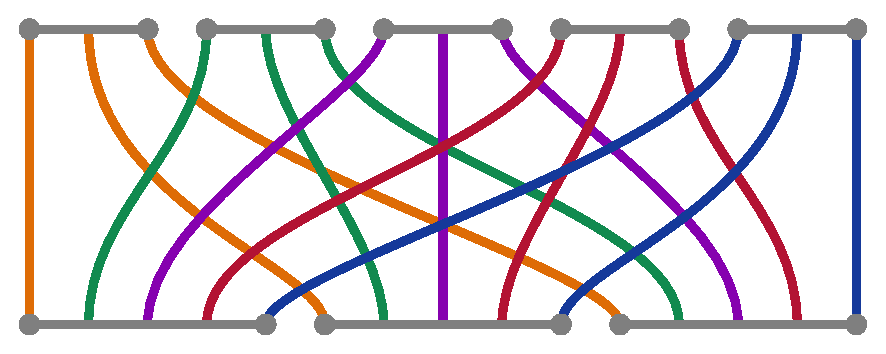
\includegraphics[width=0.8\columnwidth]{4-monoidal_structures/t-5-3.pdf}
% \end{figure}
% We now give sufficient conditions for equipping the $2$-monad $\underline{P}$ associated to a $\Lambda$-operad $P$ with a pseudo-commutative structure. Let $\mathbb{N}_{+}$ denote the set of positive natural numbers.

We now define what it means for a $\Lambda$-operad to be pseudo-commuative, before then showing that such an operad yields a pseudo-commutative structure on the corresponding $2$-monad $\underline{P}$. 

\begin{nota}
Let $\mathbb{N}_{+}$ denote the set of positive integers.
\end{nota}

\ngnoteil{Need to look back at how we structured other definitions, make it consistent}
\begin{Defi}\label{def:ps-comm_operad}
Let $P$ be a $\Lambda$-operad in $\mb{Cat}$. A pseudo-commutative structure on $P$ consists of the following data.
\ngnoteil{From before: QQQ Rewrite all this using the beta and delta operations, so it's consistent with before. This seems to be partially done, but need to recheck details}
    \begin{itemize}
        \item For each pair $(m,n) \in \mathbb{N}_{+}^2$, an element $t_{m,n} \in \Lambda(mn)$ such that $\pi(t_{m,n}) = \tau_{m,n}$.
        \item For each $p \in P(n)$, $q \in P(m)$, a natural isomorphism\ngnote{natural where/how?}
            \[
                \lambda_{p,q} \colon \mu(p;q,\ldots,q) \cdot t_{m,n} \cong \mu(q;p,\ldots,p).
            \]
            We write this as $\lambda_{p,q}\colon \mu(p; \underline{q}) \cdot t_{m,n} \cong \mu(q; \underline{p})$.
    \end{itemize}
These are required to satisfy the following axioms:  
    \begin{enumerate}
        \item\label{axiom:t_id} For all $n \in \mathbb{N}_+$,
            \[
                t_{1,n} = e_n = t_{n,1}
            \]
             and for all $p \in P(n)$, the isomorphism $\lambda_{p, \id}\colon p \cdot e_n \cong p$ is the identity map.
        % \item\label{axiom:t_equiv} QQQ Equivariance axiom - we decided this was just naturality in the end! (See Remark 11.2 in \cite{guillou_multiplicative}.) QQQ It's basically `compose, act, switch' is the same as `compose, switch, act', but can't actually see where it's used in the proof:
        %   \[
        %     \lambda_{p \cdot g, q \cdot h} \circ \mu^P\left(\id_p \cdot g; \underline{\id_q \cdot h}\right) = \mu^P\left(\id_q \cdot h; \underline{\id_p \cdot g}\right) \circ \lambda_{p,q}.
        %   \]
        % For each $p \in P(n)$, $q \in P(m)$, $g \in \Lambda(n)$, and $h \in \Lambda(m)$, the following diagram commutes:
        %   \[
        %     \xy
        %       (-20,10)*+{\mu^P\left(p;\underline{q}\right) \cdot t_{m,n}}="a";
        %       (20,10)*+{\mu^P\left(q;\underline{p}\right)}="b";
        %       (-20,-10)*+{\mu^P\left(p \cdot g; \underline{q \cdot h}\right) \cdot t_{m,n}}="c";
        %       (20,-10)*+{\mu^P\left(q \cdot h; \underline{p \cdot g}\right)}="d";
        %       %
        %       {\ar^{\lambda_{p,q}} "a" ; "b"};
        %       {\ar^{\mu^P\left(\id_q \cdot h; \underline{\id_p \cdot g}\right)} "b" ; "d"};
        %       {\ar_{\mu^P\left(\id_p \cdot g; \underline{\id_q \cdot h}\right) \cdot t_{m,n}} "a" ; "c"};
        %       {\ar_{\lambda_{p \cdot g, q \cdot h}} "c" ; "d"};
        %     \endxy
        %   \]
        \item\label{axiom:t_sumR} For all $l, m_1, \ldots, m_l, n \in \mathbb{N}_+$, with $M = \Sigma m_i$,
            \[
                \mu^{\Lambda}\left(e_l; t_{m_1,n}, \ldots, t_{m_l,n}\right) \cdot \mu^{\Lambda}\left(t_{l,n};\underline{e_{m_1},\ldots,e_{m_l}}\right) = t_{n,M}.
            \]
            \acnoteil{check below is same as above, then delete above}
            \[
              \beta(t_{n,m_1},\ldots,t_{n,m_l}) \cdot \delta_{\underline{m_i},\ldots,\underline{m_i}}(t_{n,l}) = t_{n,M}.
            \]
            Here $\underline{e_{m_1},\ldots,e_{m_l}}$ is the list $e_{m_{1}}, \ldots, e_{m_{l}}$ repeated $n$ times.
        \item\label{axiom:t_sumL} For all $l, m, n_1,\ldots, n_m \in \mathbb{N}_+$, with $N = \Sigma n_i$,
            \[
                \mu^{\Lambda}\left(t_{m,l};\underline{e_{n_1}},\ldots,\underline{e_{n_m}}\right) \cdot \mu^{\Lambda}\left(e_m;t_{n_1,l},\ldots,t_{n_m,l}\right) = t_{N,l}.
            \]
            \acnoteil{check below is same as above, then delete above}
            \[
              \delta_{\underline{n_1},\ldots,\underline{n_m}}(t_{m,l}) \cdot \beta(t_{n_1,l},\ldots,t_{n_m,l}) = t_{N,l}.
            \]
            Here $\underline{e_{n_{i}}}$ indicates that each $e_{n_{i}}$ is repeated $l$ times.
        \item\label{axiom:t_diagR} For any $l, m_i, n \in \mathbb{N}_+$, with $1 \leq i \leq n$, and $p \in P(l)$, $q_i \in P(m_i)$ and $r \in P(n)$, the following diagram commutes. (Note that we maintain the convention that anything underlined indicates a list, and double underlining indicates a list of lists. Each instance should have an obvious meaning from context and the equations appearing above.)
          \[
            \xy
                (0,0)*+{\mu\left(p;\underline{\mu(q_i;\underline{r})}\right) \cdot \mu(e_l;\underline{t_{n,m_i}})\mu(t_{n,l};\underline{\underline{e_{m_i}}})}="00";
                (60,0)*+{\mu\left(p;\underline{\mu(q_i;\underline{r})}\right) \cdot t_{n,M}}="10";
                (0,-15)*+{\mu\left(p;\underline{\mu(q_i;\underline{r})\cdot t_{n,m_i}}\right) \cdot \mu(t_{n,l};\underline{e_{m_1},\ldots,e_{m_l}})}="01";
                (60,-20)*+{\mu\left(\mu(p;q_1,\ldots,q_n);\underline{\underline{r}}\right)\cdot t_{n,M}}="11";
                (0,-30)*+{\mu\left(p;\underline{\mu(r;\underline{q_i})}\right) \cdot \mu(t_{n,l};\underline{e_{m_1},\ldots,e_{m_l}})}="02";
                (60,-40)*+{\mu\left(\mu(p;q_1,\ldots,q_n);\underline{\underline{r}}\right)}="12";
                (0,-45)*+{\mu\left(\mu(p;\underline{r}) \cdot t_{n,l} ; \underline{q_1,\ldots,q_n}\right)}="03";
                (60,-60)*+{\mu\left(r;\underline{\mu(p;q_1,\ldots,q_n)}\right)}="13";
                (0,-60)*+{\mu\left(\mu(r;\underline{p});\underline{q_1,\ldots,q_n}\right)}="04";
                {\ar@{=} "00" ; "10"};
                {\ar@{=} "00" ; "01"};
                {\ar@{=} "10" ; "11"};
                {\ar_{\mu(1;\underline{\lambda_{q_i,r}}) \cdot 1} "01" ; "02"};
                {\ar@{=} "02" ; "03"};
                {\ar@{=} "04" ; "13"};
                {\ar_{\mu(\lambda_{p,r};1)} "03" ; "04"};
                {\ar^{\lambda_{\mu(p;q_1,\ldots,q_n),r}} "11" ; "12"};
                {\ar@{=} "12" ; "13"};
            \endxy
          \]
        \item\label{axiom:t_diagL} For any $l,m, n_i \in \mathbb{N}_+$, with $1 \leq i \leq m$, and $p \in P(l)$, $q \in P(m)$ and $r_i \in P(n_i)$, the following diagram commutes.
          \[
            \xy
                (0,0)*+{\mu\left(\mu(p;\underline{q}) \cdot t_{m,l} ; \underline{\underline{r_i}}\right) \cdot \mu(e_m;\underline{t_{n_i,l}})}="00";
                (60,0)*+{\mu\left(\mu(p;\underline{q});\underline{\underline{r_i}}\right) \cdot \mu(t_{m,l};\underline{\underline{e_{n_i}}})\mu(e_{m};\underline{t_{n_i,l}})}="10";
                (60,-15)*+{\mu\left(p;\underline{\mu(q;\underline{r_i})}\right) \cdot \mu(t_{m,l};\underline{\underline{e_{n_i}}})\mu(e_{m};\underline{t_{n_i,l}})}="11";
                (0,-20)*+{\mu\left(\mu(q;\underline{p}); \underline{r_1},\ldots,\underline{r_m}\right) \cdot \mu(e_m;\underline{t_{n_i,l}})}="01";
                (0,-40)*+{\mu\left(q;\underline{\underline{\mu(p;r_i)}}\right) \cdot \mu(e_m;\underline{t_{n_i,l}})}="02";
                (0,-60)*+{\mu\left(q;\underline{\mu(p;\underline{r_i}) \cdot t_{n_i,l}}\right)}="03";
                (60,-30)*+{\mu\left(p;\underline{\mu(q;r_1,\ldots,r_m)}\right) \cdot t_{N,l}}="12";
                (60,-45)*+{\mu\left(\mu(q;r_1,\ldots,r_m); \underline{\underline{p}}\right)}="13";
                (60,-60)*+{\mu\left(q;\underline{\mu(r_i;\underline{p})}\right)}="14";
                {\ar@{=} "00" ; "10"};
                {\ar@{=} "10" ; "11"};
                {\ar@{=} "11" ; "12"};
                {\ar^{\lambda_{p,\mu(q;r_1,\ldots,r_m)}} "12" ; "13"};
                {\ar@{=} "13" ; "14"};
                {\ar_{\mu(\lambda_{p,q};1) \cdot 1} "00" ; "01"};
                {\ar@{=} "01" ; "02"};
                {\ar@{=} "02" ; "03"};
                {\ar_{\mu(1;\underline{\lambda_{p,r_i}})} "03" ; "14"};
            \endxy
          \]
    \end{enumerate}
\end{Defi}

\begin{remark}
Remark 11.2 of \cite{guillou_multiplicative} describes the need for an extra equivariance axiom in the pseudo-commutative structure definition, some detail of which is also described in \cite{guillou_symmetric}. We also believed this to be true until a realisation that the equivariance axiom of \cite{guillou_multiplicative}[11.1, Axiom (iii)] becomes the following requirement:
          \[
            \lambda_{p \cdot g, q \cdot h} \circ \left(\mu^P\left(\id_p \cdot g; \underline{\id_q \cdot h}\right) \cdot t_{m,n}\right) = \mu^P\left(\id_q \cdot h; \underline{\id_p \cdot g}\right) \circ \lambda_{p,q}.
          \]
On closer inspection, this equation is an instance of naturality for $\lambda$, as shown in the naturality square below.\ngmpar{What are the morphisms $p \to p \cdot g$ that this is naturality wrt? Probably the unique $e \to g$ acting on $p$, but we should explain.}
          \[
            \xy
              (-20,10)*+{\mu^P\left(p;\underline{q}\right) \cdot t_{m,n}}="a";
              (20,10)*+{\mu^P\left(q;\underline{p}\right)}="b";
              (-20,-10)*+{\mu^P\left(p \cdot g; \underline{q \cdot h}\right) \cdot t_{m,n}}="c";
              (20,-10)*+{\mu^P\left(q \cdot h; \underline{p \cdot g}\right)}="d";
              %
              {\ar^{\lambda_{p,q}} "a" ; "b"};
              {\ar^{\mu^P\left(\id_q \cdot h; \underline{\id_p \cdot g}\right)} "b" ; "d"};
              {\ar_{\mu^P\left(\id_p \cdot g; \underline{\id_q \cdot h}\right) \cdot t_{m,n}} "a" ; "c"};
              {\ar_{\lambda_{p \cdot g, q \cdot h}} "c" ; "d"};
            \endxy
          \]
\end{remark}

\begin{thm}\label{thm:pscomm}
Let $P$ be a $\Lambda$-operad in $\mb{Cat}$ equipped with a pseudo-commutative structure. Then $\underline{P}$ has a pseudo-commutativity.
\end{thm}

% \begin{thm}\label{pscomm}
% Let $P$ be a $\Lambda$-operad. Then the following equip $\underline{P}$ with a pseudo-commutative structure.
%     \begin{itemize}
%         \item For each pair $(m,n) \in \mathbb{N}_{+}^2$, we are given an element $t_{m,n} \in \Lambda(mn)$ such that $\pi(t_{m,n}) = \tau_{m,n}$.
%         \item For each $p \in P(n)$, $q \in P(m)$, we are given a natural isomorphism
%             \[
%                 \lambda_{p,q} \colon \mu(p;q,\ldots,q) \cdot t_{m,n} \cong \mu(q;p,\ldots,p).
%             \]
%             We write this as $\lambda_{p,q}\colon \mu(p; \underline{q}) \cdot t_{m,n} \cong \mu(q; \underline{p})$.
%     \end{itemize}
% These must satisfy the following:  
%     \begin{enumerate}
%         \item For all $n \in \mathbb{N}_+$\nomenclature[N]{$\mathbb{N}_+$}{the set of positive natural numbers},
%             \[
%                 t_{1,n} = e_n = t_{n,1}
%             \]
%              and for all $p \in P(n)$, the isomorphism $\lambda_{p, \id}\colon p \cdot e_n \cong p$ is the identity map.
%         \item For all $l, m_1, \ldots, m_l, n \in \mathbb{N}_+$, with $M = \Sigma m_i$,
%             \[
%                 \mu^{\Lambda}\left(e_l; t_{m_1,n}, \ldots, t_{m_l,n}\right) \cdot \mu^{\Lambda}\left(t_{l,n};\underline{e_{m_1},\ldots,e_{m_l}}\right) = t_{n,M}.
%             \]
%             Here $\underline{e_{m_1},\ldots,e_{m_l}}$ is the list $e_{m_{1}}, \ldots, e_{m_{l}}$ repeated $n$ times.
%         \item For all $l, m, n_1,\ldots, n_m \in \mathbb{N}_+$, with $N = \Sigma n_i$,
%             \[
%                 \mu^{\Lambda}\left(t_{m,l};\underline{e_{n_1}},\ldots,\underline{e_{n_m}}\right) \cdot \mu^{\Lambda}\left(e_m;t_{n_1,l},\ldots,t_{n_m,l}\right) = t_{N,l}.
%             \]
%             Here $\underline{e_{n_{i}}}$ indicates that each $e_{n_{i}}$ is repeated $l$ times.
%         \item For any $l, m_i, n \in \mathbb{N}_+$, with $1 \leq i \leq n$, and $p \in P(l)$, $q_i \in P(m_i)$ and $r \in P(n)$, the following diagram commutes. (Note that we maintain the convention that anything underlined indicates a list, and double underlining indicates a list of lists. Each instance should have an obvious meaning from context and the equations appearing above.)
%           \[
%             \xy
%                 (0,0)*+{\mu\left(p;\underline{\mu(q_i;\underline{r})}\right) \cdot \mu(e_l;\underline{t_{n,m_i}})\mu(t_{n,l};\underline{\underline{e_{m_i}}})}="00";
%                 (60,0)*+{\mu\left(p;\underline{\mu(q_i;\underline{r})}\right) \cdot t_{n,M}}="10";
%                 (0,-15)*+{\mu\left(p;\underline{\mu(q_i;\underline{r})\cdot t_{n,m_i}}\right) \cdot \mu(t_{n,l};\underline{e_{m_1},\ldots,e_{m_l}})}="01";
%                 (60,-20)*+{\mu\left(\mu(p;q_1,\ldots,q_n);\underline{\underline{r}}\right)\cdot t_{n,M}}="11";
%                 (0,-30)*+{\mu\left(p;\underline{\mu(r;\underline{q_i})}\right) \cdot \mu(t_{n,l};\underline{e_{m_1},\ldots,e_{m_l}})}="02";
%                 (60,-40)*+{\mu\left(\mu(p;q_1,\ldots,q_n);\underline{\underline{r}}\right)}="12";
%                 (0,-45)*+{\mu\left(\mu(p;\underline{r}) \cdot t_{n,l} ; \underline{q_1,\ldots,q_n}\right)}="03";
%                 (60,-60)*+{\mu\left(r;\underline{\mu(p;q_1,\ldots,q_n)}\right)}="13";
%                 (0,-60)*+{\mu\left(\mu(r,\underline{p});\underline{q_1,\ldots,q_n}\right)}="04";
%                 {\ar@{=} "00" ; "10"};
%                 {\ar@{=} "00" ; "01"};
%                 {\ar@{=} "10" ; "11"};
%                 {\ar_{\mu(1;\underline{\lambda_{q_i,r}}) \cdot 1} "01" ; "02"};
%                 {\ar@{=} "02" ; "03"};
%                 {\ar@{=} "04" ; "13"};
%                 {\ar_{\mu(\lambda_{p,r};1)} "03" ; "04"};
%                 {\ar^{\lambda_{\mu(p;q_1,\ldots,q_n),r}} "11" ; "12"};
%                 {\ar@{=} "12" ; "13"};
%             \endxy
%           \]
%         \item For any $l,m, n_i \in \mathbb{N}_+$, with $1 \leq i \leq m$, and $p \in P(l)$, $q \in P(m)$ and $r_i \in P(n_i)$, the following diagram commutes.
%           \[
%             \xy
%                 (0,0)*+{\mu\left(\mu(p;\underline{q}) \cdot t_{m,l} ; \underline{\underline{r_i}}\right) \cdot \mu(e_m;\underline{t_{n_i,l}})}="00";
%                 (60,0)*+{\mu\left(\mu(p;\underline{q});\underline{\underline{r_i}}\right) \cdot \mu(t_{m,l};\underline{\underline{e_{n_i}}})\mu(e_{m};\underline{t_{n_i,l}})}="10";
%                 (60,-15)*+{\mu\left(p;\underline{\mu(q;\underline{r_i})}\right) \cdot \mu(t_{m,l};\underline{\underline{e_{n_i}}})\mu(e_{m};\underline{t_{n_i,l}})}="11";
%                 (0,-20)*+{\mu\left(\mu(q;\underline{p}); \underline{r_1},\ldots,\underline{r_m}\right) \cdot \mu(e_m;\underline{t_{n_i,l}})}="01";
%                 (0,-40)*+{\mu\left(q;\underline{\underline{\mu(p;r_i)}}\right) \cdot \mu(e_m;\underline{t_{n_i,l}})}="02";
%                 (0,-60)*+{\mu\left(q;\underline{\mu(p;\underline{r_i}) \cdot t_{n_i,l}}\right)}="03";
%                 (60,-30)*+{\mu\left(p;\underline{\mu(q;r_1,\ldots,r_m)}\right) \cdot t_{N,l}}="12";
%                 (60,-45)*+{\mu\left(\mu(q;r_1,\ldots,r_m); \underline{\underline{p}}\right)}="13";
%                 (60,-60)*+{\mu\left(q;\underline{\mu(r_i;\underline{p})}\right)}="14";
%                 {\ar@{=} "00" ; "10"};
%                 {\ar@{=} "10" ; "11"};
%                 {\ar@{=} "11" ; "12"};
%                 {\ar^{\lambda_{p,\mu(q;r_1,\ldots,r_m)}} "12" ; "13"};
%                 {\ar@{=} "13" ; "14"};
%                 {\ar_{\mu(\lambda_{p,q};1) \cdot 1} "00" ; "01"};
%                 {\ar@{=} "01" ; "02"};
%                 {\ar@{=} "02" ; "03"};
%                 {\ar_{\mu(1;\underline{\lambda_{p,r_i}})} "03" ; "14"};
%             \endxy
%           \]
%     \end{enumerate}
% \end{thm}

\begin{proof}
\ngnoteil{go through details again}
We refer to the Axioms in \cref{def:ps-comm_operad} throughout. We begin the proof by defining an invertible modification $\gamma$ for the pseudo-commutativity for which the components are natural transformations $\gamma_{A,B}$. Such a transformation $\gamma_{A,B}$ has components with source
  \[
    \left[\mu\left(p; \underline{q}\right); \underline{(a, \underline{b})}\right]
  \]
and target
  \[
    \left[\mu\left(q; \underline{p}\right); \underline{(\underline{a},b)}\right].
  \]
Now $ \lambda_{p,q} \colon \mu(p;q,\ldots,q) \cdot t_{m,n} \cong \mu(q;p,\ldots,p)$ gives rise to another map by multiplication on the right by $t_{m,n}^{-1}$,
  \[
    \lambda_{p,q}\cdot t_{m,n}^{-1} \colon \mu(p;q,\ldots,q) \cong \mu(q;p,\ldots,p) \cdot t_{m,n}^{-1},
  \]
so we define $(\gamma_{A,B})_{[p;a_1,\ldots,a_n],[q;b_1,\ldots,b_m]}$ to be the morphism which is the image of $(\lambda_{p,q}\cdot t_{m,n}^{-1}, 1)$ under the map
  \[
    \coprod P(n) \times (A \times B)^{n} \rightarrow \coprod \coeq{P}{A \times B}{\Lambda}{n}.
  \]
Naturality of $\gamma_{A,B}$ follows from that of each $\lambda_{p,q}$. We will write this morphism as $[\lambda_{p,q}t_{m,n}^{-1}, 1]$. In the case that either $p$ or $q$ is an identity then we choose the component of $\gamma$ to be the isomorphism involving the appropriate identity element using Axiom \ref{axiom:t_id} above.

There are two things to note about the definition above before we continue. First, it is easy to check that
  \[
    t_{m,n}^{-1} \cdot \underline{\left(a, \underline{b}\right)} = \underline{\left(\underline{a},b\right)}
  \]
since $\pi(t_{m,n}) = \tau_{m,n}$; this ensures that $\gamma$ has the correct target. Second, the morphism above has second component the identity. This is actually forced upon us by the requirement that $\gamma$ be a modification:  in the case that $A,B$ are discrete categories, the only possible morphism is an identity, and the modification axiom then forces that statement to be true for general $A,B$ by considering the inclusion $A_{0} \times B_{0} \hookrightarrow A \times B$ where $A_{0}, B_{0}$ are the discrete categories with the same objects as $A, B$.

We show that this is a modification by noting that it does not rely on objects in the lists $a_1, \ldots, a_n$ or $b_1, \ldots, b_m$, only on their lengths and the operations $p$ and $q$. As a result, if there are functors $f \colon A \rightarrow A'$ and $g \colon B \rightarrow B'$, then it is clear that
    \[
        (\underline{P}(f\times g) \circ \gamma_{A,B})_{\left[p;\underline{a}\right],\left[q;\underline{b}\right]} = [\lambda_{p,q},\underline{1}] = (\gamma_{A',B'} \circ (\underline{P}f\times \underline{P}g))_{\left[p;\underline{a}\right],\left[q;\underline{b}\right]}.
    \]
As such we can simply write $(\gamma_{A,B})_{[p;\underline{a}],[q;\underline{b}]}$ in shorthand as $\gamma_{p,q}$.

There are now seven axioms to check for a pseudo-commutativity:  three strength axioms, two unit axioms, and two multiplication axioms. For the first strength axiom, we must verify that two different $2$-cells of shape
  \[
    \xy
      (0,0)*+{A \times TB \times TC}="0";
      (50,0)*+{T(A \times B \times C)}="1";
      {\ar@/^1pc/ "0"; "1"};
      {\ar@/_1pc/ "0"; "1"};
      (25,0)*{\Downarrow}
    \endxy
  \]
are equal. The first of these is $\gamma$ precomposed with $d \times 1$, and so is the component of $\gamma$ at an object
  \[
    \left( [p;(a,b_1),\ldots,(a,b_n)], [q; c_{1}, \ldots, c_{m}] \right).
  \]
The second of these is $d$ applied to the component of $1 \times \gamma$ at
  \[
    \left(a, ([p;b_1,\ldots,b_n], [q; c_{1}, \ldots, c_{m}]) \right).
  \]
It is straightforward to compute that each of these maps is the image of $\left(\lambda_{p,q}\cdot t_{m,n}^{-1},1\right)$ under the functor
  \[
    \coprod P(n) \times (A \times B)^{n} \rightarrow \coprod \coeq{P}{A \times B}{\Lambda}{n}.
  \]
The other two strength axioms follow by analogous calculations for other whiskerings of $\gamma$ with $d$ or $d^{*}$.

For the unit axioms, we must compute the components of $\gamma$ precomposed with $\eta \times 1$ for the first axiom and $1 \times \eta$ for the second. Thus for the first unit axiom, we must compute the component of $\gamma$ at $\left( [e;a], [p; b_{1}, \ldots, b_{m}] \right)$. By definition, this is the image of $(\lambda_{e,p}\cdot t^{-1}_{m,1}, 1)$ under the map to the coequalizer, and by Axiom \ref{axiom:t_id} of \ref{def:ps-comm_operad} know that $t^{-1}_{m,1}$ is the identity element and this isomorphism is the identity as well, so this component of $\gamma$ is also the identity. The second unit axiom follows similarly, using that $t^{-1}_{1,n}$ is the identity.

For the multiplication axioms, first note that Axiom \ref{axiom:t_sumR} is necessary in order to ensure the existence of the top horizontal equality in the diagram of Axiom \ref{axiom:t_diagR} for the pseudo-commutative structure; the same goes for Axioms \ref{axiom:t_sumL} and \ref{axiom:t_diagL}. We now explain how Axioms \ref{axiom:t_sumR} and \ref{axiom:t_diagR} for the pseudo-commutative structure ensure that the first multiplication axiom holds, with the same reasoning showing that Axioms \ref{axiom:t_sumL} and \ref{axiom:t_diagL} imply the second multiplication axiom.

We begin by studying the pasting diagram in the first multiplication axiom, but computing its values using the strength and costrength for the non-symmetric operad underlying $P$; this means that we evaluate on objects of the form $(p; a_{1}, \ldots, a_{n})$ rather than on their equivalence classes. Let $p \in P(l), q_{i} \in P(m_{i})$ for $1 \leq i \leq l$, and $r \in P(n)$. Computing the top and right leg around the pasting diagram gives the function on objects which sends
  \[
    \left( (p; (q_{1}; \un{a_{1}}), \ldots, (q_{l}; \un{a_{l}})), (r; \un{b}) \right)
  \]
to
  \[
    \left( \mu(p; \mu(q_{1}; \un{r}), \ldots, \mu(q_{l}; \un{r})); (\un{(a_{1\bullet}, \un{b})}), \ldots, (\un{(a_{l\bullet}, \un{b})}) \right),
  \]
where $(\un{(a_{i\bullet}, \un{b})})$ is the list of pairs
  \[
    (a_{i1}, b_{1}), \ldots, (a_{i1}, b_{m}), (a_{i2}, b_{1}), \ldots, (a_{in_{i}}, b_{m}).
  \]
Then $\un{P}\gamma$ is the image of the morphism which is the identity on the $(a_{ij}, b_{k})$'s, and is the morphism
  \[
    \mu\left(1;\lambda_{q_1,r}t^{-1}_{n,m_1},\ldots,\lambda_{q_l,r}t^{-1}_{n,m_l}\right)
  \]
on the first component with domain and codomain shown below.
  \[
    \mu\left(p;\mu\left(q_1;\un{r}\right),\ldots,\mu\left(q_n;\un{r}\right)\right) \longrightarrow \mu\left(p;\mu\left(r;\un{q_1}\right)t^{-1}_{n,m_1},\ldots,\mu\left(r;\un{q_l}\right)t^{-1}_{n,m_l}\right)
  \]
% \[
% \xy
% {\ar^{\scriptstyle \mu\left(1; \lambda_{q_{1}, r} t^{-1}_{n,m_{1}}, \ldots, \lambda_{q_{1}, r} t^{-1}_{n,m_{l}}\right)} (0,0)*+{\scriptstyle \mu\left(p; \mu(q_{1}; \un{r}), \ldots, \mu(q_{n}; \un{r})\right)}; (75,0)*+{\scriptstyle \mu\left(p; \mu(r; \un{q_{1}}) t^{-1}_{n,m_{1}}, \ldots, \mu(r; \un{q_{l}}) t^{-1}_{n,m_{l}} \right)} }
% \endxy
% \]
% on the first component. 
By the $\Lambda$-operad axioms, the target of this morphism is equal to
  \[
    \mu\left(p; \mu\left(r; \un{q_{1}}\right), \ldots, \mu\left(r; \un{q_{l}}\right) \right)\mu\left(e_{l}; t^{-1}_{n,m_{1}}, \ldots, t^{-1}_{n,m_{l}}\right).
  \]
Note that this is not the same object as one obtains by computing $T\mu \circ T^{2}d^{*} \circ Td \circ d^{*}$ using the underlying non-symmetric operad of $P$ as we are required to use the $\Lambda$-equivariance to ensure that the target of $\gamma$ is the correct one.

Next we compute the source of $(\mu \circ Td^{*})*\gamma$, the other $2$-cell in the pasting appearing in the first multiplication axiom. We compute this once again using the strength and costrength for the underlying non-symmetric operad, and note once again that this will not match our previous calculations precisely, but only up to an application of $\Lambda$-equivariance. This functor has its map on objects given by
  \[
    \left( (p; (q_{1}; \un{a_{1}}), \ldots, (q_{l}; \un{a_{l}})), (r; \un{b}) \right) \mapsto \left(\mu(\mu(p; \un{r}); \un{q_{1}}, \ldots, \un{q_{l}}); \un{(\un{a_{1}}, b_{\bullet})}, \ldots, \un{(\un{a_{l}}, b_{\bullet})} \right).
  \]
  Note that if we apply $\Lambda$-equivariance, this matches the target computed above. Once again the component of $\gamma$ is the image of a morphism which is the identity on the $(a_{ij}, b_{k})$'s, and its first component is
  \[
    \xy
      {\ar^{\mu\left(\lambda_{p,r} \cdot t^{-1}_{n,l}; 1, \ldots, 1\right)} (0,0)*+{\mu\left(\mu(p; \un{r}); \un{q_{1}}, \ldots, \un{q_{l}}\right)}; (60,0)*+{\mu\left(\mu(r; \un{p})\cdot t^{-1}_{n,l}; \un{q_{1}}, \ldots, \un{q_{l}}\right).} }
    \endxy
  \]

We cannot compose these morphisms in $\coprod P(n) \times (A \times B)^{n}$ as they do not have matching source and target, but we can in $\coprod P(n) \times_{\Lambda} (A \times B)^{n}$. The resulting morphism has first component given by the image of
  \[
    \xy
      {\ar^{\scriptstyle \mu\left(1; \lambda_{q_{1}, r} t^{-1}_{n,m_{1}}, \ldots, \lambda_{q_{1}, r} t^{-1}_{n,m_{l}}\right)} (0,0)*+{\scriptstyle \mu\left(p; \mu\left(q_{1}; \un{r}\right), \ldots, \mu\left(q_{n}; \un{r}\right)\right)}; (75,0)*+{\scriptstyle \mu\left(p; \mu\left(r; \un{q_{1}}\right) t^{-1}_{n,m_{1}}, \ldots, \mu\left(r; \un{q_{l}}\right) t^{-1}_{n,m_{l}} \right)} };
      {\ar^<<<<<<<<<<<<<<<<<<<<<<{\scriptstyle \mu\left(\lambda_{p,r} \cdot t^{-1}_{n,l}; 1, \ldots, 1\right)\cdot \mu\left(e_{l}; t^{-1}_{n,m_{1}}, \ldots, t^{-1}_{n,m_{l}}\right)} (0,-10)*+{}; (75,-10)*+{\scriptstyle \mu\left(\mu\left(r; \un{p}\right)\cdot t^{-1}_{n,l}; \un{q_{1}}, \ldots, \un{q_{l}}\right)\cdot \mu\left(e_{l}; t^{-1}_{n,m_{1}}, \ldots, t^{-1}_{n,m_{l}}\right),} }
    \endxy
  \]
where we have made use of the operad axioms in identifying the target of the first map with the source of the second. Using the $\Lambda$-operad axioms again on the target, we find that
  \[
    \mu\left(\mu(r; \un{p})\cdot t^{-1}_{n,l}; \un{q_{1}}, \ldots, \un{q_{l}}\right)\cdot \mu(e_{l}; t^{-1}_{n,m_{1}}, \ldots, t^{-1}_{n,m_{l}})
  \]
is equal to
  \[
    \mu\left(\mu(r; \un{p}); \un{q_{1}, \ldots, q_{l}}\right) \cdot \mu(t^{-1}_{n,l}; \un{e}) \cdot \mu(e_{l}; t^{-1}_{n,m_{1}}, \ldots, t^{-1}_{n,m_{l}}).
  \]
This composite of two morphisms, together with the necessary identities coming from operad axioms, is precisely the left and bottom leg of the diagram in Axiom \ref{axiom:t_diagR}. Using the same method, one then verifies that $\gamma * (\mu \times 1)$ has its first component the image of the morphism appearing along the top and right leg of the diagram in \ref{axiom:t_diagR}. The second component of these morphisms are all identities arising from $\Lambda$-equivariance, so the first multiplication axiom is a consequence of Axioms \ref{axiom:t_sumR} and \ref{axiom:t_diagR} for the pseudo-commutative structure. We leave the calculations for the second multiplication axiom to the reader as they are of the same nature, using Axioms \ref{axiom:t_sumL} and \ref{axiom:t_diagL}.
\end{proof}

\begin{cor}\label{cor:not-pc}
Let $P$ be a non-symmetric operad. Then the induced monad $\underline{P}$ is never pseudo-commutative.
\end{cor}
\begin{proof}
\ngnoteil{go through details again}
In the non-symmetric case, the $2$-monad is just given using coproducts and products, i.e., there is no coequalizer. In order to define $\gamma$, we then need an isomorphism
  \[
    \left(\mu(p; \underline{q}); \underline{(a, \underline{b})}\right) \cong \left(\mu(q; \underline{p}); \underline{(\underline{a},b)}\right).
  \]
When $A,B$ are discrete, there is no isomorphism $\underline{\left(a,\underline{b}\right)} \cong \underline{\left(\underline{a},b\right)}$, and therefore no such $\gamma$ can exist.
\end{proof}



Hyland and Power also define a symmetry for a pseudo-commutative structure on a $2$-monad $T$. This symmetry is then reflected in the monoidal structure on the $2$-category of algebras, which will then also have a symmetric tensor product (in a suitable, $2$-categorical sense)\ngnote{include specific reference}.
\acnote{This is prop 18 in HP. But they are talking about the \emph{multicategory} $T$-Alg.}
\begin{Defi}
Let $T \colon \m{K} \rightarrow \m{K}$ be a $2$-monad on a symmetric monoidal $2$-category $\m{K}$ with symmetry $c$. We then say that a pseudo-commutativity $\gamma$ for $T$ is \textit{symmetric} when the following is satisfied for all $A$, $B \in \m{K}$:
    \[
        Tc_{A,B} \circ \gamma_{A,B} \circ c_{TB, TA} = \gamma_{B,A}.
    \]
\end{Defi}

With the notion of symmetry at hand we are able to extend the above theorem, stating when $\underline{P}$ is symmetric.
\begin{thm}
The pseudo-commutativity of $\underline{P}$ given by \cref{pscomm}  is symmetric if for all $m,n \in \mathbb{N}_+$ the two conditions below hold.
    \begin{enumerate}
        \item $t_{m,n} = t_{n,m}^{-1}$.
        \item The following diagram commutes:
          \[
              \xy
                (0,0)*+{\mu\left(p;\underline{q}\right) \cdot t_{m,n}t_{n,m}}="00";
                (30,0)*+{\mu\left(p;\underline{q}\right) \cdot e_{mn}}="10";
                (0,-15)*+{\mu\left(q;\underline{p}\right) \cdot t_{n,m}}="01";
                (30,-15)*+{\mu\left(p;\underline{q}\right)}="11";
                {\ar@{=} "00" ; "10"};
                {\ar_{\lambda_{p,q} \cdot 1} "00" ; "01"};
                {\ar@{=} "10" ; "11"};
                {\ar_{\lambda_{q,p}} "01" ; "11"};
              \endxy
          \]
    \end{enumerate}
\end{thm}
\begin{proof}
The commutativity of the diagram above ensures that the first component of the symmetry axiom commutes in $P(n)$ before taking equivalence classes in the coequalizer, just as in the proof of \cref{pscomm}.
\end{proof}

\begin{Defi}
Let $P$ be a $\Lambda$-operad in $\mb{Cat}$. We say that $P$ is \textit{contractible} if each category $P(n)$ is equivalent to the terminal category.
\end{Defi}

\begin{cor}\label{cor:contract-to-psc}
If $P$ is contractible and there exist $t_{m,n}$ as in \cref{pscomm}, then $\underline{P}$ acquires a pseudo-commutativity. Furthermore, it is symmetric if $t_{n,m} = t_{m,n}^{-1}$.
\end{cor}
\begin{proof}
The only thing left to define is the collection of natural isomorphisms $\lambda_{p,q}$. But since each $P(n)$ is contractible, $\lambda_{p,q}$ must be the unique isomorphism between its source and target, and furthermore the last two axioms hold since any pair of parallel arrows are equal in a contractible category.
\end{proof}

\begin{cor}\label{cor:contractplussym-to-psc}
If $P$ is a contractible symmetric operad then $\underline{P}$ has a symmetric pseudo-commutativity.
\end{cor}
\begin{proof}
We choose $t_{m,n} = \tau_{m,n}$.
\end{proof}

\begin{rem}\label{rem:symm-and-contract}
If a $\Lambda$-operad $P$ is contractible, it is not the case that its symmetrization $S(P)$ (see \cref{thm_sym}) will also be contractible.
\ngnoteil{now just give an example, do braids work?}
Thus we see that a given $\Lambda$-operad $P$ might satisfy the hypotheses of \cref{cor:contract-to-psc} without its symmetrization $S(P)$ satisfying the hypotheses of \cref{cor:contractplussym-to-psc}.
\ngnoteil{This is exactly the kind of thing that ``keeping more complicated action operads around lets you do more stuff'' needs to reference!}

%The category $\coequ{P}{\Sigma}{\Lambda}{n}$ will necessarily be a groupoid as it is a colimit of groupoids: contractible categories are always groupoids, and both $\Lambda(n)$ and $\Sigma_{n}$ are discrete. Let $g \in \textrm{ker} \, \pi_{n}$ be any non-identity element, and let $p \in P(n)$ be any object. Then
%  \[
%    [p \cdot g, e] = [p, \pi(g)e] = [p,e],
%  \]
%but unless $p\cdot g = p$ in $P(n)$, there will be a unique isomorphism between them that will not be the identity, and hence will define a nontrivial automorphism of $[p,e]$ in  $\coequ{P}{\Sigma}{\Lambda}{n}$. The existence of such ensures that $\coequ{P}{\Sigma}{\Lambda}{n}$ is not contractible.
\end{rem}



\section{Extended Example: Coboundary Categories}\label{sec:exex-cactus}

\ngnoteil{This section could still move somewhere else. I have a presentation for the symmetric groups as an action operad in section 7, and this doesn't use much more than that.}

We now turn to an example that is not as widely known in the categorical literature, that of coboundary categories \cite{drin-quasihopf}. These arise in the representation theory of quantum groups and in the theory of crystals \cite{hk-cobound, hk-quantum}. Our goal here is to refine the relationship between coboundary categories and the operad of $n$-fruit cactus groups in \cite{hk-cobound} by using the theory of action operads\ngnote{I think in particular we want to do this via presentations} and our Borel construction. We begin by recalling the definition of a coboundary category.


\begin{Defi}\label{def:cobcat}
A \textit{coboundary category} is a monoidal category $C$ equipped with a natural isomorphism $\sigma_{x,y} \colon x \otimes y \rightarrow y \otimes x$ (called the \textit{commutor}) such that
\begin{itemize}
\item $\sigma_{y,x} \circ \sigma_{x,y} = 1_{x \otimes y}$ and
\item the diagram
  \[
    \xy
      (0,0)*+{(x \otimes y) \otimes z} ="00";
      (35,0)*+{x \otimes (y \otimes z)} ="10";
      (70,0)*+{x \otimes (z \otimes y)} ="20";
      (0,-15)*+{(y \otimes x) \otimes z} ="01";
      (35,-15)*+{z \otimes (y \otimes x)} ="11";
      (70,-15)*+{(z \otimes y )\otimes x} ="21";
      {\ar "00"; "10" };
      {\ar^{1 \sigma_{y,z}} "10"; "20" };
      {\ar^{\sigma_{x,zy}} "20"; "21" };
      {\ar_{\sigma_{x,y}1} "00"; "01" };
      {\ar_{\sigma_{yx,z}} "01"; "11" };
      {\ar "11"; "21" };
    \endxy
  \]
commutes (in which the unlabeled morphisms are an associator and an inverse associator).
\end{itemize}
\end{Defi}

\begin{example}\label{ex:cobcats}
\begin{enumerate}
\item As noted by Savage \cite{savage-braidcob}, any braiding automatically satisfies the cactus relation (the diagram in \cref{def:cobcat}). However, since braidings need not be involutions this does not mean that any braided monoidal category is a coboundary category. However, it should then be clear that any symmetric monoidal category is also a coboundary category.
\item The name coboundary category comes from the original work of Drinfeld \cite{drin-quasihopf} in which he shows that the category of representations of a coboundary Hopf algebra has the structure of coboundary category.
\item Henriques and Kamnitzer \cite{hk-cobound} show that the category of crystals for a finite dimensional complex reductive Lie algebra has the structure of a coboundary category. 
\end{enumerate}
\end{example}

\ngnoteil{replace what follows with a discussion/reference to \cref{thm:wlmc-to-lmc}}

Our interest is in strict coboundary categories by which we mean coboundary categories with strict underlying monoidal category. Under the assumption of strictness, the second axiom above does not include associations for the tensor product and reduces to a square. To show that every coboundary category is equivalent to a strict coboundary category, we must introduce the $2$-category $\mb{CobCat}$ of coboundary categories.

\begin{Defi}
Let $(C,\sigma), (C', \sigma')$ be coboundary categories. A \emph{coboundary functor} $F \colon C \rightarrow C'$ is a strong monoidal functor (with invertible constraints $\varphi_{0}$ for the unit and $\varphi_{x,y}$ for the tensor product) such that the following diagram commutes for all objects $x$, $y \in \m{C}$.
  \[
    \xy
      (0,0)*+{Fx \otimes Fy}="00";
      (25,0)*+{F(x \otimes y)}="10";
      (0,-20)*+{Fy \otimes Fx}="01";
      (25,-20)*+{F(y \otimes x)}="11";
      %
      {\ar^{\varphi_{x,y}} "00";"10"};
      {\ar^{F\sigma_{x,y}} "10";"11"};
      {\ar_{\sigma_{Fx,Fy}} "00";"01"};
      {\ar_{\varphi_{y,x}} "01";"11"};
    \endxy
  \]
  % \[
  %   F\sigma_{x,y} \circ \varphi_{x,y} = \varphi_{y,x} \circ \sigma_{Fx,Fy}'
  % \]
\end{Defi}

Coboundary functors are composed just as strong monoidal functors are, giving the following.

\begin{lem}
Coboundary categories, coboundary functors, and monoidal transformations form a $2$-category, which we denote $\mb{CobCat}$.
\end{lem}


\begin{prop}
Let $(C, \sigma)$ be a coboundary category. Then there exists a strict coboundary category $(C', \sigma')$ which is equivalent to $(C, \sigma)$ in $\mb{CobCat}$.
\end{prop}
\begin{proof}
Consider the underlying monoidal category of $(C, \sigma)$, which we will just write as $C$. We can find a strict monoidal category $C'$ by coherence for monoidal categories together with an equivalence, as monoidal categories, between $C$ and $C'$. By standard methods \cite{maclane-catwork}, this can be improved to an adjoint equivalence between $C$ and $C'$ in the $2$-category of monoidal categories, strong monoidal functors, and monoidal transformations. Let $F \colon  C \rightarrow C', G \colon C' \rightarrow C$ be the functors in this adjoint equivalence, and $\eta \colon 1 \Rightarrow FG$ the unit (which we note for emphasis is invertible since it the unit of an adjoint equivalence). For objects $x,y \in C'$, we define a commutor $\sigma'$ for $C'$ as the following composite.
  % \begin{align*}
  %   xy & \stackrel{\eta \otimes \eta}{\longrightarrow} FGxFGy \\
  %   & \stackrel{\cong}{\longrightarrow} F(GxGy) \\
  %   & \stackrel{F\sigma}{\longrightarrow} F(GyGx) \\
  %   & \stackrel{\cong}{\longrightarrow}  FGyFGx \\
  %   & \stackrel{\eta^{-1} \otimes \eta^{-1}}{\longrightarrow} yx.
  % \end{align*}
  % \begin{align*}
  %   xy &\xrightarrow{\eta \otimes \eta} FGxFGy \\
  %   &\xrightarrow{\cong} F(GxGy) \\
  %   &\xrightarrow{F\sigma} F(GyGx) \\
  %   &\xrightarrow{\cong} FGyFGx \\
  %   &\xrightarrow{\eta^{-1} \otimes \eta^{-1}} yx
  % \end{align*}
  \[
    xy \xrightarrow{\eta \otimes \eta} FGxFGy
    \xrightarrow{\cong} F(GxGy)
    \xrightarrow{F\sigma} F(GyGx)
    \xrightarrow{\cong} FGyFGx
    \xrightarrow{\eta^{-1} \otimes \eta^{-1}} yx
  \]
We then leave to the reader, if they wish, the computations to show that $\sigma'$ is a commutor for $C'$ and that $F,G$ become coboundary functors using $\sigma'$.
\end{proof}

We now turn to the operadic description of strict coboundary categories; we note from this point onwards, all our coboundary categories are assumed to be strict.

\begin{Defi}
Fix $n>1$, and let $1 \leq p < q \leq n$, $1 \leq k < l \leq n$.
\begin{enumerate}
\item $p<q$ is \textit{disjoint} from $k<l$ if $q<k$ or $l<p$.
\item $p<q$ \textit{contains} $k<l$ if $p \leq k < l \leq q$.
\end{enumerate}
\end{Defi}

\begin{Defi}
Let $1 \leq p < q \leq n$, and define $\hat{s}_{p,q} \in \Sigma_{n}$ to be the permutation defined below.
  \[
    \begin{array}{r|ccccccccccccc}
      i & 1 & 2 & \cdots & p-1 & p & p+1 & p+2 & \cdots & q-1 & q & q+1 & \cdots & n \\
      \hat{s}_{p,q}(i) & 1 & 2 & \cdots & p-1 & q & q-1 & q-2 & \cdots & p+1 & p & q+1 & \cdots & n
    \end{array}
  \]
\end{Defi}

The $n$-fruit cactus group is then defined as follows.

\begin{Defi}\label{Defi:defcactus}
Let $J_{n}$ be the group generated by symbols $s_{p,q}$ for $1 \leq p < q \leq n$ subject to the following relations.
  \begin{enumerate}
    \item For all $p < q$, $s_{p,q}^{2}=e$.
    \item If $p<q$ is disjoint from $k<l$, then $s_{p,q}s_{k,l} = s_{k,l}s_{p,q}$.
    \item If $p<q$ contains $k<l$, then $s_{p,q}s_{k,l} = s_{m,n}s_{p,q}$ where
      \begin{itemize}
        \item $m = \hat{s}_{p,q}(l)$ and
        \item $n = \hat{s}_{p,q}(k)$.
      \end{itemize}
  \end{enumerate}
\end{Defi}

It is easy to check that the elements $\hat{s}_{p,q} \in \Sigma_{n}$ satisfy the three relations in \cref{Defi:defcactus}, so $s_{p,q} \mapsto \hat{s}_{p,q}$ extends to a group homomorphism $\pi_{n} \colon J_{n} \rightarrow \Sigma_{n}$. This is the first step in proving the following.

\begin{thm}\label{J_aop}
The collection of groups $J = \{ J_{n} \}$ form an action operad.
\end{thm}
\begin{proof}
\ngnoteil{This is the part where instead we could check that the group presentations match the action operad presentation that we extract from the definition/the end of Sec 15}
\textbf{There is an issue with the corrected version of Axiom 5 and the $t$'s that needs some fixing. AC: It needs to be that $\delta_{1;n}(e_1) = e_n$, but $\delta$ is only defined on the symbols $s_{p,q}$. Could just define $\delta_{1;n}(e_1) = e_n$ and then check that this doesn't cause any problems with the other characterisation?}

We will use \cref{thm:charAOp} to determine the rest of the action operad structure. Thus we must give, for any collection of natural numbers $n, k_{1}, \ldots, k_{n}$ and $K = \sum k_{i}$, group homomorphisms $\beta \colon J_{k_{1}} \times \cdots \times J_{k_{n}} \rightarrow J_{K}$ and functions $\delta \colon J_{n} \rightarrow J_{K}$ satisfying nine axioms. We define both of these on generators, starting with $\beta$.

Let $s_{p_{i}, q_{i}} \in J_{k_{i}}$. Let $r_{i} = k_{1} + k_{2} + \cdots + k_{i-1}$ for $i > 1$. Define $\beta$ by
  \[
    \beta(s_{p_{1}, q_{1}}, \ldots, s_{p_{n}, q_{n}}) = s_{p_{1}, q_{1}} s_{p_{2}+r_{2}, q_{2}+r_{2}} \cdots s_{p_{n}+r_{n}, q_{n}+r_{n}}.
  \]
Note that $s_{p_{i}+r_{i}, q_{i}+r_{i}}$ and $s_{p_{j}+r_{j}, q_{j}+r_{j}}$ are disjoint when $i \neq j$.

It is easy to check that this disjointness property ensures that $\beta$ gives a well-defined group homomorphism
  \[
    J_{k_{1}} \times \cdots \times J_{k_{n}} \rightarrow J_{K}.
  \]

To define $\delta \colon J_{n} \rightarrow J_{K}$ for natural numbers $n, k_{1}, \ldots, k_{n}$ and $K = \sum k_{i}$, let $t_{k} = s_{1,k} \in J_{k}$. Then we start by defining
  \[
    \delta(t_{n}) = t_{K} \cdot \beta(t_{k_{1}}, t_{k_{2}}, \ldots, t_{k_{n}}).
  \]
Note that, by Axiom \ref{eq8} of \cref{thm:charAOp}, this is equal to
  \[
    \beta(t_{k_{n}}, t_{k_{n-1}}, \ldots, t_{k_{1}}) \cdot t_{K}.
  \]
Now $s_{p,q} \in J_{n}$ is equal to $\beta(e_{p-1}, t_{q-p+1}, e_{n-q})$ (here $e_{i}$ is the identity element in $J_{i}$) by definition of the $t_{i}$ and $\beta$, so we can define $\delta$ on any generator $s_{p,q}$ by
  \[
    \delta(s_{p,q}) = \beta ( e_{A}, M, e_{B} )
  \]
with
  \begin{itemize}
    \item $A = k_{1} + k_{2} + \cdots + k_{p-1}$,
    \item $M = t_{k_{p}+ \cdots +k_{q}} \cdot \beta(t_{k_{p}}, t_{k_{p+1}}, \ldots, t_{k_{q}})$, and
    \item $B = k_{q+1} + k_{q+2} + \cdots + k_{n}$.
  \end{itemize}
Unpacking this yields the following formula:
  % \[
  %   \resizebox{\textwidth}{!}{$\delta(s_{p,q}) = s_{k_{1}+\cdots+k_{p-1}+1, k_{1}+\cdots+k_{q}} \cdot \beta(e_{k_{1}+\cdots+k_{p-1}}, m_{k_{p}}, \ldots, m_{k_{q}}, e_{k_{q+1}+\cdots+k_{n}}).$}
  % \]
  \[
  \delta(s_{p,q}) = s_{k_{1}+\cdots+k_{p-1}+1, k_{1}+\cdots+k_{q}} \cdot \beta(e_{k_{1}+\cdots+k_{p-1}}, t_{k_{p}}, \ldots, t_{k_{q}}, e_{k_{q+1}+\cdots+k_{n}}).
  \]

We extend $\delta$ to products of generators using Axiom \ref{eq6} of \cref{thm:charAOp}. As before, we must check that this gives a well-defined function on products of two generators in each of the relations of the cactus groups, and we must also check that this is well-defined on products of three or more generators. Thus we define
  \[
    \delta_{n; j_1,\ldots,j_n}(gh) = \delta_{n; k_1,\ldots,k_n}(g)\delta_{n; j_1,\ldots,j_n}(h)
  \]
where $k_{i} = j_{\pi(h)^{-1}(i)}$. There are three relations we must verify for compatibility.
\begin{itemize}
\item We must show that $\delta_{n; j_1,\ldots,j_n}\left(s_{p,q}^{2}\right) = e$. By definition, we have
  \[
    \delta_{n; j_1,\ldots,j_n}\left(s_{p,q}^{2}\right) = \delta_{n; k_1,\ldots,k_n}\left(s_{p,q}\right)\delta_{n; j_1,\ldots,j_n}\left(s_{p,q}\right)
  \]
which is
  \[
    t_{\underline{j}}\beta(t_{j_{n}}, \ldots, t_{j_{1}}) t_{\underline{j}} \beta(t_{j_{1}}, \ldots, t_{j_{n}}).
  \]
\acnote{What is $t_{\underline{j}}$?}
By the remarks above in the definition of $\delta$ and the fact that $s_{p,q}^{2}=e$, the element above is easily seen to be the identity.
\item We must show that $\delta(s_{p,q}s_{k,l}) = \delta(s_{k,l}s_{p,q})$ when $(p,q)$ is disjoint from $(k,l)$. This is another simple calculation using the definition of $\delta$ and the disjointness of the terms involved.
\item We must show that $\delta(s_{p,q}s_{k,l}) = \delta(s_{a,b}s_{p,q})$,  where $a = \hat{s}_{p,q}(l), b = \hat{s}_{p,q}(k)$, if $p < k < l < q$. In this case, we use all of the relations in the cactus groups to show that each side is equal to
  % \[
  %   \resizebox{\textwidth}{!}{$\beta\left(e_{j_{1}}, \ldots, e_{j_{p-1}}, m_{j_{p}+\cdots + j_{q}} \cdot \beta \left(m_{j_{p}}, \ldots m_{j_{k-1}}, m_{j_{k}+ \cdots j_{l}}, m_{j_{l+1}}, \cdots, m_{j_{q}}\right), m_{j_{q+1}}, \ldots, m_{j_{n}}\right).$}
  % \]
  \[
    \beta\left(\underline{e}, t_{j_{p}+\cdots + j_{q}} \cdot \beta \left(t_{j_{p}}, \ldots t_{j_{k-1}}, t_{j_{k}+ \cdots +j_{l}}, t_{j_{l+1}}, \cdots, t_{j_{q}}\right), t_{j_{q+1}}, \ldots, t_{j_{n}}\right)
  \]
where $\underline{e} = e_{j_{1}}, \ldots, e_{j_{p-1}}$.
\end{itemize}
In order to show that this gives a well-defined function on products of three or more generators, one proceeds inductively to show that $\delta\left((fg)h\right) = \delta\left(f(gh)\right)$ using the formula above. This is simply a matter of keeping track of the permutations used to define the subscripts for the different $\delta$'s and we leave it to the reader, should they desire to see the details. This concludes the definition of the family of functions $\delta_{n; j_{i}}$.

There are now nine axioms to check in \cref{thm:charAOp}. Axioms \ref{eq1} - \ref{eq3} all concern $\beta$, and are immediate from the defining formula. Axiom \ref{eq4} is obvious for the elements $t_{k}$, from which it follows in general by the formulas defining $\delta$. For Axiom \ref{eq5}, one can check easily that
  \[
    \delta_{n; 1, \ldots, 1}(t_{n}) = t_{n}, \quad \delta_{1;n}(e_1) = t_{n}
  \]
and once again the general case follows from these. Axiom \ref{eq6} holds by the construction of $\delta$. Axiom \ref{eq8} can be verified with only one $h_{i}$ nontrivial at a time, and then it is a simple consequence of the second and third relations for $J_{n}$.

Axiom \ref{eq9} is straightforward to check when only a single $g_{i}$ is a generator and the rest are identities using the defining formulas, and the general case then follows using Axiom \ref{eq6}. Using Axiom \ref{eq9}, we can then prove Axiom \ref{eq7} as follows; we suppress the subscripts on different $\delta$'s for clarity. We must show
  \[
    \delta_{m_1 + \cdots + m_n; p_{11}, \ldots, p_{1m_{1}}, p_{21}, \ldots, p_{nm_{m}}}\left( \delta_{n; m_{1}, \ldots, m_{n}}(f) \right) = \delta_{n; P_{1}, \ldots, P_{n}}(f),
  \]
and we do so on $t_{n}$. By definition, we have
  \[
    \delta \left( \delta(t_{n}) \right) = \delta \left( t_{K} \beta(t_{k_{1}}, \ldots, t_{k_{n}}) \right),
  \]
which by Axiom \ref{eq6} is equal to
  \[
    t_{P_{1} + \cdots + P_{n}} \cdot \beta(t_{p_{11}}, \ldots, t_{p_{n,m_{n}}}) \cdot \delta\left( \beta(t_{k_{1}}, \ldots, t_{k_{n}}) \right).
  \]
Now this last term is equal to $\beta \left( \delta(t_{k_{1}}), \ldots, \delta(t_{k_{n}}) \right)$ by Axiom \ref{eq9}, which is then equal to
  \[
    \beta \left( t_{P_{1}}\cdot \beta(t_{p_{11}}, \ldots, t_{p_{1,m_{1}}}), \ldots,  t_{P_{n}}\cdot \beta(t_{p_{n1}}, \ldots, t_{p_{1,m_{n}}}) \right).
  \]
Taken all together, the left hand side of Axiom \ref{eq9} is then
  % \[
  %   \resizebox{\textwidth}{!}{$m_{P_{1} + \cdots + P_{n}} \cdot \beta(m_{p_{11}}, \ldots, m_{p_{n,m_{n}}}) \cdot \beta \left( m_{P_{1}}\cdot \beta(m_{p_{11}}, \ldots, m_{p_{1,m_{1}}}), \ldots,  m_{P_{n}}\cdot \beta(m_{p_{n1}}, \ldots, m_{p_{1,m_{n}}}) \right).$}
  % \]
  % \[
  %   m_{P_{1} + \cdots + P_{n}} \cdot \beta(m_{p_{11}}, \ldots, m_{p_{n,m_{n}}}) \cdot \beta \left( m_{P_{1}}\cdot \beta(m_{p_{11}}, \ldots, m_{p_{1,m_{1}}}), \ldots,  m_{P_{n}}\cdot \beta(m_{p_{n1}}, \ldots, m_{p_{1,m_{n}}}) \right).
  % \]
  \[
    t_{P_{1} + \cdots + P_{n}} \cdot \beta(t_{p_{11}}, \ldots, t_{p_{n,m_{n}}}) \cdot \beta \left( t_{P_{1}}\cdot \beta(\underline{t_{p_{1}}}), \ldots,  t_{P_{n}}\cdot \beta(\underline{t_{p_{n}}}) \right).
  \]
where $\underline{t_{p_{i}}} = t_{p_{i,1}}, \cdots, t_{i,m_{i}}$
All of the terms coming from an $t_{p_{ij}}$ can be collected together, and since $s_{p,q}^{2} = e$ for all $p,q$, these cancel. This leaves
  \[
    t_{P_{1} + \cdots + P_{n}} \cdot \beta \left( t_{P_{1}}, \ldots,  t_{P_{n}} \right)
  \]
which is the right hand side of Axiom \ref{eq9} as desired.
\end{proof}

\begin{lem}
The $2$-monad $C$ for strict coboundary categories is a club.
\end{lem}
\begin{proof}
This is obvious by \cref{pres2}.
\end{proof}

\begin{thm}
The free coboundary category on one element, $C1$, is isomorphic to $BJ = \coprod BJ_{n}$.
\end{thm}
\begin{proof}
The universal property we desire is with respect to strict coboundary functors (i.e., coboundary functors whose underlying monoidal functor is strict), so we must give $BJ$ the structure of a strict coboundary category and then check that to give a strict coboundary functor $BJ \rightarrow X$ to any other strict coboundary category is the same as giving an object of $X$.

The category $BJ$ has natural numbers as objects, and addition as its tensor product. The tensor product of two morphisms is given by $\beta$ as in \cref{J_aop}, and it is simple to check that this is a strict monoidal structure. The commutor $\sigma_{m,n}$ is $s_{1, m+n}s_{1,m}s_{m+1,m+n}$. Using the relations in $J_{n}$, it is clear that $\sigma_{m,n}\sigma_{n,m}$ is the identity, so we only have one more axiom to verify in order to give a coboundary structure. By definition, this axiom is equivalent to the equation
  \[
    \sigma_{m, p+n}\cdot \beta(e_{m}, \sigma_{n,p}) = \sigma_{n+m,p}\cdot \beta(\sigma_{m,n},e_{p})
  \]
holding for all $m,n,p$. Each side has six terms when written out using the definitions of $\sigma$ and $\beta$, two terms on each side cancel using $s_{p,q}^{2} = e$ and the disjointness relation, and the other four terms match after using the disjointness relation. This establishes the coboundary structure on $BJ$; note that $\sigma_{1,1} = s_{1,2}$, the nontrivial element of $J(2)$.

Every strict coboundary functor $F \colon BJ \rightarrow X$ determines an object of $X$ by evaluation at $1$. Conversely, given an object $x$ of a strict coboundary category $X$, there is an action of $J_{n}$ on $X(x^{n},x^{n})$ by Theorem 7 of \cite{hk-cobound} and therefore a strict monoidal functor $\overline{x} \colon BJ \rightarrow X$ with $\overline{x}(1) = x$. By construction, this strict monoidal functor is in fact a strict coboundary functor since it sends the commutor $\sigma_{1,1}$ in $BJ$ to $\sigma_{x,x}$ in $X$. In fact, the calculations in \cite{hk-cobound} leading up to Theorem 7 show that every element of $J_{n}$ is given as an operadic composition of $\sigma$'s, so requiring $\overline{x}$ to be a strict coboundary functor with $\overline{x}(1) = x$ determines the rest of the functor uniquely. This establishes the bijection between strict coboundary functors $F \colon BJ \rightarrow X$ and objects of $X$ which proves that $BJ$ is the free strict coboundary category on one object.
\end{proof}

\begin{cor}
The $2$-monad $C$ for coboundary categories corresponds, using  \cref{thm:club=operad}, to the action operad $J$.
\end{cor}



\section{Extended Example: Braided Monoidal Categories}

We conclude with a computation using \cref{pscomm}. This result (\ref{braidpscomm} below) was only conjectured in \cite{HP}, but we are able to prove it quite easily with the machinery developed thus far. Our strategy is to construct a $\Lambda$-operad which is contractible together with the group elements required in \cref{pscomm}. Note that the symmetrized version of this operad will not be contractible, and we do not know of a proof using the structure of the symmetrized operad.

\begin{thm}\label{braidpscomm}
The $2$-monad $\underline{B}$ for braided strict monoidal categories on $\mb{Cat}$ has two pseudo-commutative structures on it, neither of which are symmetric.
\end{thm}

In order to apply our theory, the $2$-monad $\underline{B}$ must arise from a $\Lambda$-operad. The following proposition describes it as such, and can largely be found as Example 3.2 in the work of Fiedorowicz \cite{fie-br}\ngnote{I think we should also rework this using our presentations stuff}.

\begin{prop}
The $2$-monad $\underline{B}$ is the $2$-monad associated to the $B$-operad $B$ with the category $B(n)$ having objects the elements of the $n$th braid group $B_{n}$ and a unique isomorphism between any pair of objects; the action of $B_{n}$ on $B(n)$ is given by right multiplication on objects and is then uniquely determined on morphisms.
\end{prop}

\ngmpar{Yeah this paragraph should go, it doesn't really help that much. Make sure to keep the references though}The interested reader could easily verify that algebras for the $B$-operad $B$ are braided strict monoidal categories. The objects of $\underline{B}(X)$ can be identified with finite lists of objects of $X$, and morphisms are generated by the morphisms of $X$ together with new isomorphisms
  \[
    x_{1}, \ldots, x_{n} \stackrel{\gamma}{\longrightarrow} x_{\gamma^{-1}(1)}, \ldots, x_{\gamma^{-1}(n)}
  \]
where $\gamma \in B_{n}$ and the notation $\gamma^{-1}(i)$ means, as before, that we take the preimage of $i$ under the permutation $\pi(\gamma)$ associated to $\gamma$. This shows that $\underline{B}(X)$ is the free braided strict monoidal category generated by $X$ according to \cite{js}, and it is easy to verify that the $2$-monad structure on $\underline{B}$ arising from the $B$-operad structure on $B$ is the correct one to produce braided strict monoidal categories as algebras.

\begin{Defi}
A braid $\gamma \in B_{n}$ is \textit{positive} if it is an element of the submonoid of $B_{n}$ generated by the elements $\sigma_{1}, \sigma_{2}, \ldots, \sigma_{n-1}$.
\end{Defi}

\begin{Defi}
 A braid $\gamma \in B_{n}$ is \textit{minimal} if no pair of strands in $\gamma$ cross twice.
\end{Defi}

For our purposes, we are interested in braids which are both positive and minimal. A proof of the following lemma can be found in \cite{EM2}\ngnote{specific ref}.

\begin{lem}\label{pmlem}
Let $PM_{n}$ be the subset of $B_{n}$ consisting of positive, minimal braids. Then the function sending a braid to its underlying permutation is a bijection of sets $PM_{n} \rightarrow \Sigma_{n}$.
\end{lem}

\begin{rem}\label{pmrem}
It is worth noting that this bijection is not an isomorphism of groups, since $PM_{n}$ is not a group or even a monoid. The element $\sigma_{1} \in B_{n}$ is certainly in $PM_{n}$, but $\sigma_{1}^{2}$ is not as the first two strands cross twice. Thus we see that the product of two minimal braids is generally not minimal, but by definition the product of positive braids is positive.
\end{rem}

\begin{proof}[Proof of \cref{braidpscomm}]
We refer to the Axioms of \cref{def:ps-comm_operad} throughout the proof. In order to use \cref{pscomm} with the action operad being the braid operad $B$, we must first construct elements $t_{m,n} \in B_{mn}$ satisfying certain properties. Using \cref{pmlem}, we define $t_{m,n}$ to be the unique positive minimal braid such that $\pi(t_{m,n}) = \tau_{m,n}$. Since $\tau_{1,n} = e_{n} = \tau_{n,1}$ in $\Sigma_{n}$ and the identity element $e_{n} \in B_{n}$ is positive and minimal, we find that $t_{1,n} = e_{n} = t_{n,1}$ in $B_{n}$, satisfying Axiom \ref{axiom:t_id}. Thus in order to verify the remaining hypotheses, we must check two equations, each of which states that some element $t_{m,n}$ can be expressed as a product of operadic compositions of other elements.

Let $l, m_{1}, \ldots, m_{l}, n$ be natural numbers, and let $N = \sum m_{i}$. We must check Axiom \ref{axiom:t_sumL} is satisfied, i.e., that
  \[
    \beta(t_{n, m_{1}}, \ldots, t_{n, m_{l}}) \cdot \delta(t_{n,l}) = t_{N, l}
  \]
  \[
    \mu(e_{l}; t_{n, m_{1}}, \ldots, t_{n, m_{l}}) \mu\left(t_{n,l}; \underline{e_{m_{1}}, \ldots, e_{m_{l}}}\right) = t_{N, l}
  \]
in $B_{lN}$. These braids have the same underlying permutations by construction, and both are positive since each operadic composition on the left is positive. The braid on the right is minimal by definition, so if we prove that the braid on the left is also minimal, they are necessarily equal. Now $\mu\left(t_{n,l}; \underline{e_{m_{1}}, \ldots, e_{m_{l}}}\right)$ is given by the braid for $t_{n,l}$ but with the first strand replaced by $m_{1}$ strands, the second strand replaced by $m_{2}$ strands, and so on for the first $l$ strands of $t_{n,l}$, and then repeating for each group of $l$ strands. In particular, since strands $i, i+l, i+2l, \ldots, i + (n-1)l$ never cross in $t_{n,l}$, none of the $m_{i}$ strands that each of these is replaced with cross. The braid $\mu(e_{l}; t_{n, m_{1}}, \ldots, t_{n, m_{l}})$ consists of the disjoint union of the braids for each $t_{n,m_{i}}$, so if two strands cross in $\mu(e_{l}; t_{n, m_{1}}, \ldots, t_{n, m_{l}})$ then they must both cross in some $t_{n,m_{i}}$. The strands in $t_{n,m_{i}}$ are those numbered from $n(m_{1} + \cdots + m_{i-1}) + 1$ to $n(m_{1} + \cdots + m_{i-1} + m_{i})$. This is a consecutive collection of $nm_{i}$ strands, and it is simple to check that these strands are precisely those connected (via the group operation in $B_{Nl}$, concatenation) to the duplicated copies of strands $i, i+l, i+2l, \ldots, i + (n-1)l$ in $t_{n,l}$. Thus if a pair of strands were to cross in
% $\mu(e_{l}; t_{n, m_{1}}, \ldots, t_{n, m_{l}})$
$\beta(t_{n, m_{1}}, \ldots, t_{n, m_{l}})$, that pair cannot also have crossed in
% $\mu\left(t_{n,l}; \underline{e_{m_{1}}, \ldots, e_{m_{l}}}\right)$
$\delta(t_{n,l})$, showing that the resulting product braid
  \[
    \beta(t_{n, m_{1}}, \ldots, t_{n, m_{l}}) \cdot \delta(t_{n,l})
  \]
  \[
    \mu(e_{l}; t_{n, m_{1}}, \ldots, t_{n, m_{l}}) \mu\left(t_{n,l}; \underline{e_{m_{1}}, \ldots, e_{m_{l}}}\right)
  \]
is minimal. The calculation for Axiom \ref{axiom:t_sumR}, showing that
  \[
    \delta(t_{m,l}) \cdot \beta(t_{n_{1}, l}, \ldots, t_{n_{m}, l})
  \]
  \[
    \mu\left(t_{m,l}; \underline{e_{1}}, \ldots, \underline{e_{n_{m}}}\right) \mu\left(e_{m}; t_{n_{1}, l}, \ldots, t_{n_{m}, l}\right)
  \]
is also minimal, follows from the same argument, showing that it is equal to $t_{N, l}$ (here $N$ is the sum of the $n_{i}$, where once again $i$ ranges from 1 to $l$).

\acnoteil{Where are Axioms \ref{axiom:t_diagR} and \ref{axiom:t_diagL} checked?}

These calculations show, using \cref{pscomm}, that the $B$-operad $B$ induces a $2$-monad which has a pseudo-commutative structure. As noted before, $B$-algebras are precisely braided strict monoidal categories. The second pseudo-commutative structure arises by using negative, minimal braids instead of positive ones, and proceeds using the same arguments. This finishes the first part of the proof of \cref{braidpscomm}.

We will now show that neither of these pseudo-commutative structures is symmetric. The symmetry axiom in this case reduces to the fact that, in some category which is given as a coequalizer, the morphism with first component
  \[
    f\colon \mu\left(p; \underline{q}\right) \cdot t_{n,m}t_{m,n} \rightarrow \mu\left(q; \underline{p}\right) \cdot t_{m,n} \rightarrow \mu\left(p; \underline{q}\right)
  \]
is the identity. Now it is clear that $t_{n,m}$ is not equal to $t_{m,n}^{-1}$ in general: taking $m=n=2$, we note that $t_{2,2} = \sigma_{2}$, and this element is certainly not of order two in $B_{4}$. $B(4)$ is the category whose objects are the elements of $B_{4}$ with a unique isomorphism between any two pair of objects, and $B_{4}$ acts by multiplication on the right; this action is easily shown to be free and transitive. We recall (see \cref{coeq-lem}) that in a coequalizer of the form $\coeqb{A}{B}{G}$, a morphism $[f_{1}, f_{2}]$ equals $[g_{1}, g_{2}]$ if and only if there exists an $x \in G$ such that
  \begin{align*}
    f_{1} \cdot x &= g_{1}, \\
    x^{-1} \cdot f_{2} &= g_{2}.
  \end{align*}
For the coequalizer in question, for $f$ to be the first component of an identity morphism would imply that $f \cdot x$ would be a genuine identity in $B(4)$ for some $x$. But $f \cdot x$ would have source $\mu\left(p; \underline{q}\right) t_{n,m}t_{m,n}x$ and target $\mu\left(p; \underline{q}\right)x$, which requires $t_{n,m}t_{m,n}$ to be the identity group element for all $n,m$. In particular, this would force $t_{2,2}$ to have order two, which as noted above does not hold in $B_{4}$, thus giving a contradiction.
\end{proof}

\begin{rem}
The pseudo-commutativities given above are not necessarily the only ones that exist for the $B$-operad $B$, but we do not know a general strategy for producing others.
\end{rem}

\begin{example}
\ngnoteil{Move this into coboundary section, reword this example somewhat}
Non-Example: Cactus operad.

Begin by defining $t_{2,2} = s_{2,3}$, which has underlying permutation $\pi_4(t_{2,2}) = \trans{2}{3} = \tau_{2,3}$, as required. This seems to be a sensible choice to then demonstrate that we can describe all other $t_{m,n}$ required for a pseudo-commutativity on $J$. In particular, we should be able to describe $t_{2,4}$ which would have underlying permutation $\tau_{2,4} = (2 \,\, 3 \,\, 5)(4 \,\, 7 \,\, 6)$. If the required elements $t_{m,m}$ existed for the cactus operad $J$, then we would be able to apply the axioms from \cref{def:ps-comm_operad} to the element $t_{2,4}$ in order to see how it is constructed from $t_{2,2} = s_{2,3}$.

By Axiom \ref{axiom:t_sumR} of \cref{def:ps-comm_operad} we should be able to split the element $t_{2,4}$ up as follows.
  \begin{align*}
    t_{2,4} &= t_{2,2+2} \\
    &= \beta(t_{2,2},t_{2,2}) \cdot \delta_{2,2,2,2}(t_{2,2}) \\
    &= s_{2,3} \cdot s_{5,7} \cdot \delta_{2,2,2,2}(s_{2,3}) \\
    &= s_{2,3} \cdot s_{5,7} \cdot s_{2,6} \cdot \beta(e_2,s_{1,2},s_{1,2},e_2) \\
    &= s_{2,3} \cdot s_{5,7} \cdot s_{2,6} \cdot s_{3,4} \cdot s_{5,6}.
  \end{align*}
Here we have used $\delta$ as defined for generators $s_{p,q}$ in \cref{J_aop}. This element has underlying permutation
  \[
      \trans{2}{3}\trans{5}{7}\trans{2}{6}\trans{3}{5}\trans{3}{4}\trans{5}{6} = \trans{2}{6}(3 \,\, 4 \,\, 7 \,\,5)
  \]
which is not equal to $\tau_{2,4} = (2 \,\, 3 \,\, 5)(4 \,\, 7 \,\, 6)$. Hence if $J$ were to have a pseudo-commutative structure, then it cannot arise in this way.
\end{example}


\begin{rem}
I commented out the profunctors stuff, but it is still in the file.
\end{rem}
%\subsection{Profunctors and multicategories}
%In this section we generalize from operads to multicategories (or colored operads). The notions of plain and symmetric multicategories are standard \cite{bd_hda3}, but in fact there is a corresponding notion of $\Lambda$-multicategory for any action operad $\Lambda$. We will give the basic definition and then show that it arises abstractly from a lifting of $\underline{\EL}$ as a $2$-monad  on $\mb{Cat}$ to a pseudomonad on $\mb{Prof}$, the bicategory of categories, profunctors, and transformations. A quick treatment of similar material but restricted to the symmetric case can be found in \cite{garner_poly}.
%
%\begin{Defi}\label{lambda_multicat}
%Let $\Lambda$ be an action operad. A \emph{$\Lambda$-multicategory} $M$ consists of the following data:
%\begin{itemize}
%  \item a set of objects $M_{0}$;
%  \item for any finite list $x_{1}, \ldots, x_{n}$ of objects and any object $y$, a set
%    \[
%      M(x_{1}, \ldots, x_{n}; y)
%    \]
%  of multi-arrows (or just arrows) from $x_{1}, \ldots, x_{n}$ to $y$;
%  \item for each $\alpha \in \Lambda(n)$, an isomorphism
%    \[
%      -\cdot \alpha \colon M(x_{1}, \ldots, x_{n}; y) \rightarrow M\left(x_{\pi(\alpha)(1)}, \ldots, x_{\pi(\alpha)(n)}; y\right);
%    \]
%  \item for each object $x$, an arrow $\id_{x} \in M(x;x)$; and
%  \item a composition function
%  % \[
%  % M(y_{1}, \ldots, y_{k}; z) \times M(x_{11}, \ldots, x_{1,n_{1}}; y_{1}) \times \cdots \times M(x_{k1}, \ldots, x_{k,n_{k}}; y_{k}) \rightarrow M(\underline{x}; z)
%  % \]
%    \[
%      M(y_1,\ldots,y_k;z) \times \prod_{i=1}^k M(x_{i1},\ldots,x_{in_i};y_i) \rightarrow M(\underline{x};z)
%    \]
%  where $\underline{x} = x_{11}, \ldots, x_{1,n_{1}}, x_{21}, \ldots, x_{k,n_{k}}$, and which we write as
%    \[
%      (g; f_{1}, \ldots, f_{k}) \mapsto g(f_{1}, \ldots, f_{k}).
%    \]
%\end{itemize}
%These data are subject to the following axioms.
%\begin{enumerate}
%\item $\id$ is a two-sided unit:
%  \begin{align*}
%    \id(f) &= f, \\
%    f(\id,\ldots,\id) &= f.
%  \end{align*}
%\item Composition is associative:
%  \[
%    f\left( g_{1}(h_{11}, \ldots, h_{1m_{1}}), \ldots, g_{n}(h_{n1}, \ldots, h_{nm_{n}}) \right) = f(g_{1}, \ldots, g_{n})(h_{11}, \ldots, h_{nm_{n}}).
%  \]
%\item Composition respects the group actions:
%% \[
%% \begin{array}{rcl}
%% f(g_{1} \cdot \alpha_{1}, \ldots, g_{n} \cdot \alpha_{n}) & = & f(g_{1}, \ldots, g_{n}) \cdot \mu^{\Lambda}(e; \alpha_{1}, \ldots, \alpha_{n}), \\
%% f\cdot \alpha (g_{1}, \ldots, g_{n}) & = & f(g_{\pi^{-1}(\alpha)(1)}, \ldots, g_{\pi^{-1}(\alpha)(n)}) \cdot \mu^{\Lambda}(\alpha; e_{1}, \ldots, e_{n}).
%% \end{array}
%% \]
%  \begin{align*}
%    f(g_1 \cdot \alpha_1,\ldots, g_n \cdot \alpha_n) &= f(g_1,\ldots,g_n) \cdot \mu^{\Lambda}(e;\alpha_1,\ldots,\alpha_n), \\
%    (f \cdot \alpha)(g_1,\ldots,g_n) &= f\left(g_{\pi^{-1}(\alpha)(1)},\ldots,g_{\pi^{-1}(\alpha)(n)}\right) \cdot \mu^{\Lambda}(\alpha;e_1,\ldots,e_n).
%  \end{align*}
%\end{enumerate}
%\end{Defi}
%
%\begin{Defi}
%Let $M, N$ be $\Lambda$-multicategories. A \emph{$\Lambda$-multifunctor} $F$ consists of the following data:
%\begin{itemize}
%\item a function $F_{0} \colon M_{0} \rightarrow N_{0}$ on sets of objects and
%\item functions $F \colon M(x_1, \ldots, x_n; y) \rightarrow N(F_{0}(x_1), \ldots, F_{0}(x_n); F_{0}(y))$ which are $\Lambda(n)$-equivariant in that $F(f \cdot \alpha) = F(f) \cdot \alpha$.
%\end{itemize}
%These data are subject to the following axioms.
%\begin{enumerate}
%\item $F$ preserves identites: $F(\id_x) = \id_{F_{0}(x)}$.
%\item $F$ preserves composition: $F\left( f(g_1, \ldots, g_n) \right) = F(f) \left( F(g_1), \ldots, F(g_n) \right).$
%\end{enumerate}
%\end{Defi}
%
%
%
%Recall that the bicategory $\mb{Prof}$ has objects categories, $1$-cells $F \colon X \srarrow Y$ profunctors from $X$ to $Y$ or equivalently functors
%  \[
%    F \colon Y^{\textrm{op}} \times X \rightarrow \mb{Sets},
%  \]
%and $2$-cells transformations $F \Rightarrow G$. Composition of profunctors is given by the coend formula
%  \[
%    G \circ F (z,x) = \int^{y \in Y} G(z,y) \times F(y,x)
%  \]
%and hence is only unital and associative up to coherent isomorphism. There exists an embedding pseudofunctor $(-)^{+} \colon  \mb{Cat} \hookrightarrow \mb{Prof}$ which is the identity on objects and sends a functor $F \colon X \rightarrow Y$ to the profunctor $F^{+}$ defined by $F^{+}(y,x) = Y(y,Fx)$.
%
%
%\begin{thm}
%The $2$-monad $\underline{\EL}$ on the $2$-category $\mb{Cat}$ lifts to a pseudomonad $\widetilde{\underline{\EL}}$ on the bicategory $\mb{Prof}$.
%\end{thm}
%\begin{proof}
%On objects, we have $\widetilde{\underline{\EL}}(X) = \underline{\EL}(X)$. Let $F \colon  X \srarrow Y$ be a profunctor given by the functor $F \colon Y^{\textrm{op}} \times X \rightarrow \mb{Sets}$. We define $\widetilde{\underline{\EL}}F$ to be the functor
%  \[
%    ( \underline{\EL}(Y) )^{\textrm{op}} \times \underline{\EL}(X) \rightarrow \mb{Sets}
%  \]
%which is defined by the formulas
%  \[
%    \widetilde{\Lambda}F \left( [e; x_1, \ldots, x_n], [e; y_1, \ldots, y_m] \right) = \left\{
%    \begin{array}{lr}
%    \varnothing & \textrm{if $n \neq m$}, \\
%    \coprod_{g \in \Lambda(n)} \prod_{i=1}^{n} F\left(y_i, x_{\pi(g)(i)}\right) & \textrm{if $n = m$.}
%    \end{array}
%    \right.
%  \]
%For a functor $G \colon X \rightarrow Y$, it is easy to check that
%  \[
%    \widetilde{\underline{\EL}}\left(G^{+}\right) = \left( \underline{\EL} G \right)^{+}
%  \]
%using \cref{hom-set-lemma}. The same formulas define the action of  $\widetilde{\underline{\EL}}$ on $2$-cells as well. The multiplication and unit of $\widetilde{\underline{\EL}}$ are just $\mu^{+}$ and $\eta^{+}$, where $\mu, \eta$ are the multiplication and unit, respectively, of $\underline{\EL}$. The remainder of the pseudomonad data comes from the pseudofunctoriality of $(-)^{+}$, and the axioms follow from the $2$-monad axioms for $\underline{\EL}$ and the pseudofunctor axioms for $(-)^{+}$.
%\end{proof}
%
%\begin{rem}
%Since $\mb{Prof}$ is essentially the Kleisli bicategory for the free cocompletion pseudomonad, this lift corresponds to a pseudo-distributive law between $\underline{\EL}$ and the free cocompletion pseudomonad, but we do not pursue this perspective here.
%\end{rem}
%
%Given a bicategory $B$ and a pseudomonad $T$ on $B$, we can form the Kleisli bicategory of $T$, $\mb{Kl}_{T}$. It has the same objects as $B$, but a $1$-cell from $a$ to $b$ in  $\mb{Kl}_{T}$ is a $1$-cell $f \colon a \rightarrow Tb$ in $B$. In the case $B = \mb{Prof}, T = \widetilde{\underline{\EL}}$, the objects of $\mb{Kl}_{T}$ are categories, the $1$-cells $X \srarrow Y$ are profunctors from $X$ to $\underline{\EL}(Y$), or alternatively a functor $(\underline{\EL}(Y))^{op} \times X \rightarrow \mb{Sets}$, and the $2$-cells are natural transformation between such.
%
%We now recall some standard definitions \cite{ben-bicats}.
%
%\begin{Defi}
%Let $B$ be a bicategory. A \emph{monad} $(x,t,\mu,\eta)$ in $B$ consists of the following data:
%\begin{itemize}
%  \item an object $x$,
%  \item a $1$-cell $t \colon  x \rightarrow x$,
%  \item a $2$-cell $\mu \colon t^{2} \Rightarrow t$, and
%  \item a $2$-cell $\eta \colon \id_x \Rightarrow t$.
%\end{itemize}
%These data are subject to the following axioms.
%  \[
%    \xy
%      (0,0)*+{(t \circ t) \circ t} ="1";
%      (25,0)*+{t \circ (t \circ t)} ="2";
%      (40,-12)*+{t \circ t} ="3";
%      (0,-24)*+{t \circ t} ="4";
%      (40,-24)*+{t} ="5";
%      {\ar^{\cong} "1";"2" };
%      {\ar^{t * \mu} "2";"3" };
%      {\ar^{\mu} "3";"5" };
%      {\ar_{\mu * t} "1";"4" };
%      {\ar_{\mu} "4";"5" };
%      (60,0)*+{\id_{x} \circ t} ="11";
%      (90,0)*+{t \circ t} ="12";
%      (90,-10)*+{t} ="13";
%      {\ar^{\eta * t} "11";"12" };
%      {\ar^{\mu} "12";"13" };
%      {\ar_{\cong} "11";"13" };
%      (60,-16)*+{t \circ \id_{x}} ="11";
%      (90,-16)*+{t \circ t} ="12";
%      (90,-26)*+{t} ="13";
%      {\ar^{t * \eta} "11";"12" };
%      {\ar^{\mu} "12";"13" };
%      {\ar_{\cong} "11";"13" };
%    \endxy
%  \]
%\end{Defi}
%
%We have already defined monad maps in the particular case that $B = \textbf{Cat}$ (see \cref{defi:monad_map}), but we now recall a more general definition.
%\begin{Defi}
%Let $(x,t,\mu,\eta), (x',t',\mu',\eta')$ be monads in $B$. An \emph{oplax monad map} $(F, \alpha)$ from $t$ to $t'$ consists of the following data:
%\begin{itemize}
%\item a $1$-cell $F \colon x \rightarrow x'$ and
%\item a $2$-cell $\alpha \colon F \circ t \Rightarrow t' \circ F$.
%\end{itemize}
%These data are subject to the following axioms, in which we suppress the constraints of the bicategory $B$.
%  \[
%    \xy
%      (0,0)*+{Ft^{2}} ="1";
%      (25,0)*+{t'Ft} ="2";
%      (40,-12)*+{t'^{2} F} ="3";
%      (0,-24)*+{Ft} ="4";
%      (40,-24)*+{t'F} ="5";
%      {\ar^{\alpha * t} "1";"2" };
%      {\ar^{t' * \alpha} "2";"3" };
%      {\ar^{\mu' * F} "3";"5" };
%      {\ar_{F * \mu} "1";"4" };
%      {\ar_{\alpha} "4";"5" };
%      (60,0)*+{F} ="11";
%      (90,0)*+{Ft} ="12";
%      (90,-10)*+{t'F} ="13";
%      {\ar^{F*\eta} "11";"12" };
%      {\ar^{\alpha} "12";"13" };
%      {\ar_{\eta'*F} "11";"13" };
%    \endxy
%  \]
%\end{Defi}
%
%\begin{Defi}
%Let $(F,\alpha), (F', \alpha')$ be oplax monad maps from $t$ to $t'$. A \emph{transformation of monad maps} $\Gamma \colon (F, \alpha) \Rightarrow (F', \alpha')$ is a $2$-cell $\Gamma \colon F \Rightarrow F'$ such that
%  \[
%    \xy
%      (0,0)*+{Ft} ="1";
%      (40,0)*+{t'F} ="2";
%      (40,-12)*+{t'F'} ="3";
%      (0,-12)*+{F't} ="4";
%      {\ar^{\alpha } "1";"2" };
%      {\ar^{t' * \Gamma} "2";"3" };
%      {\ar_{\Gamma * t} "1";"4" };
%      {\ar_{\alpha'} "4";"3" };
%    \endxy
%  \]
%commutes.
%\end{Defi}
%
%It is simple to check that monads, oplax monad maps, and transformations of monad maps form a bicategory.
%
%
%\begin{thm}
%The category $\Lambda\mbox{-}\mb{Multicat}$ of
%\begin{itemize}
%\item $\Lambda$-multicategories and
%\item $\Lambda$-multifunctors
%\end{itemize}
%and the bicategory $\mb{Mnd}_{d}(\mb{Kl}_{\widetilde{\underline{\EL}}})$ of
%\begin{itemize}
%\item monads on sets (viewed as discrete categories) in $\mb{Kl}_{\widetilde{\underline{\EL}}}$,
%\item oplax monad maps $(F, \alpha)$ between them which are isomorphic to one of the form $(f^{+}, \alpha)$ for $f \colon S \rightarrow T$ for some function of the underlying sets, and
%\item transformations of monad maps
%\end{itemize}
%are biequivalent.
%
%Under this biequivalence, the category of $\Lambda$-operads is equivalent to the bicategory of monads on the terminal set in $\mb{Kl}_{\widetilde{\underline{\EL}}}$.
%\end{thm}
%\begin{proof}
%First, we note that $\mb{Mnd}_{d}(\mb{Kl}_{\widetilde{\underline{\EL}}})$ is a locally essentially discrete bicategory, by which we mean the hom-categories are all equivalent to discrete categories. We will show there is a unique isomorphism or no $2$-cell at all between oplax monad maps of the form $(f^{+}, \alpha)$, from which the claim follows in general. A $2$-cell between such has as its data a natural transformation $\gamma \colon f^{+} \Rightarrow g^{+}$ which has components
%  \[
%    \gamma_{[e; t_1, \ldots, t_n], s} \colon f^{+}([e; t_1, \ldots, t_n], s) \rightarrow g^{+}([e; t_1, \ldots, t_n], s).
%  \]
%Both of these sets are empty unless $n=1$, and then the source is nonempty when $f(s) = t$ and the target is nonempty when $g(s)=t$; when nonempty, both of these sets are singletons. If both are nonempty for some $s$, then the functions $f,g$ agree on $s$. Assume the target is nonempty for some $([e;t], s)$ but that the source is empty, in other words that $g(s)=t$ but $f(s) \neq t$. Then consider $\gamma_{[e;f(s)], s}$. Its source is $f^{+}([e;f(s)], s)$ which is nonempty by construction, but its target is $g^{+}([e;f(s)], s)$. We know that $g(s) = t \neq f(s)$, so $g^{+}([e;f(s)], s)$ must be empty, giving a map from a nonempty set to an empty one, a contradiction. Thus there is a at most one $2$-cell from an oplax monad map $(f^{+}, \alpha)$ to another $(g^{+}, \beta)$, such a map can only exist if $f = g$, and if it does exist then it is invertible. Thus the hom-categories of $\mb{Mnd}_{d}(\mb{Kl}_{\widetilde{\underline{\EL}}})$ are essentially discrete, and this bicategory is equivalent to a category.
%
%We begin by describing an object of $\mb{Mnd}_{d}(\mb{Kl}_{\widetilde{\underline{\EL}}})$ which is a monad in $\mb{Kl}_{\widetilde{\underline{\EL}}}$ whose underlying category is a set $S$. A $1$-cell $M \colon S \srarrow S$ is then a functor $(\underline{\EL}(S)^{op} \times S \rightarrow \mb{Sets}$ which amounts to sets $M(s_1, \ldots, s_n; s)$ for $s_1, \ldots, s_n, s \in S$ together with a right action of $\Lambda(n)$ as in \ref{lambda_multicat}. A $2$-cell $1_{S} \Rightarrow M$ consists of a $\Lambda(1)$-equivariant function $\Lambda(1) \rightarrow M(s;s)$ for each $s \in S$, in other words an element $\id_{s} \in M(s;s)$. A $2$-cell $M \circ M \Rightarrow M$ then consists of a multicategorical composition function, as in \ref{lambda_multicat}, with appropriate equivariance built in by the coend used for composition of profunctors. Associativity and unit conditions are then seen to be the same as for $\Lambda$-multicategories.
%
%By definition, an oplax monad map $(f^{+}, \alpha) \colon  (S,M) \rightarrow (S', M')$ consists of a function $f \colon S \rightarrow S'$ and a transformation $\alpha \colon M \circ f^{+} \Rightarrow f^{+} \circ M'$ satisfying two axioms. The transformation $\alpha$ amounts to giving $\Lambda(n)$-equivariant functions
%  \[
%    M(s_1, \ldots, s_n; s) \rightarrow M'\left(f(s_1), \ldots, f(s_n); f(s)\right),
%  \]
%and the two axioms correspond to the unit and composition axioms for a $\Lambda$-multifunctor.
%
%These descriptions give the action on objects and morphisms of a pseudofunctor $\Lambda\mbox{-}\mb{Multicat} \rightarrow \mb{Mnd}_{d}(\mb{Kl}_{\widetilde{\underline{\EL}}})$ with local contractibility providing the pseudofunctoriality constraints as well as showing that the axioms for a pseudofunctor hold. It is also clear that this pseudofunctor is biessentially surjective and locally essentially surjective, so it is a biequivalence once again using local contractibility.
%
%The final claim is then an immediate consequence of the definitions of $\Lambda$-operad and $\Lambda$-multicategory.
%\end{proof}
